    \documentclass{article}
    %Import packages
    \usepackage{fancybox}
    \usepackage{booktabs}
    \usepackage[utf8]{inputenc}
    \usepackage{enumitem}
    \usepackage{fancyvrb}
    \usepackage{kantlipsum}
    \usepackage{xparse}
    \usepackage{float}
    \usepackage{titlesec}
    \usepackage{hyperref}
    \usepackage{listings}
    %Insert mathematical formulae
    \usepackage{amsmath}
    %Change interlinear space
    \usepackage{setspace}
    \usepackage{pgfgantt}
    \usepackage{graphicx}
    \usepackage[table,xcdraw]{xcolor}
    \usepackage{pdflscape}
    \newcommand{\blandscape}{\begin{landscape}}
    \newcommand{\elandscape}{\end{landscape}}
    \usepackage{rotating}
    \graphicspath{ {imagenes/} }
    \lstdefinestyle{MyListStyle} {
        numbers=left
    }
    
    \renewcommand{\q}[1]{``#1''}
    
    
    \newcommand{\cool}[1] {
        {\texttt{#1}}
    }
    
    %Commands
    \usepackage{geometry}
    \usepackage{eurosym}
     \geometry{
     a4paper,
     total={170mm,257mm},
     left=34mm,
     right=25mm,
     top=20mm,
     }
     
    \titleclass{\subsubsubsection}{straight}[\subsection]
    
    %Command to add comments in the document without being displayed in the output
    \newcommand{\comment}[1]{}
    
    %Rename references section
    \renewcommand{\refname}{Bibliografía}
    \renewcommand{\listfigurename}{Índice de figuras}
    \renewcommand{\listtablename}{Índice de tablas}
    \renewcommand{\tablename}{Tabla}
    \renewcommand{\figurename}{Figura}
    \renewcommand{\contentsname}{Índice}
    
    \newcounter{subsubsubsection}
    \renewcommand\thesubsubsubsection{\thesubsubsection.\arabic{subsubsubsection}}
    \renewcommand\theparagraph{\thesubsubsubsection.\arabic{paragraph}} % optional; useful if paragraphs are to be numbered
    
    \titleformat{\subsubsubsection}
      {\normalfont\normalsize\bfseries}{\thesubsubsubsection}{1em}{}
    \titlespacing*{\subsubsubsection}
    {0pt}{3.25ex plus 1ex minus .2ex}{1.5ex plus .2ex}
    
    \makeatletter
    \renewcommand\paragraph{\@startsection{paragraph}{5}{\z@}%
      {3.25ex \@plus1ex \@minus.2ex}%
      {-1em}%
      {\normalfont\normalsize\bfseries}}
    \renewcommand\subparagraph{\@startsection{subparagraph}{6}{\parindent}%
      {3.25ex \@plus1ex \@minus .2ex}%
      {-1em}%
      {\normalfont\normalsize\bfseries}}
    \def\toclevel@subsubsubsection{4}
    \def\toclevel@paragraph{5}
    \def\toclevel@paragraph{6}
    \def\l@subsubsubsection{\@dottedtocline{4}{7em}{4em}}
    \def\l@paragraph{\@dottedtocline{5}{10em}{5em}}
    \def\l@subparagraph{\@dottedtocline{6}{14em}{6em}}
    \makeatother
    
    \setcounter{secnumdepth}{4}
    \setcounter{tocdepth}{4}
    \linespread{1.4}
    
    \begin{document}
    
    \frontmatter
    
    \begin{titlepage}
    
    \begin{center}
    \vspace*{-1in}
    \begin{figure}[htb]
    \begin{center}
    \bigbreak \bigbreak \bigbreak \bigbreak
    
\includegraphics[width=8cm]{uc3mLogo}
    \end{center}
    \end{figure}
    
    Universidad Carlos III de Madrid\\
    \vspace*{0.15in}
    Departamento de ingenería informática \\
    \vspace*{0.6in}
    \begin{large}
    Proyecto fin de carrera:\\
    \end{large}
    \vspace*{0.2in}
    \begin{Large}
    \textbf{Estudio del cambio de representación en planificación automática} \\
    \end{Large}
    \vspace*{0.3in}
    \begin{large}
    Autor: Adrián Gil Moral\\
    \end{large}
    \vspace*{0.3in}
    \rule{80mm}{0.1mm}\\
    \vspace*{0.1in}
    \begin{large}
    Tutora: \\
    Raquel Fuentetaja Pizán \bigbreak \bigbreak \bigbreak \bigbreak \bigbreak \bigbreak \bigbreak \bigbreak \bigbreak \bigbreak \bigbreak
    Madrid, junio de 2017
    \end{large}
    
    \end{center}
    
    \end{titlepage}
    
    \clearpage
    \paragraph{}
    Copyright \textcopyright 2017. Adrián Gil Moral\\
    \begin{center}
    
\includegraphics[width=3cm, height=1cm]{cc} \\ \\
    \end{center}
    
    \paragraph{}
    Esta obra está sujeta a la licencia Reconocimiento-NoComercial-CompartirIgual 4.0 Internacional de \textit{Creative Commons}. Para ver una copia de esta licencia, visite http://creativecommons.org/licenses/by-nc-sa/4.0/.\thispagestyle{empty}
    
    \cleardoublepage
    
    \begin{flushleft} \large
    \textbf{Título:} Estudio del cambio de representación en planificación automática \\
    \textbf{Autor:} Adrián Gil Moral\\
    \textbf{Tutora:} Raquel Fuentetaja Pizán\\ [1 cm]
    
    \end{flushleft} 
    
    \begin{center} \LARGE
    EL TRIBUNAL \\ [1 cm]
    \end{center}
    
    \begin{flushleft} \LARGE
    Presidenta: María Belén Ruiz Mezcua \\ [1 cm]
    Vocal: Luis Enrique Moreno Lorente \\ [1 cm]
    Secretario: Andrea Bellucci\\ [1.5 cm]
    \end{flushleft}
    
    \large
    Realizado el acto de defensa y lectura del Trabajo Fin de Grado el día 5 de julio de 2017 en Leganés, en la Escuela Politécnica Superior de la Universidad Carlos III de Madrid, acuerda otorgarle la CALIFICACIÓN de: \\ [2 cm]
    
    \begin{center}
     \large VOCAL  \\ [2.2 cm]
    \end{center}
    
    \begin{minipage}{0.5\textwidth}
     \begin{flushleft}
     \large SECRETARIO
    \end{flushleft}
    \end{minipage}
    \begin{minipage}{0.5\textwidth}
    \begin{flushright}
     \large PRESIDENTA 
    \end{flushright} 
    \end{minipage}
    \thispagestyle{empty}
    \pagebreak
    
    \clearpage\thispagestyle{empty}\null\newpage
    
    %Hoja de dedicatorias
    \noindent
    {\Large \textbf{Agradecimientos}} \\
    
    \noindent
    A mi familia, por proveerme de \textit{una habitación propia}. \\
    A Rafa, mi \textit{StackOverflow} particular. \\
    A Raquel, por toda su paciencia y dedicación para con este proyecto. \\
    A todas las que madrugan para defender el derecho a \textit{una habitación propia}.
    \thispagestyle{empty}
    
    \clearpage\thispagestyle{empty}\null\newpage
    
    %Hoja de citas
    \begin{displayquote}
    \paragraph{}
    Hay que ser un fuera de serie para venir de un entorno de clase trabajadora como Daniel [uno de mis compañeros de clase] y aspirar a algo diferente. \q{No sé si alguna vez conseguí llegar a ese tipo de gente}. Siente que por más que lo intentaran, muchos de los padres de los padres de los niños de la clase trabajadora con problemas de aprendizaje difícilmente podían ayudarles. Los propios padres a menudo tenían problemas de aprendizaje, así que no eran capaces de ayudar a sus hijos. La gente de entornos cultos de clase media tienen padres que pueden ayudarles y animarles en sus deberes.
    
    \paragraph{}
    Helena fue, de hecho, una profesora extremadamente buena e inspiradora, pese a las dificultades a las que se enfrentaba en lo que describía como un \q{colegio duro} y falto de recursos. Pero al final yo fui el único niño que completó la enseñanza secundaria, por no hablar de la universidad. ¿Por qué? Porque nací en una familia de clase media (mi madre era profesora en la Universidad de Salford y mi padre responsable de regeneración económica en el Ayuntamiento de Sheffield). Crecí en un medio culto y me limitaba a seguir los pasos profesionales bien pagados cuando fui a la universidad. No sufrí la inestabilidad y las tensiones que tener que arreglárselas en la vida puede causar a una familia. Vivía en una buena casa. Estas cosas que se le niegan a muchísima gente de clase trabajadora.
    \end{displayquote} \\
    \hspace*{\fill}OWEN JONES, \textit{Chavs. La demonización de la clave obrera} [2011]\\ \\
    
    \begin{displayquote}
    \paragraph{}
    Los Doctores Americanos nos advierten que deben su ciencia a los indios y a los negros: porque si los Señores Doctores hubieran tenido que arar, sembrar, recoger, cargar y confeccionar lo que han comido, vestido y jugado durante su vida inútil... no sabrían tanto: ... estarían en los campos y serían tan brutos como sus esclavos.
    \end{displayquote} \\
    \hspace*{\fill} SIMÓN RODRÍGUEZ, \textit{Nota sobre el proyecto de educación popular} [1830]
    \thispagestyle{empty}
    
    \clearpage\thispagestyle{empty}\null\newpage
    
    \setcounter{page}{1}
    \tableofcontents
    \pagebreak
    \listoffigures
    \pagebreak
    \listoftables
    \pagebreak
    
    
    
    
    \section{Resumen}
    \paragraph{}
    Este es un trabajo de investigación en el que intenta dar luz sobre la posibilidad de reducir el tiempo de búsqueda y mejorar la calidad de las soluciones mediante variaciones en la representación de los dominios y problemas de planificación automática. Para ello, se ha realizado un estudio empírico donde se han utilizado tanto versiones modificadas a mano de los dominios y problemas como versiones generadas mediante software independiente de dominio desarrollado por otros investigadores.
    
    \paragraph{}
    Con este trabajo se pretende demostrar lo ligado que está la planificación a la representación de los dominios, así como la enorme influencia que ejerce el planificador utilizado en la representación adecuada. Es decir, la idoneidad de determinadas representaciones de dominios puede variar según el planificador utilizado.
    
    
    \paragraph{}
    La conclusiones que se obtienen de este trabajo es que se confirma la hipótesis inicial de que la variación de la representación de los dominios puede hacer que varíen significativamente los tiempos de búsqueda y la calidad de la solución encontrada; que estos resultados son dependientes del tipo de planificador utilizado y que aún queda un largo trecho por recorrer en el terreno de la investigación cuanto al desarollo software de modificación automática de dominios independiente de dominio puesto que los resultados obtenidos mediante el uso de los mismos han sido sobrepasados holgadamente (en términos de calidad de la solución y menor tiempo de búsqueda) por varias de las versiones generadas a mano. \\ \\ \\
    
    \paragraph{}
    \textbf{Palabras clave}: \textbf{planificación automática}, \textbf{representación en planificación automática}, \textbf{PDDL}, \textbf{Metric-FF}, \textbf{LPG-td}
    
    
    \clearpage\null\newpage
    
    \section{Glosario}
    \begin{table}[H]
      \centering
      \caption{Glosario de acrónimos}
      \label{tab:table1}
      \begin{tabular}{ll}
        \toprule
        Acrónimo & Significado\\
        \midrule
        \textit{ADL} & Action Description Language \\
        A-graph & Action graph \\
        AP & Automated Planning \\
        EHC & Enforced Hill Climbing \\
        FF & Fast-Forward \\
        GB & GigaBytes \\
        GNU & Gnu Not Unix \\   
        GPL & General Public License \\
        GPS & General Problem Solver \\
        IBM & International Business Machines \\
        ICAPS & International Conference on Automated Planning and Scheduling \\
        IPC & International Planning Competition \\
        LPG & Local Search Planner \\
        LPG-td & Local Search Planner Timed initial literals and Derived predicate \\
        MFF & Metric Fast-Forward \\
        PDDL & Planning Domain Definition Language \\
        PDF & Portable Document Format \\
        PTT & Planning Task Transformer \\
        STRIPS & Stanford Research Institute Problem Solver \\
        TA-graph & Temporal Action graph \\
        \bottomrule
      \end{tabular}
    \end{table}
    
    \newpage
    
    \section{Introducción}
    \paragraph{}
    Este es un trabajo de investigación en el que se intenta analizar la correlación que existe en planificación automática entre distintas formas de representar el mismo problema a resolver y el resultado obtenido con la planificación de estas distintas versiones con varios planificadores.
    
    \paragraph{}
    La planificación automática consiste en la resolución de problemas de búsqueda con un resolutor de tareas genérico que en caso de resolver el problema devuelva una serie de pasos que lleven de un estado inicial al estado final o meta, siendo ambos estados definidos como entrada para los planficadores. Este área de investigación pertenece a la inteligencia articial y está potenciada principalmente por conferencias y competiciones como ICAPS e IPC. Siendo de este último evento de donde se han sacado los planificadores y el conjunto de representaciones de problemas utilizadas en este trabajo.
    
    \paragraph{}
    El estado del arte de la investigación que se ha hecho en planificación automática está centrada principalmente en la mejora de algoritmos y heurísticas de planificación, siendo exiguos los trabajos que tienen como enfoque el cambio de representación como forma para mejorar la planificación automática. Es en el cambio de representación de dominios y problemas de planificación automática como medio para mejorar los resultados de dicha planificación en lo que se ha centrado este trabajo.
    
    \paragraph{}
    En las próximas secciones se encontrará un desarrollo del estado del arte de este área de investigación, una descripción de todas las representaciones que se van a utilizar en este trabajo, un testeo de las mismas con diversos planificadores para intentar ver qué mejoras se obtienen con cada representación y finalmente se extraerán conclusiones relativas a los resultados que se ha obtenido.
    
    \paragraph{}
    Por último, en los anexos se podrá encontrar información adicional a este trabajo, a saber: la definición exacta de todos los dominios y problemas utilizados, la planificación temporal y económica de este proyecto, sus regulaciones y un resumen en inglés de todo este trabajo.
    
    \pagebreak
    
    \section{Objetivos}
    \paragraph{}
    Antes de establecer los objetivos de este trabajo, se parte primero de la base de que pueden existir múltiples representaciones de dominios y problemas de entrada para un mismo tipo de problema de planificación automática. Esta hipótesis inicial queda ampliamente demostrada en la bibliografía referente a muchos de los modificadores independientes de dominio como puede ser \textit{PTT} o \textit{Baggy}, que han sido ambos utilizados en las pruebas de este proyecto y cuyo funcionamiento queda descrito en la sección del estado del arte. Adicionalmente, esto queda demostrado en el momento que se realiza una modificación de la representación de un problema sin que esto cambie la lógica de dicho problema.
    
    \paragraph{}
    Partiendo de esta premisa, el objetivo principal de este trabajo está enmarcado en el estudio del impacto que tienen estos cambios de representación en la planificación automática para así poder obtener soluciones a problemas de planificación en menos tiempo de búsqueda con igual o mejor calidad de las soluciones. Es decir, conociendo el tipo de modificaciones que son favorables para la planificación, se pueden establecer unas pautas para la codificación de representaciones de problemas para la planificación automática o incluso se pueden desarrollar modificadores de representaciones de problemas y dominios de planificación automática independientes de dominio que verifiquen que la representación de los dominios y problemas es la más adecuada y de no ser positiva la respuesta, modifique automáticamente el dominio y/o el problema de entrada para con el fin de que éste o éstos tengan la representación más adecuada en términos de menor tiempo de búsqueda y de calidad de la solución.
    
    \paragraph{}
    Estos dos últimos objetivos sin embargo sobrepasan el trabajo realizado en este proyecto, que como se ha comentado anteriormente, es a día de hoy una cuestión abierta en la investigación de la planificación automática. El objetivo de este proyecto en relación con otros proyectos es por tanto que este proyecto pueda servir a futuros investigadores para iniciar la ruta hacia lo que se considera el fin último en el que estaría englobado este trabajo: conseguir un transformador independiente de dominio que devuelva como salida la mejor representación posible. 
    
    \paragraph{}
    Este objetivo se puede definir más concretamente no sólo como la búsqueda de la resolución de la respuesta de si existe correlación entre la representación de un problema y su resolución (pues esto sería sólo la verificación de aquello que ya ha sido constatado por otros investigadores), sino concretamente qué tipo de representaciones pueden ser más o menos beneficiosas para la planificación automática.
    
    \paragraph{}
    Este estudio se realizará con el lenguaje de representación de planificación automática utilizado la \textit{IPC}, \textit{PDDL}, utilizando el dominio y los problemas de \textit{Childsnack} presentados en la \textit{IPC} del 2014. Los subobjetivos de este trabajo para la consecución del objetivo principal descrito en el párrafo anterior son los siguientes:
    \begin{enumerate}
        \item Estudio del estado del arte de algunos de los últimos modificadores automáticos de representación en \textit{PDDL}.
        \item Realización de modificaciones con modificadores automáticos de terceros del dominio \textit{Childsnack}.
        \item Realización de modificaciones manuales del dominio \textit{Childsnack}.
        \item Ejecución de la planificación de tanto los dominios generados automáticamente como los realizados a mano con los planificadores \textit{Metric-FF}, \textit{LPG-td} y \textit{FastDownward} con un límite de tiempo de 30 minutos por cada problema, tal y como establecen las normas de las competiciones de la \textit{IPC}.
        \item Estudio de la correlación entre las distintas versiones y los distintos planificadores automáticos. Tras esto y dependiendo del resultado obtenido, estudio de las representaciones más adecuadas independientes o dependientes del planificador utilizado.
    \end{enumerate}
    
    \pagebreak
    
    \section{Estado del arte}
    
        \subsection{Inteligencia Artificial}
    
            \subsubsection{Definición}
    \paragraph{}
    Comunmente se consideran las conferencias de Dartmounth de 1956\cite{conferenciaDartmounth} como el gérmen de la inteligencia artificial como campo de investigación.
    
    \paragraph{}
    Estas conferencias tenían como objetivo el estudio durante dos meses por parte de diez académicos de todos los aspectos de la inteligencia para poder describirla con una precisión tal que un ordenador pudiera simular la misma\cite{dartmounthMcCarthy}. El organizador de estas conferencias era J. McCarthy, quien acuñaría en estas conferencias el término de inteligencia artificial como \textit{"la ciencia y la ingeniería dedicadas a la creación de máquinas inteligentes, especialmente programas de ordenador inteligentes"}\cite{definicionMcCarthy}.
    
    \paragraph{}
    Cuando el término se popularizó, aparecieron muchas otras definiciones, que Stuart J. Russel y Peter Norvig clasificaron en cuatro grupos\cite{clasificacionRusselNorvig}:
    \begin{itemize}
        \item Las que definían la inteligencia artificial como sistemas que \textbf{piensan como humanos}.
        \item Las que definían la inteligencia artificial como sistemas que \textbf{actúan como humanos}.
        \item Las que definían la inteligencia artificial como sistemas que \textbf{piensan racionalmente}.
        \item Las que definían la inteligencia artificial como sistemas que \textbf{actúan racionalmente}.
    \end{itemize}
    
            \subsubsection{¿Puede una máquina ser inteligente?}
    
    \paragraph{}
    A medida que va avanzando el desarrollo tecnológico, va creciendo el debate en torno a si una máquina puede ser inteligente. \comment{Ponerlo menos difuso, citar fuentes del debate etc}Entre los distintos criterios para establecer la inteligencia de una máquina, destacan estas tres aportaciones:
    \begin{itemize}
        \item El juego de imitación, más tarde conocido como \textbf{el test de Turing}, fue propuesto por Alan Turing en 1950\cite{testTuring}. Consistía en que un evaluador interrogara a través de un teletipo a una máquina y a una persona que tuviesen cada uno un canal distinto e identificable de comunicación con el evaluador. Si el evaluador no fuese capaz de discernir cuál de los dos es la máquina el 70\% del tiempo durante cinco minutos, entonces se consideraría que la máquina es inteligente.
        
        \paragraph{}
        Siguiendo por esta línea, desde 1991 tiene lugar anualmente el premio Loebner, \cite{premioLoebner} en el cual distintos programas de ordenador compiten entre sí con el fin de intentar engañar durante el máximo tiempo posible al evaluador del test de Turing. Anualmente se entrega la medalla de bronce al programa más parecido a un ser humano. La medalla de plata (para el programa que sea capaz de superar el test de Turing) y la medalla de oro (para el programa que pueda superar el test de Turing añadiendo las entradas visuales y auditivas) aún no han sido entregadas en ninguna de las ediciones de la competición.\comment{Añadir más citas, concretar más}
        
        \item \textbf{La objeción de Lady Lovelace}, término acuñado por Alan Turing en el ya mencionado artículo \textit{Computing machinery and intelligence}\comment{Vuelvo a referenciar al artículo citado?}, cuestiona que las máquinas sean capaces de crear o aprender de manera autónoma, puesto que, en palabras de Lady Lovelace \textit{"[La máquina] puede hacer lo que sea que sepamos ordenarle"}, sin embargo \textit{"nunca puede hacer algo realmente nuevo"}\cite{artLadyLovelace}.
        
        \item \textbf{La paradoja de la caja china de Searle}, también conocido como la habitación china, es un experimento mental propuesto por John Searle y popularizado por Roger Penrose que rebate la validez del test de Turing a la vez que plantea la incapacidad de pensar de las máquinas. El experimento es el siguiente: supongamos que tenemos una máquina que recibe como entrada un texto en chino, del cual extraiga como salida un segundo texto en este mismo idioma gracias a algún tipo de detección de sintaxis. Supongamos, a su vez, que en una segunda habitación se encuentra un humano que no es capaz de comunicarse en chino, pero que tiene asu disposición una serie de manuales sobre el idioma que le indicarían qué carácteres debería escribir en función de los carácteres de entrada que haya. Pues bien, de cualquiera de estas dos maneras, concluye Searle, podrían hacer creer al evaluador que entienden el idioma de entrada, aunque no sea el caso. De aquí, Searle saca dos posibles conclusiones: o bien la habitación comprende el idioma, o bien el test de Turing no es suficiente como test de inteligencia.
        
    \end{itemize}
    
            \subsubsection{Evolución histórica}
    
    \paragraph{}
    Antes de empezar con el desarrollo histórico de la inteligencia artificial, es importante recalcar que esta sección se va a circunscribir exclusivamente a los avances tecnológicos que se dieron en esta materia, obviando por tanto todas las aportaciones mitológicas\cite{automatasHefeso}, filosóficas \cite{filosofiaIA}o literarias\cite{frankenstein}\cite{yoRobot}.
    
    \paragraph{}
    Aunque la máquina de Turing\cite{maquinaTuring} fue un importante precedente para el desarrollo de la inteligencia artificial, se considera al modelo de neuronas artificiales de 1943 de la mano de Warren McCulloch y Walter Pitts\cite{mcculloch1943} como el primer trabajo en este campo. En él, demostraron que la máquina de Turing podía ser implementado mediante una red finita de neuronas formales.
    
    \paragraph{}
    Más adelante, tuvo lugar en 1956 la ya mencionada conferencia de Dartmounth, a partir de la cual la inteligencia artificial se convirtió en un campo de investigación. Desde esta fecha hasta 1974, se fueron generando altas expectativas respecto a las posibilidades de la inteligencia artificial, lo que provocó la llegada de grandes flujos de financiación a este área de conocimiento.
    
    \paragraph{}
    Dentro de esta época, cabe a su vez destacar los siguientes \textbf{avances tecnológicos}:
    \begin{itemize}
        \item[\textbf{1957}] Aparece el programa General Problem Solver (GPS)\cite{gps}, diseñado para ser un programa universal de la resolución de problemas. Es el principal antecedente de la planificación automática.
        \item[\textbf{1958}] Aparece el lenguaje de programación de alto nivel \textit{LISP}\cite{lisp}, que sería más tarde utilizado para la programación de los primeros sistemas expertos: Mycin\cite{Mycin} y Dendral\cite{dendral}.
        \item[\textbf{1959}] \textbf{Aparición del perceptrón simple}\cite{perceptron}.
        \item[\textbf{1966}] Aparición del programa ELIZA\cite{eliza}, que fue uno de los primeros lenguajes en procesar lenguaje natural.
        \item[\textbf{1972}] Aparición del lenguaje de programación lógica Prolog\cite{prolog}, que más adelante sería propuesto como el lenguaje nativo de las máquinas de quinta generación\cite{prolog5a}. 
    \end{itemize}
    
    \paragraph{}
    A pesar de todos los avances tecnológicos, no se cumplen las expectativas depositadas en esta rama de conocimiento, por lo que entre 1974 y 1980 se reduce considerablemente la inversión en este nuevo área de conocimiento. Algunos de los problemas con los que se encontraron los científicos fueron la explosión combinatoria (una gran cantidad de problemas únicamente pueden resolverse mediante tiempo exponencial), la limitada capacidad de procesamiento de los ordenadores y la paradoja de Moravec, que venía a decir que \textit{"es fácil comparativamente conseguir que las computadoras muestren capacidades similares a las de un humano adulto en tests de inteligencia, y difícil o imposible lograr que posean las habilidades perceptivas y motrices de un bebé de un año"}\cite{moravec}.
    
    \paragraph{}
    Durante estos años, los avances tecnológicos en este área fueron exiguos. Sin embargo, en el año 1980 la inteligencia artificial volvió a ponerse de moda con el     \textbf{proyecto quinta generación}, con la cual el gobierno japonés, tras su éxito en el mercado de la microelectrónica de consumo y en el mercado automovilístico, pretendía liderar la siguiente revolución de computadoras, financiando para ello el proyecto con 850 millones de dólares.
    
    \paragraph{}
    Entre los objetivos perseguidos en las computadoras estaba inventar máquinas con capacidad de conversar, traducir, interpretar imágenes o incluso de razonar.
    
    \paragraph{}
    Sin embargo, al igual que sucedió en el periodo de 1956 a 1974, las expectativas eran demasiado altas, por lo que al no cumplirse lo esperado, a partir de 1987 cayó la financiación hasta la finalización del proyecto en 1993. Posterior a esta época caben destacar los siguientes hitos de la inteligencia artificial:
    
    \begin{itemize}
        \item[\textbf{1997}] Una supercomputadora fabricada por IBM, \textit{\textbf{Deep Blue}}, gana un encuentro a seis partidas contra el actual campeón del mundo de ajedrez por 3½ a 2½, siendo la primera supercomputadora en lograr este hito\cite{deepBlue}.
        \item[\textbf{2011}] El sistema informático \textit{\textbf{Watson}} desarrollado por IBM fue capaz de vencer por primera vez a dos de los mejores jugadores de \textit{Jeopardy!} de la televisión\cite{jeopardy}.
        \item[\textbf{2015}] El sistema informático \textit{AlphaGo} desarrollado por Google DeepMind fue capaz de vencer por primera vez a un jugador profesional en una partida de Go sin utilizar piezas de handicap\cite{go}.
    \end{itemize}
    
        \subsection{Planificación automática}
        
            \subsubsection{Definición}
    
    \paragraph{}        
    De manera sucinta, podríamos definir la planificación automática como \textit{"el arte y la práctica de pensar antes de actuar"}\cite{paHaslum}. Si quisiéramos una definición algo más técnica, podríamos a su vez definir la planificación automática como la disciplina de la inteligencia artificial enfocada al desarrollo de solucionadores para un modelos matemáticos bien definidos, siendo estos solucionadores programas que cogen la descripción de una instancia particular de un modelo y automáticamente computan su solución\cite{torralba}.
    
            \subsubsection{Elementos comunes de los planificadores}
    
    \paragraph{}
    Todos los planificadores en estas tres \textbf{características}\cite{Moises}:
    
    \begin{itemize}
        \item \textbf{El modelo conceptual}, que es la definición formal de la tarea que se va a resolver así como la estructura de la solución.
        \item \textbf{El lenguaje de representación}, que es la manera de definir tanto el problema como el entorno.
        \item \textbf{El algoritmo}, que es la técnica utilizada para resolver el problema.
    \end{itemize}
    
                
            \subsubsection{Planificación clásica}
    
    
    \paragraph{}
    La planificación clásica cuenta con el modelo más básico de planificación automática. En términos matemáticos, el \textbf{modelo conceptual de la planificación clásica} se define como la siguiente tupla:
    
    $\Sigma = (S, A, \Upsilon, C) $
    
    \begin{itemize}
        \item $S$: conjunto de estados posibles.
        \item $A$: conjunto de acciones posibles.
        \item $\Upsilon$: es la función de transición entre estados $\Upsilon(s, a, s')$, donde $s' \in S$ es el estado generado tras ejecutar la acción $a \in A$ desde el estado $s \in S$.
        \item $C$: es la función de coste $C(a) \forall a \in A$.
    \end{itemize}
    
    \paragraph{}
    Siguiendo con esta definición del modelo conceptual, es posible a su vez definir el \textbf{problema de planificación clásica} con la siguiente tupla:
    
    $\prod = (\Sigma, s_0, G)$
    
    \begin{itemize}
        \item $\Sigma$: modelo conceptual.
        \item $s_0$: definición del estado inicial donde $s_0 \in S$.
        \item $G$: conjunto de estados meta, donde $G \subseteq S$.
    \end{itemize}
    
    \paragraph{}
    La solución para los problemas de planificación clásica será una secuencia ordenada de acciones $M = (a_0, ... , a_n) \forall a_i \in A$ que permitirá realizar una serie de transiciones $(t_0, ... , t_n) \forall t \in \Upsilon$ para así poder llegar del estado inicial $s_0$ a uno de los estados meta $g \in G$.
    
    \paragraph{}
     Generalmente, la planificación clásica se refiere a la planificación en sistemas restringidos de transición de estados\cite{sistemasRestringidos}, también denominados planificación \textit{STRIPS}. Las características de dicho modelo conceptual son las siguientes:
    
    \begin{itemize}
        \item \textbf{Conjunto de estados finitos}.
        \item \textbf{Entorno completamente observable}. El planificador tiene en todo momento una descripción completa del entorno.    
        \item \textbf{Acciones deterministas}, el efecto de cualquier acción es siempre el mismo y se conoce con antelación.
        \item \textbf{Entorno estático}, el entorno únicamente cambia cuando se realiza una acción.
        \item \textbf{Tiempo implícito}, las acciones y los efectos no tienen duración y las transiciones son instantáneas.
        \item \textbf{Planificación fuera de línea}, el planificador no toma en cuenta ningún tipo de cambio que pueda ocurrir en $\Sigma$ en paralelo a la planificación.
    \end{itemize}
    
    \paragraph{}
    Un problema de planificación clásica puede ser resuelto mediante la transformación de este en otro tipo de problema (como puede ser transformándolo en un problema de tipo \textit{SAT}\cite{sat}) o buscando una solución en el espacio de estados del problema de planificación, siendo esta última técnica la de más extendido uso. Esta técnica está compuesta de estos tres elementos:
    \begin{itemize}
        \item \textbf{Grafo de búsqueda}, donde cada nodo representa un estado y cada arista una transición entre estados.
        \item \textbf{Dirección de la búsqueda}, que puede ser hacia adelante o     \textbf{progresiva} (la búsqueda se realiza del estado inicial al estado o estados meta), hacia atrás o \textbf{regresiva} (la búsqueda se realiza desde el estado o estados meta al estado inicial) o \textbf{bidireccional} (la búsqueda se realiza paralelamente desde el estado inicial y desde el estado meta). La mayor parte de la investigación se ha centrado en la búsqueda progresiva, puesto que en la búsqueda regresiva se producen muchos más estados espurios (es decir, estados que no se pueden alcanzar desde el estado inicial) que en la búsqueda progresiva y los resultados empíricos obtenidos con la ejecución de ambos métodos son mejores con la búsqueda progresiva.
        \item \textbf{El algoritmo de búsqueda}, que define la forma de búsqueda de la solución en el gráfo de búsqueda. 
        
    \end{itemize}
    
    
            \subsubsection{Planificación heurística}
    
    
    \paragraph{}
    Se entiende planificación heurística como la resolución de problemas de planificación mediante un algoritmo de búsqueda guiado por una función heurística independiente del dominio\cite{DeLaRosa}. La planificación heurística es es el tipo de planificación mayoritariamente usada\cite{solOptima}. La diferencia existente entre la búsqueda de una solución óptima y una satisfacible es que mientras que en el segundo caso únicamente se busca una posible solución, en el caso de la búsqueda de la solución óptima computan de manera distintas las soluciones, siendo necesarias métricas para determinar el o los parámetros según el cual una solución es más o menos óptima, como puede ser el número de pasos necesarios para alcanzar la solución o el coste de dicha solución. Esto por lo general requiere un mayor coste de recursos, pues la búsqueda no tiene por qué pararse al encontrar la primera solución al problema dado.
    
    \paragraph{}
    Actualmente, las heurísticas utilizadas para la planificación pueden clasificarse en cinco grupos\cite{gruposHeuristicas}:
    
    \begin{itemize}
        \item \textbf{Relajación de la eliminación}. Se estima el coste a la meta sin tener en cuenta los efectos negativos de las acciones. Algunos ejemplos de estas heurísticas son la heurística admisible \textit{max heuristic} y la heurística no admisible \textit{FF}\cite{FF}.
        \item \textbf{Abstracción}. Se estima el coste a la meta mediante la resolución de una proyección simplificada del espacio de estados. La función de abstración es la que se encarga de determinar qué estados deben de ser agrupados así como de que no se relaje el problema más de lo necesario (ya que convertiría a la heurística en inservible). A diferencia de las heurísticas de relajación de la eliminación, las heurísticas de abstración son siempre admisibles. Algunos ejemplos de este tipo de heurísticas son las abstracciones cartesianas o los patrones estructurales.
        \item \textbf{Caminos críticos}: estima el coste mediante la longitud de la solución de una versión relajada del problema.
        \item \textbf{Puntos de referencia (\textit{landmarks})}. son hechos que tienen que ser ciertos en algún punto en todos los planes. El punto de referencia es, por tanto, un conjunto de acciones donde todos los planes contienen al menos una acción de $a$. La mayoría de heurísticas basadas en puntos de referencia son estimaciones basadas en heurísticas de eliminación. No todas sus heurísticas son admisibles. Algunos ejemplos de heurísticas basadas en puntos de referencia que sí son admisibles son la heurística de \textit{LAMA}, heurísticas basadas en puntos de referencia de coste segmentado (\textit{cost-partitioned landmarks}) y heurísticas basadas en puntos de referencia de corte (\textit{landmark-cut heuristic}).
        \item \textbf{Flujos de red (\textit{network flows})}. Teniendo en cuenta que el número de veces que un hecho es producido y es consumido debe estar balanceado, es posible realizar un programa lineal para codificar esta información con la que se obtienen los valores de la heurística. Algunos ejemplos admisibles de esta heurística son la heurística de flujo (\textit{flow heuristic}) y la heurística de la ecuación de estado (\textit{state equation heuristic}).
    
    \end{itemize}
    
    \paragraph{}
    Estas heurísticas pueden después ser combinadas. A la hora de agregar las heurísticas, hay que tener cuidado de no perder las admisibilidad. El método más simple para realizar esto es quedándose en cada estado únicamente con el valor máximo de las distintas heurísticas.
    
            \subsubsection{Lenguajes de programación para la planificación}
    
    
    \paragraph{}
    Aunque existen más lenguajes de representación para la planificación que los que se van a nombrar, siendo \textit{PDDL} el lenguaje de más extendido uso así como el lenguaje utilizado para las competiciones de la \textit{International Planning Competition} (\textit{IPC}), únicamente se va hablar de sus principales predecesores (\textit{STRIPS} y \textit{ADL}) y de \textit{PDDL}.
    
                \setcounter{subsubsubsection}{0}
                \subsubsubsection{STRIPS}
    
    \paragraph{}            
    Uno de los primeros lenguajes que se utilizó para la planificación clásica fue \textit{STRIPS} (\textit{Stanford Research Institute Problem Solver})\cite{strips}. Al igual que \textit{PDDL}, \textit{STRIPS} utiliza lógica de predicados, también llamada lógica de primer orden. Utilizando este lenguaje, es posible definir el estado inicial, los estados meta y las acciones para poder alcanzar alguno de esos estados. Para ello, se utilizan instancias en forma de tuplas $\langle P, O, I, G \rangle$.
    \begin{itemize}
        \item \textbf{P}: es el conjunto de proposiciones.
        \item \textbf{O}: es el conjunto de acciones (también llamadas operadores), cada una de ellas compuestas por una tupla $\langle \alpha, \beta, \gamma, \delta \rangle$:
        \begin{itemize}
            \item \textbf{$\alpha$}: condiciones que deben ser verdaderas para la ejecución.
            \item \textbf{$\beta$}: condiciones que deben ser falsas para la ejecución.
            \item \textbf{$\gamma$}: condiciones que se hacen verdaderas tras la ejecución.
            \item \textbf{$\delta$}: condiciones que se hacen falsas tras la ejecución.
        \end{itemize}
        \item \textbf{I}: es el estado inicial, definido como una serie de proposiciones.
        \item \textbf{G} es el estado meta, definido por la tupla $\langle N, M \rangle$
        \begin{itemize}
            \item \textbf{$N$}: representa las condiciones que tienen que ser verdaderas en el estado meta.
            \item \textbf{$M$}: representa las condiciones que tienen que ser falsas en el estado meta.
        \end{itemize}
    \end{itemize}
    
    
                \subsubsubsection{ADL}
    
    
    \paragraph{}
    El lenguaje \textit{ADL} (\textit{Action Description Language})\cite{adl} es posterior a \textit{STRIPS}, y añadía a este último mucha más versatilidad. Algunas de las principales mejoras que incorpora \textit{ADL} respecto a \textit{STRIPS} se citan a continuación:
    \begin{itemize}
        
        \item El lenguaje \textit{STRIPS} únicamente admite la declaración de literales como positivos, mientras que \textit{ADL} admite la \textbf{declaración de literales tanto positivos como negativos}.
        
        \item El lenguaje \textit{STRIPS} opera bajo la asunción del mundo cerrado\cite{cwa}, por lo que todos los literales desconocidos son tomados como falsos. Por contra, \textit{ADL} \textbf{opera bajo la asunción del mundo abierto}, por lo que el valor de todos los literales desconocidos es tomado como desconocido.
        
        \item En \textit{STRIPS}, los objetivos sólo pueden contener conjunciones. En \textit{ADL}, \textbf{los objetivos pueden contener conjunciones y disjunciones}.
        
        \item En \textit{STRIPS}, no se permiten definir tipos de variables, mientras que en \textit{ADL} sí.
        
        \item En \textit{ADL} se permite la introducción de predicados de igualdad.
        
        \item En \textit{ADL} \textbf{se permiten efectos condicionales}.
        
        \item En \textit{ADL} \textbf{se permiten literales cuantitativos}.
        
        \comment{Sacado de Wikipedia, de la página de \textit{ADL}. Buscar una fuente más fiable para citar estas diferencias, como un libro.}
        
    \end{itemize}
    
    
                \subsubsubsection{PDDL}
    
    
    \paragraph{}
    El lenguaje \textit{PDDL}\cite{pddl} estaba originalmente basado en \textit{STRIPS} y \textit{ADL} y surge como intento estandarizarización de los lenguajes de planificación. La versión 1.2 de \textit{PDDL} es utilizada como \textbf{lenguaje oficial en la} primera \textbf{\textit{IPC}} (\textit{International Planning Competition}) y así ha permanecido en siguientes ediciones de esta competición (cambiando únicamente la versión del lenguaje utilizada).
    
    \paragraph{}
    Los problemas en \textit{PDDL} se dividen en dos partes:
    
    \begin{itemize}
        \item \textbf{Definición del dominio}: es la descipción tanto del entorno como de las acciones. Las acciones se expresan mediante un nombre que la identifique, una serie de precondiciones e información añadida y suprimida tras la ejecución de la acción.
        \item \textbf{Definición del problema}: es la definición de un estado inicial y de un estado meta.
    \end{itemize}
    
    \paragraph{}
    Esta separación también se produce en los ficheros que el programador debe introducir como parámetros, lo que facilita la clasificación de problemas (ya que para este fin únicamente se toma en cuenta la definición del dominio).
    
    \paragraph{}
    Por último, es importante destacar que aunque \textit{PDDL} describe los problemas en lógica de primer órden, no es necesario que los planificadores se ejecuten siguiendo la lógica de primer órden.
    
    
            \subsubsection{Complejidad computacional de la planificación}
    \paragraph{}
    En esta sección se va a hablar exclusivamente de la complejidad computacional genérica de la planificación; independientemente de los dominios, problemas y sus representaciones respectivas y los algoritmos utilizados para hallar la secuencia de operadores que permite hallar una solución al problema. \textbf{La complejidad computacional mínima de cualquier problema de planificación} sería que existiese un único operador con una interfaz de tamaño uno y que tras la aplicación de este operador con un único predicado definido en el problema, se resolviese el problema. Este caso, el de menor complejidad posible de la planificación automática, tendría complejidad \textbf{O(1)}.
    
    \paragraph{}
    A su vez, también podríamos hablar de la \textbf{complejidad del caso promedio}. Sin embargo, en este caso al no estar acotado el conjunto de problemas, dominios y sus posibles representaciones, este tipo de complejidad \textbf{no puede ser hallada}.
    
    \paragraph{}
    Es por ello que el dato que se considera que la complejidad que más puede ayudar a entender la dificultad de resolver este tipo de problemas es la complejidad máxima de la planificación automática. Esta complejidad computacional, al tratarse de un problema vagamente definido, ya que no se cuenta con una representación de un dominio y un problema que se asegure que vaya a ser el problema más complejo computacionalmente hablando que cualquier otro problema que se pueda proponer, por lo que no es posible acotar de manera precisa esta máxima complejidad, va a ser acotada mediante los tipos de complejidad computacional $P-NP$ en lugar de indicadores de complejidad computacional más exactos como $O(n)$.
    
    \paragraph{}
    Los \textbf{tipos de complejidad computacional P-NP} en relación al tiempo de resolución son los siguientes:
    \begin{itemize}
        \item \textbf{Clase P}: el problema puede ser resuelto en tiempo polinómico.
        \item \textbf{Clase NP}: se puede verificar la validad de la resolución de un problema en tiempo polinomial.
        \item \textbf{Clase NP-complete}: es un subconjunto de NP en el que cada problema de tipo NP puede ser reducido a un problema del subconjunto NP-complete en tiempo polinomial.
        \item \textbf{Clase NP-hard}: es un conjunto que incluye a todos los problemas de tipo NP-complete donde la resolución de los mismos puede ser de mayor complejidad que en la de los problemas de tipo NP.
    \end{itemize}
    
    \paragraph{}
    Estos tipos de complejidades se pueden resumir en el siguiente esquema:
    
    \begin{figure}[H]
        \centering
        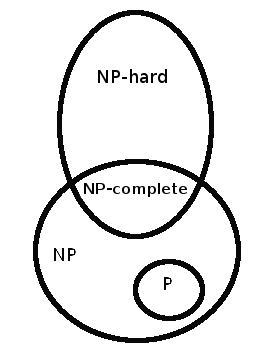
\includegraphics[width=5cm, height=8cm]{pnp2}
        \caption{Tipos de complejidades computacionales}
    \end{figure}
    
    
    \paragraph{}
    De los tipos de complejidades computacionales descritos, la \textbf{complejidad máxima para cualquier problema de planificación es la máxima complejidad posible, es decir, es NP-hard}.\cite{backstrom1995complexity}
    
    
            \subsubsection{Planificadores utilizados}
    
                \setcounter{subsubsubsection}{0}
                \subsubsubsection{Metric-FF}
    \paragraph{}
    \textit{Metric-FF}\cite{mff} es un \textbf{planificador independiente de dominio} que \textbf{permite operar} con sentencias de \textit{PDDL 2.1} y \textbf{con sentencias numéricas con dígitos}. Este planificador es una extensión del planificador \textit{FF} para incluir construcciones numéricas\cite{ff1} que resuelvan tareas lineales (es decir, que el valor de las variables numéricas pueda ser modificado mediante los operadores de suma y resta, excluyendo otras operaciones como la multiplicación o la división). Está implementado en \textit{C}, ambos desarrollados por Joerg Hoffmann bajo la licencia de \textit{GNU General Public License}. \textit{Metric-FF} fue uno de los planificadores presentados en la tercera edición de la \textit{IPC} obteniendo el mejor desempeño de todos los planificadores en el track numérico\cite{mffIPC3}. Existen a su vez otras versiones de \textit{FF}, como pueden ser \textit{Conformant-FF}, \textit{Contingent-FF}\cite{conformant} o \textit{FF-X}.
    
    \paragraph{}
    Para poder buscar una solución,el planificador necesita un árbol de estados, un valor heurístico para cada estado del árbol de estados y un algoritmo de búsqueda que permita buscar soluciones en dicho árbol. Este árbol se configura mediante una relajación de las condiciones del problema inicial y un intento de buscar una solución al problema relajado, por ejemplo mediante la conservación de los estados eliminados por las acciones. Lo que diferencia a esta extensión llamada \textit{Metric-FF} del planificador \textit{FF} original es que también utiliza también técnicas de relajación de las cláusulas para los dominios numéricos con dígitos. Estas técnicas incluyen en los dominios numéricos la relajación de decrementos de las variables numéricas, puesto que en estos dominios estas variables cuando aparecen en la parte de los efectos de los operadores, suelen aparecen en calidad de variación de sus valores (incrementos o decrementos de los mismos) en lugar de por eliminación de las variables en sí. Sin embargo, para que esta relajación del problema sea válida se debe comprobar antes que siempre es preferible tener valores elevados (a estos problemas se les llama \textit{monotónicos}) para poder alcanzar la solución, ya que de no ser así se podría incluso perder la solución al intentar relajar el problema.
    
    \paragraph{}
    \textbf{El proceso de búsqueda de la solución se realiza utilizando el algoritmo de búsqueda en escalada o \textit{Enforced Hill Climbing} (\textit{EHC})}. Este algoritmo es una variación del algoritmo de búsqueda de colina o \textit{Hill Climbing}. Antes de explicar la particularidad del algoritmo utilizado en \textit{Metric-FF} respecto al algoritmo de \textit{Hill climbing}, se va a explicar cómo funciona este último.
    
    \paragraph{}
    El algoritmo de \textit{Hill climbing} es un algoritmo de \textbf{búsqueda local} iterativo que expande el estado inicial hasta encontrar un estado que sea la solución. Es un algoritmo de búsqueda local sin memoria que genera iterativamente los sucesores del último estado expandido. De estos sucesores, el mejor de estos sucesores es el que se expande. En caso de que el sucesor no sea mejor que el estado padre, la búsqueda falla.
    
    \paragraph{}
    La diferencia entre este algoritmo y \textit{Enforced Hill Climbing} reside en que mientras que en \textit{Hill Climbing} \textbf{la mejora iterativa} se hace mediante la selección de uno de los mejores sucesores del estado actual, en \textbf{\textit{Enforced Hill Climbing} se utiliza una búsqueda en anchura} o \textit{breadth first seach} para encontrar el primer sucesor cuya evaluación heurística sea mejor que la del nodo actual. El \textit{problema} que tienen ambos algoritmos es que al ser una búsqueda local, este algoritmo \textbf{falla en caso de que los valores heurísticos de los sucesores se topen con mínimos locales}, lo que se da si todo sucesor tiene peor valor heurístico, por lo que el algoritmo no hallaría ninguna de las rutas por las que se llega a la solución óptima.
    
    \paragraph{}
    Respecto a las fecha primera versión del planificador del que deriva, \textit{FF}, fue publicada en 2001 y la versión de \textit{Metric-FF} utilizada en este trabajo es la versión 2.1 (la última versión) publicada a fecha 04/2017.
                \subsubsubsection{Fast Downward}
    \paragraph{}
    \textit{Fast Downward}\cite{fastDownward} es un planificador que puede solucionar problemas expresados en \textit{PDDL}. Al igual que ocurre con \textit{FF}, \textit{Fast Downward} es un planificador progresivo. La heurística, que utiliza descomposiciones de las tareas, se denomina heurística de grafo casual. Entre sus logros, se encuentra el ser el planificador ganador del track clásico de la cuarta edición de la \textit{IPC}.
    
    \paragraph{}
    Respecto a la versión utilizada, se ha utilizado la versión presentada en la \textit{IPC} de 2011.
    
                \subsubsubsection{LPG}
    \paragraph{}
    El planificador \textit{Local Search Planner} (\textit{LPG})\cite{lpg} es, al igual que los planificadores anteriores, un planificador independiente de dominio y su primera versión salió a la luz en el año 2003. Este planificador utiliza varias heurísticas basadas en una función de evaluación parametizada donde los parámetros son evaluados dinámicamente. Es un \textbf{planificador incremental que produce planes basados en varios criterios de calidad}. El núcleo de este planificador está basado en \textbf{búsquedas estocásticas locales} y en una representación basada en grafos llamada Grafos de Acción Temporales (\textit{TA-graphs}).
    
    \paragraph{}
    Para realizar la búsqueda local, \textit{LPG} utiliza el algoritmo \textit{Walkplan} con el fin de encontrar el grafo de solución. Para ello, primeramente habrá que generar un grafo de acciones (\textit{A-graph}) inicial, siendo un grafo de acción un subgrafo de un grafo de planificación conteniendo los nodos de acciones iniciales y los nodos de acciones finales (que son el último paso antes de alcanzar la solución). Si un nodo de acción del grafo de planificación está en este grafo de acción entonces también los nodos correspondientes a las precondiciones y los efectos positivos de estas acciones deben estar en este nuevo grafo de acciones.
    
    \paragraph{}
    Este \textit{A-graph} inicial podrá ser generado de diversas maneras, como puede ser generando un grafo vacío o inicializado aleatoriamente (este segundo caso explica por qué este planificador es estocástico). Una vez se ha generado este grafo inicial, se pueden añadir o quitar nodos de acción hasta llegar a encontrar una solución.
    
    \paragraph{}
    La versión utilizada en las pruebas es la versión de 2004, \textit{LPG-td}, ya que esta versión introduce la mejora respecto a la versión 1.2 de poder resolver problemas numéricos.
    
    \subsection{Modificadores automáticos de dominios y problemas}
    
    \paragraph{}
    En esta sección se van a explicar en qué consisten algunos de los modificadores automáticos de dominios independientes de dominio. La mayor parte de estos modificadores utilizan exclusivamente una única estrategia genérica para modificar ese dominio sin alternarla con otras posibilidades. Las estrategias más frecuentes suelen ser: la representación de los dominios y problemas en formato numérico con dígitos o con proposiciones o el aglutinamiento de varios operadores en macrooperadores.
    
    \subsubsection{Generadores de macrooperadores}
    
    \paragraph{}
    Los macrooperadores son la unión de varios operadores en un solo operador que tienen por \textbf{objetivo servir como atajo a la resolución de problemas al poder realizar las acciones equivalentes a varios operadores con un solo operador}. Estos macrooperadores \textbf{pueden ser perjudiciales} para la resolución de problemas de planificación ya que \textbf{tienden a incrementar el factor de ramificación} durante la búsqueda de la solución, puesto que por lo general los macrooperadores suelen incrementar el número de operadores aplicable, incrementando a su vez la memoria consumida por el planificador. Por ello la utilización de los macrooperadores no siempre mejora los tiempos de búsqueda de la solución por parte del planificador ni la calidad de la misma (entendida como el número de pasos para llegar a la solución o el valor de la métrica que haya que minimizar o maximizar según sea definido en el problema). Deberán ser los propios algoritmos generadores de estos macrooperadores quienes deban tener en cuenta estos contrapuntos y, en caso de que el generador esté bien programado, no genere macrooperadores en aquellos problemas en los que los inconvenientes no compensen la mejora que aportan dichos cambios y por tanto devuelvan los dominios como se encontraban originalmente. Este problema recibe el nombre de \textbf{"el problema de la utilidad"}.
    
    \paragraph{}
    Respecto a la longitud de estos macrooperadores, trabajos recientes han demostrado que \textbf{es mejor generar pocos macrooperadores y con un tamaño pequeño que generar muchos macrooperadores y con un tamaño grande}. Puesto que las diferentes versiones del dominio utilizado para las pruebas empíricas que aparecen en la sección de ola solución propuesta incluyen varias versiones con macrooperadores de los dos tipos, esta afirmación se pondrá a prueba con los resultados obtenidos para este caso concreto (aun sabiendo que de un caso tan específico no es posible sacar conclusiones más que el servir como un apoyo más de dicha afirmación y no una generalización).
    
    \paragraph{}
    A continuación se incluye la descripción de algunos ejemplos de generadores automáticos de macrooperadores, siendo todos ellos independientes de dominio.
    
    \comment{Incluir definición de generadores de macros online y offline}
    \setcounter{subsubsubsection}{0}
    \subsubsubsection{Planning Task Transformer}
    \paragraph{}
    El generador de macrooperadores \textit{Planning Task Transformer} (\textit{PTT})\cite{chrpa2010generation} es un generador \textit{offline} que se basa en la \textbf{búsqueda de enredos} (\textit{entanglements}) -es decir, la relación de los operadores y los predicados- \textbf{que pueden luego llegar a convertirse en macrooperadores}. A su vez estos macrooperadores son aprendidos a partir de los planes, pues es en estos planes donde se puede observar por ejemplo si dos acciones que actualmente no son adyacentes pueden llegar a serlo mediante permutaciones del órden de ejecución de los operadores. Los macrooperadores se generan según varios criterios, como puede ser el tamaño del macrooperador que se va a generar, el número de veces que se sucede la secuencia de operadores encapsulados o el número de macrooperadores totales generados, aunque PTT no tiene un límite fijo de macrooperadores que pueden llegar a generarse. Por otro lado, la eliminación de todo los operadores encapsulados por estos macrooperadores generado con \textit{PTT} puede implicar la pérdida de la completitud. Sin embargo, las pruebas realizadas por los desarrolladores de este generador demuestran que por lo menos en los dominios presentados a las competiciones de la \textit{IPC}, esta eliminación haría perder la solvabilidad muy raramente.
    
    \paragraph{}
    Respecto a los enredos en los que se basan estos macroopedores, en \textit{PTT} se distinguen los \textbf{enredos externos} y los \textbf{enredos internos}.
    
    \paragraph{}
    Los enredos externos capturan relaciones causales entre los predicados iniciales o los predicados meta y se utilizan para podar instancias poco prometedoras de los operadores. Estos enredos se deducen a partir de los planes de los problemas y uno de los parámetros que se introduce como entrada para determinar cuál de los enredos puede pasar a convertirse en un macrooperador es el porcentaje de veces que dicho enredo no se respeta en alguno de los planes, y se denomina \textit{flaw ratio}. \textbf{Encontrar estos enredos tiene una complejidad de \textit{PSPACE-complete}, por ello estos enredos se deducen mediante algoritmos de aproximación} que tienen menor complejidad, teniendo como contrapunto que la transformación de estos enredos en macrooperadores que sustituyan a los operadores iniciales generalmente no conserva la completitud. Sin embargo, los enredos no siempre se traducen en la generación de macrooperadores. El resultado final que se obtiene es que \textit{PTT} conserva la completitud debido a que sólo se añaden un subconjunto de los macrooperadores derivados de los enredos externos que permiten que ésta se mantenga.
    
    \paragraph{}
    Los enredos internos se producen entre dos operadores en el que uno de ellos produce un predicado que es requerido (o consumido) por un segundo operador. Este tipo de enredos también se denominan enredos por sucesión o por predecesión (en función de si se está refiriendo al sucesor del productor o al predecesor del consumidor).
    
    
    \subsubsubsection{Marvin}
    \paragraph{}
    \textit{Marvin} es un planificador automático desarrollado a partir de \textit{FF}, lo que queda patente en cosas como que comparten entre sí el uso de EHC como algoritmo de búsqueda o que ambos realicen el proceso de búsqueda hacia adelante. La diferencia más importante es que \textbf{\textit{Marvin} incluye una generación de macrooperadores} para la posterior búsqueda de la solución, mientras que \textit{FF} realiza esta búsqueda sin realizar este paso previo. En las siguientes líneas se va a intentar explicar cómo funciona dicho módulo del planificador.
    
    \paragraph{}
    Este planificador \textbf{utiliza los macrooperadores como medio para intentar escapar de los \textit{plateaus}}, ya que estos son los responsables de que los algoritmos de búsqueda local se queden estancados y pierdan la mayor parte del tiempo de búsqueda del algoritmo. Como \textit{Marvin} utiliza el algoritmo de búsqueda local \textit{EHC}, evitar caer en estos \textit{plateaus} es una tarea fundamental para reducir los tiempos de búsqueda.
    
    \paragraph{}
    \textbf{Los macrooperadores son seleccionados en función de las veces que se repita el mismo \textit{plateau} con diferentes problemas}. También influye en el proceso de selección de macrooperadores el tamaño de dicho \textit{plateau}, habiendo una correspondencia directa entre la probabilidad de que un macrooperador sea seleccionado y el tamaño del \textit{plateau} en cuestión. Esto quiere decir que al contrario que en el caso de \textit{PTT}, con \textit{Marvin} se potencian los macrooperadores de mayor tamaño.
    
    \paragraph{}
    Por último, es importante comprobar que los macrooperadores utilizados tienen el mínimo impacto en la longitud del plan: no debe existir una secuencia de operadores iniciales que conlleve al resultado en menos pasos que la aplicación de dicho macrooperador.
    
    \subsubsection{Partición de operadores}
    \paragraph{}
    Como se ha comentado el la sección anterior, \textbf{el beneficio de la inclusión de macrooperadores en la planificación automática está en disputa con otras pérdidas que influyen en la calidad y en el tiempo de búsqueda}. A esta disputa entre pérdidas y ganancias se le denomina \textbf{\textit{el problema de la utilidad}}.
    
    \paragraph{}
    La partición de operadores parte de esta misma base y tiene el enfoque complementario: algunos operadores al ser fragmentados permitirán obtener beneficios en cuanto a la calidad y al tiempo de búsqueda del planificador debidos a la disminución del tamaño de la interfaz de los operadores. En contraste con las técnica de generación de macrooperadores, la segmentación de operadores ha sido mucho menos estudiada entre la comunidad científica.
    
    \paragraph{}
    La modificación de segmentar las acciones en otras más pequeñas es un tipo de modificación del dominio que es muy frecuente en modificaciones realizadas a mano sobre dominios. La principal ventaja de esta técnica es la redución de los operadores básicos o \textit{ground operators}. Por ejemplo, dada una acción $a[X]$ con un tamaño de interfaz $|X|$, su segmentación creará los operadores $a_1[X_1],...,a_k[X_k]$. Si por ejemplo cada $x \in X$ puede ser instanciada con 100 objetos, $|X|=3$ y $|X_i|=1$ (el tamaño de la interfaz para cada operador tras la segmentación), en el primer caso el número de posibles instancias es $100^3=1.000.000$ mientras que en el caso segmentado sería de $100*3=300$.
    
    \paragraph{}
    Para que una separación de operadores sea válida, se deben cumplir las siguientes condiciones:
    \begin{itemize}
        \item Los operadores $a_i[X],...,a_k[X]$ deben de ejecutarse en bloque (sin que se ejecuten otras acciones de por medio) y respetando el órden en que lo hacían los operadores iniciales.
        \item Los operadores $a_i[X],...,a_k[X]$ deben estar configurados de tal manera que al ser ejecutados se asegure que el o los predicados utilizados por estas acciones se mantenga a lo largo de la ejecución. Esto quiere decir que por ejemplo no sea posible que cambie uno de los predicados y por tanto las acciones segmentadas den un resultado distinto de la ejecución de la acción original.
    \end{itemize}
    
    \paragraph{}
    Un ejemplo de software de partición de operadores es     \textit{Automatic Action Schema Splitting}\cite{areces2014optimizing}.
    
    \subsubsection{Reprentación numérica con dígitos}
    \paragraph{}
    Este tipo de modificadores se basa en detectar conjuntos de predicados declarados en el problema que pueden ser agrupados y usados indistintamente, por lo que se puede 
    
    
    \subselub identificasect cada uno de estos predicados por la declaración de un único predicado numérico que sustituya a estos predicados.
    
    \paragraph{}
    La funciones numéricas con dígitos fueron introducidas en \textit{PDDL} en su versión 2.1, sin embargo, no todos los planificadores desarrollados en los últimos años aceptan este tipo de representación. De los planificadore que se han utilizado para las pruebas, \textit{Metric-FF} y \textit{LPG-td} aceptan este tipo de representación, a diferencia de \textit{FastDownward} que no es capaz de interpretar funciones numéricas.
    
    \paragraph{}
    Entre las pruebas realizadas en este estudio, se encuentran los dominios y problemas obtenidos tras la ejecución de un modificador automático de este tipo desarrollado en la Universidad Carlos III de Madrid\cite{fuentetaja2016compiling}.
    
    \subsubsection{Representación numérica con proposiciones}
    \paragraph{}
    Esta representación se basa en el mismo principio que la representación numérica con dígitos: en determinados problemas, existen predicados que pueden perder su identidad y ser cuantificados en función del número de ellos que se hayan definido. La principal diferencia entre ambos tipos de cambio de representaciones es que en este caso la representación numérica no es con dígitos sino con proposiciones.
    
    \paragraph{}
    Entre las pruebas realizadas en este estudio, se encuentra un tipo de modificador de la representación de problemas que realiza este tipo de transformaciones: \textit{Baggy}\cite{riddleimproving}.
    
    \paragraph{}
    Este modificador transforma la representación de dominios y problemas en \textit{PDDL} en una segunda que reduce el tamaño del espacio de estados, eliminando a su vez la explosión combinatoria. Los pasos que se deben seguir para resolver un problema utilizando \textit{Baggy} son los siguientes:
    \begin{enumerate}
        \item Determinar qué elementos pueden ser agrupados y \textbf{reformulación} de la representación de \textit{PDDL}.
        \item \textbf{Resolución} de la planificación con la nueva representación.
        \item \textbf{Transformación} del problema del espacio de estados nuevos al espacio de estados original.
    \end{enumerate}
    
    \paragraph{}
    Una ventaja de este tipo de modificaciones respecto a las modificaciones que incorporan funciones numéricas con dígitos es que en este caso la nueva representación generada puede ser resuelto por cualquier planificador que pueda interpretar problemas en \textit{PDDL}.
    
            \subsubsection{Dominios utilizados}
    
    \paragraph{}
    Todos los dominios y problemas utilizados están escritos en \textit{PDDL} y consisten en modificaciones del \textbf{dominio original de \href{https://helios.hud.ac.uk/scommv/IPC-14/repository/benchmarksV1.1.zip}{Child-Snack} utilizado en la \textit{IPC} de 2014\cite{ipc2014}}. Los dominios utilizados para las pruebas de la inmensa mayoría de los trabajos de planificación automática citados en este documento provienen también de esta competición, en la cual hay varios dominios que se repiten o se actualizan entre las distintas ediciones, por lo cual se cree que la utilización exclusiva de dominios pertenecientes a la \textit{IPC} puede permitir que otros investigadores puedan problematizar y comparar los resultados obtenidos en este trabajo con otras investigaciones con mayor facilidad, ya que por lo que se ha dicho se comparte el marco de problemas utilizado con muchas de las investigaciones recientes en este área.
    
    %\medskip
    \pagebreak
    
    \section{Desarrollo del trabajo}
    
    \paragraph{}
    Para el desarrollo de este proyecto \textbf{se ha utilizado} software de terceros que en todas las etapas del mismo ha sido \textbf{exclusivamente software libre y gratuito} motivo por el cual no va a ser señalada esta característica para cada una de las herramientas utilizadas que será citada a continuación. En esta sección se puede encontrar la descripción de todos los dominios utilizados así como de las herramientas para su desarrollo y posterior testeo.
    
    \subsection{Herramientas de desarrollo utilizadas}
    \paragraph{}
    En esta sección se detallan todas las herramientas tecnológicas utilizadas para el desarrollo de este proyecto. Como el hardware utilizado afecta exclusivamente al desempeño de las pruebas funcionales, estas características se incluirán en la sección de resultados obtenidos.
    
    \subsubsection{Sistema operativo}
    
    \paragraph{}
    El sistema operativo utilizado en cada una de las etapas del proceso ha sido \textbf{Debian GNU-Linux} versión 8.7. Este sistema operativo ha sido elegido para el proyecto ya que por una parte algunos de los programas de terceros desarrolladores están pensados para ser utilizados en sistemas operativos GNU/Linux y por otra se tenía cierta familiaridad previa con el mismo. Este sistema operativo puede descargarse en la siguiente página web: www.debian.org [última vez visitada: 18/05/2017].
    
    \subsection{Edición de código}
    \paragraph{}
    El código ha sido editado y desarrollado mediante el editor de texto plano \textbf{Gedit}, que es un editor el cual viene incluído en el paquete de instalación básico de muchas distribuciones de GNU-Linux. Puede descargarse en la siguiente página web: \\ www.wiki.gnome.org/Apps/Gedit [última vez visitada: 18/05/2017]. Este editor ha sido utilizado por su sencillez. Sin embargo, para proyectos más complejos puede ser mejor utilizar otros editores como Vim\footnote{www.vim.org} o Emacs\footnote{https://www.gnu.org/software/emacs/}, ambos de software libre y gratuito.
    
    \subsection{Control de versiones}
    \paragraph{}
    Para el control de versiones de código se ha utilizado un repositorio de \textbf{Git} alojado en GitHub con un único repositorio para alojar todo el código utilizado así como otro repositorio para las distintas versiones de la memoria.
    
    \paragraph{}
    De esta manera, en caso de pérdida o avería del dispositivo con el que se ha desarrollado este proyecto, existía una copia de seguridad de todo el trabajo realizado en GitHub.
    
    \paragraph{}
    Al haberse escrito esta memoria en un formato que antes de ser transformado a formato \textit{PDF} es texto plano (en contraposición con el formato de texto enriquecido de editores como LibreOffice Writer), en lugar de usar un repositorio de documentos como Alfresco\footnote{www.alfresco.com}, se ha podido crear otro repositorio de Git que detectase los cambios entre las distintas versiones de la memoria.
    
    \subsection{Edición de la memoria}
    \paragraph{}
    La memoria ha sido desarrollada en \textbf{\LaTeX{} (latex)} y en este caso por comodidad ha sido escrita en el editor en línea de Sharelatex. Esto es debido únicamente a que a diferencia de lo que ocurre con el editor Gedit estándar (es decir, sin añadir ningún complemento), en este editor en línea es posible comprobar los errores de sintaxis antes de haber compilado el archivo así como el hecho de que la propia interfaz permite visualizar en una única ventana el documento PDF que se va a generar y ver la correspondencia entre la salida en dicho PDF con la línea exacta del archivo de latex que la genera.
    
    \paragraph{}
    Una vez modificados los documentos en Sharelatex, estos eran pasados a Git de forma manual: el proyecto de Sharelatex era descargado y después subido a Git como \textit{commit} con los cambios que detectase.
    
    \subsection{Scripts para la traducción de problemas manuales}
    \paragraph{}
    La mayoría de las versiones de los dominios y problemas realizados a mano han sido realizados mediante scripts que tuviesen como parámetro de entrada el problema original y como archivo de salida el problema en la versión modificada a mano correspondiente. Estos scripts se han realizado en el lenguaje de programación \textbf{Python}.
    
    \subsection{Scripts para la generación de problemas automáticos}
    \paragraph{}
    Los scripts de terceros utilizados para la transformación automática de dominios generan un dominio por cada ejecución. Con el fin de automatizar la transformación de todos los problemas, se han creado varios un script en \textbf{Bash} para cada uno de los modificadores para así poder obtener todos los problemas modificados a partir de aquellos que se encuentren en un directorio especificado sin tener que ejecutar a mano cada uno de estos scripts de transformación por cada uno de los problemas a transformar.
    
    \subsection{Scripts para la automatización de pruebas}
    Se ha realizado un script en \textbf{Bash} que permite obtener los tiempos de ejecución y la calidad de la solución de la planificación automática de la versión del dominio y los problemas que se introduzcan como parámetros para los planificadores \textit{Metric-FF} y \textit{LPG-td}. En la sección de evaluación de resultados se concreta exactamente en qué consisten estas pruebas.
    
    \subsection{Descripción de los dominios}
    
    \paragraph{}
    
    En esta sección se van a describir todos los dominios utilizados en el proyecto
    como entrada de los distintos planificadores utilizados en la fase de obtención
    de tiempos y de calidad de las soluciones para su ulterior análisis. 
    
    \paragraph{}
    Todas las versiones de dominios utilizados provienen de la edición de 2014 de la \textit{IPC}. Todos los dominios analizado son modificaciones del dominio de Childsnack de esta edición. Este tipo de modificaciones, sin embargo, no son exclusivas de un dominio concreto; la correlación entre la modificación de las representaciones y la calidad de las soluciones obtenidas ya ha sido estudiada por otros investigadores\cite{riddle2011does}\cite{riddle2015bagged}.
    
    \paragraph{}
    Las modificaciones realizadas al dominio de \textit{Childsnack} han sido realizadas tanto a mano como mediante software de terceros independiente de dominio.
    
    \paragraph{}
    En el caso de que uno de los dominios derive de otro, únicamente se va a
    explicar en el dominio derivado los motivos y los cambios respecto al dominio
    original. Por último, en todos ellos se explicará si los nuevos dominios son
    completos y si se pierde la optimalidad respecto al dominio original.
    
    \paragraph{}
    El resúmen de los cambios realizados en cada versión se puede encontrar a continuación:
    \begin{itemize}
        \item \textbf{Versión original}: versión sin modificar de \textit{Childsnack}.
        \item \textbf{Versión 01}: utiliza macrooperadores. Junta los operadores \cool{move\_tray} con \cool{serve\_sandwich} y con  \cool{serve\_sandwich\_no\_gluten}, elimina el operador \\ \cool{move\_tray} e incluye el operador \cool{move\_tray\_kitchen} para que las bandejas portátiles no puedan moverse entre las mesas.
        \item \textbf{Versión 02}: cambia el operador \cool{make\_sandwich} para que no acepte como entrada componente y pan sin gluten para que así no lo etiquete como que tuviesen gluten cuando en realidad no lo tienen.
        \item \textbf{Versión 03}: utiliza macrooperadores. Permanecen únicamente los siguientes operadores:\\ \cool{make\_sandwich\_move\_tray\_serve\_sandwich\_no\_gluten\_move\_tray\_kitchen}, \\ \cool{make\_sandwich\_move\_tray\_serve\_sandwich\_gluten\_move\_tray\_kitchen} \\ y \cool{move\_tray\_kitchen}.
        \item \textbf{Versión 05}: es la versión numérica manual con proposiciones.
        \item \textbf{Versión 08}: es la versión numérica manual con dígitos.
        \item  \textbf{Versión 09}: aglutina varios predicados en uno. Se elimina el predicado \\ \cool{(waiting ?c ?p)} para pasar a definir la localización del niño con \\ \cool{(not\_allergic\_gluten ?c ?p)} y \cool{(allergic\_gluten ?c ?p)}.
        \item \textbf{Versión 11}: cambia predicados negativos por la negación de estos predicados en positivo. Cambia los predicados \cool{(not\_allergic\_gluten ?c)} y \cool{(served ?c)} por \cool{(not (allergic\_gluten ?c)} y \cool{(not (waiting ?c))} respectivamente.
        \item \textbf{Versión 12}: versión en la que se segmenta la ejecución en distintas etapas, sin permitir avanzar hasta que se hayan completado las etapas anteriores.
        \item \textbf{Versión PTT}: es la misma que la versión original, porque este software ha sido incapaz de encontrar mejoras a la representación.
        \item \textbf{Versión numérica con proposiciones}: generada automáticamente por \textit{Baggy}.
        \item \textbf{Versión numérica con dígitos}: generada automáticamente. El dominio varía respecto a la versión 08 en que en esta versión se incluyen dos operadores para el operador \cool{serve\_sandwich} de la versión 08. La representación de los problemas es la misma en ambas versiones.
    \end{itemize}
    
    \subsection{Versiones del dominio Childsnack}
    
    \paragraph{}
    A continuación, se encuentra la descripción de todas las versiones del problema de \textit{Childsnack} que han sido utilizadas como entrada de los distintos planificadores para la obtención de resultados que se encuentra en la sección posterior a esta.
    
    \subsubsection{Versión original}
    
    \paragraph{}
    El dominio original recibe el nombre de \textit{Childsnack} y fue presentado por
    primera vez en la edición del año 2014 de la \textit{IPC} (International
    Planning Competition). En este dominio se pretende organizar la creación y
    distribución de sándwiches a partir de unos componentes con y sin gluten para un
    grupo de niños donde parte de ellos puede que sean alérgicos al gluten, por lo
    que en este caso los dos componentes de los sándwiches deberán necesariamente no
    tener gluten. Por otro lado, en el caso de los niños que no son alérgicos al
    gluten será indiferente si alguno o todos los componentes del sándwich contienen
    o no gluten.
    
    \paragraph{}
    Los sándwiches se definen con el predicado \\ \cool{(at\_kitchen\_sandwich ?s -
    sandwich)} y constan de dos componentes: el pan y el contenido, que son
    definidos mediante los predicados \cool{(at\_kitchen\_bread ?b - bread-portion)}
    y \cool{(at\_kitchen\_content ?c - content-portion)}. Todos los sándwiches se hacen
    en la cocina (que se define a su vez mediante la constante \cool{kitchen}) y
    únicamente se gasta un trozo de pan y de componente por cada sándwich. En la
    definición original del dominio, únicamente se puede definir la cocina como
    localización de los componentes del sándwich, a diferencia de lo que ocurre con
    las bandejas portátiles, los sándwiches y los niños. Una vez se ha creado el
    sándwich, los componentes utilizados son eliminados de la lista de hechos (no
    son reutilizables).
    
    \paragraph{}
    Como ya se ha comentado, los componentes de los sándwiches así como el sándwich
    final podrá tener o no gluten. En caso de que alguno de estos elementos tenga
    gluten, no será necesario añadir ningún predicado adicional. Por contra, para
    señalar que uno de estos elementos no contiene gluten se utilizará el predicado
    correspondiente de los siguientes: \cool{(no\_gluten\_bread ?b - bread-portion)}, \cool{(no\_gluten\_content ?c - content-portion)}, \cool{(no\_gluten\_sandwich
    ?s - sandwich)}.
    
    \paragraph{}
    Los sándwiches que se crean en la cocina pueden después ser cargados y
    transportados utilizando bandejas portátiles. Estas bandejas portátiles no tienen
    ninguna restricción en cuanto a cantidad de sándwiches que pueden transportar y
    permiten que los sándwiches puedan ser transportados libremente entre la cocina
    y las distintas localizaciones de los niños, permitiendo a su vez que tanto el
    origen como el destino de la bandeja sean las distintas posiciones de los niños. Las
    bandejas se declaran mediante el predicado \cool{(at ?t - tray ?p - place)}, que
    indica la localización de cada una de ellas.
    
    \paragraph{}
    En caso de que coincida la localización de la bandeja con la cocina, los
    sándwiches que queden creados en la cocina pueden ser cargados en la bandeja, para
    ello se declara el predicado \cool{(ontray ?s - sandwich ?t - tray)}. A su
    vez, en caso de coincidir la localización de la bandeja con la de alguno de los
    niños que aún no haya sido servido y la bandeja esté cargada con algún sándwich
    que se adapte a sus necesidades en cuanto al gluten se refiere, este sándwich
    puede ser eliminado de la bandeja y servido al niño.
    
    \paragraph{}
    Los niños que no han sido servidos y que se espera que tras la resolución del
    problema sean servidos son declarados mediante el predicado
    \cool{(waiting ?c - child ?p - place)} cuando están esperando y con el
    predicado \cool{(served ?c - child)} cuando ya han sido servidos.
    
    \paragraph{}
    La dificultad principal de este dominio se basa en la limitación de componentes
    sin gluten que son necesarios para la creación de sándwiches para los niños
    alérgicos al gluten, ya que en el caso de los no alérgicos cualquier sándwich
    servido resolvería el problema. Esto podría implicar por ejemplo que se
    utilizase erróneamente un componente sin gluten con otro componente con gluten
    que podría ser necesario para crear otro sándwich sin gluten. Sin embargo, en
    otra situación podría ocurrir que dicha combinación fuera correcta ya que no
    quedase otra opción para servir al niño que queda que no es alérgico al gluten.
    A su vez, no se le puede servir a un niño no alérgico al gluten un sándwich
    etiquetado como sin gluten, por lo que la solución de hacer tantos sándwiches
    sin gluten como permita el dominio y después si hace falta distribuir esos
    sándwiches entre los no alérgicos se descarta al no ser una solución válida para
    cualquier problema de entrada.
    
    \paragraph{}
    Al contrario que ocurre con los componentes, para cada niño es necesario
    especificar tanto si son como si no son alérgicos al gluten mediante los predicados \cool{(allergic\_gluten ?c - child)} y \cool{(not\_allergic\_gluten ?c - child)}.
    
    \paragraph{}
    A este problema hay que sumarle que ni el número de niños definidos en el
    problema ni el número de sándwiches máximos que se pueden realizar, definidos
    mediante el predicado \cool{(notexist ?s - sandwich)}, tiene por qué coincidir
    con el número y la composición de alérgicos de niños definidos en la meta como
    que tienen que ser servidos, por lo que incluso aunque se incluyese conocimiento
    del dominio en la resolución del problema por parte del planificador, el
    problema seguiría sin ser trivial. De todas maneras, aunque el predicado \cool{(notexist ?s - sandwich)} se puede utilizar para limitar el número máximo de sándwiches que se pueden realizar, su verdadera función es que exista una correlación de a uno en los sándwiches creados. 
    
    
    \paragraph{}
    Tras haber explicado la idea general del dominio así como sus dificultades a la
    hora de resolver los problemas, se va a explicar la entrada y salida de cada una
    de las acciones del dominio así como la estructura general que deben tener los
    problemas de entrada.
    
    \paragraph{}
    Las acciones del dominio original son:
    \begin{itemize}
        \item \textbf{make\_sandwich\_no\_gluten (porción de pan sin gluten, porción de contenido sin gluten)}
            \begin{itemize}
                \item \textbf{Precondiciones}: que exista al menos un contenido y un trozo de
                pan donde ambos sean sin gluten y haya al menos un hecho de no
                existencia de sandwich. 
                \item \textbf{Efectos}: eliminación de los dos componentes utilizados y del hecho
                de no existencia de sándwich y creación de un sandwich sin gluten.
            \end{itemize}
        \item \textbf{make\_sandwich (porción de pan, porción de contenido)}
            \begin{itemize}
                \item \textbf{Precondiciones}: que exista al menos un contenido y un trozo de
                pan con o sin gluten y haya al menos un hecho de no existencia de
                sándwich.
                \item \textbf{Efectos}: eliminación de los componentes utilizados y del hecho de no
                existencia de sándwich y creación de un sandwich etiquetado como
                con gluten (aún en el caso de que ambos elementos utilizados no
                tengan gluten).
            \end{itemize}
        \item \textbf{put\_on\_tray (sándwich, bandeja portátil)}
            \begin{itemize}
                \item \textbf{Precondiciones}: que exista al menos un sándwich en la cocina y
                que al menos una de las bandejas portátiles esté en la cocina.
                \item \textbf{Efectos}: carga uno de los sándwiches en una de las bandejas
                portátiles que esté en la cocina.
            \end{itemize}
        \item \textbf{serve\_sandwich\_no\_gluten (sándwich sin gluten, bandeja portátil, niño, posición)}
            \begin{itemize}
                \item \textbf{Precondiciones}: que al menos una de las bandejas portátiles esté
                en la misma posición que uno de los niños, que la bandeja que cumpla
                la precondición anterior tenga al menos un sándwich sin gluten, que
                un niño no alérgico al gluten esté en la misma localización que la
                bandeja que cumple las precondiciones anteriores y que este mismo niño esté esperando un sándwich.
                \item \textbf{Efectos}: el niño pasa a estar servido y se elimina el sándwich utilizado en la operación.
            \end{itemize}
        \item \textbf{serve\_sandwich (sándwich, bandeja portátil, niño, posición)}
            \begin{itemize}
                \item \textbf{Precondiciones}: que al menos una de las bandejas portátiles esté
                en la misma posición que uno de los niños, que la bandeja que cumpla la
                precondición anterior tenga al menos un sándwich con o sin gluten,
                que un niño no alérgico al gluten esté en la misma localización que la
                bandeja que cumple las precondiciones anteriores y que este mismo
                niño esté esperando un sándwich.
                \item \textbf{Efectos}: el niño pasa a estar servido y se elimina el sándwich
                utilizado en la operación.
            \end{itemize}
        \item \textbf{move\_tray (bandeja portátil, posición inicial, posición final)}
            \begin{itemize}
                \item \textbf{Precondiciones}: que la bandeja esté en la localización inicial.
                \item \textbf{Efectos}: mueve la bandeja de su localización inicial a una nueva
                localización.
            \end{itemize}
        
    \end{itemize}
    
    \paragraph{}
    En el problema se podrán definir los siguientes elementos:
    \begin{itemize}
        \item Bandejas portátiles, con la localización inicial de cada uno de ellos.
        \item Panes que se encuentran en la cocina.
        \item Contenidos (de los sándwiches) que se encuentran en la cocina.
        \item Especificación de los trozos de pan que no llevan gluten.
        \item Especificación de los contenidos que no llevan gluten.
        \item Especificación de los niños alérgicos al gluten.
        \item Especificación de los niños que no son alérgicos al gluten.
        \item Especificación de los niños que están esperando que les sirvan un sándwich y su localización.
        \item Especificación de los niños que tienen que ser servidos para resolver el problema.
    \end{itemize}
    
    
    \subsubsection{Versiones modificadas a mano}
    
    \paragraph{}
    En esta sección se describen los dominios que han sido generados a mano, en contraposición con los dominios generados mediante software de terceros que serán explicados en la sección que se encuentra a continuación de esta.
    
     \setcounter{subsubsubsection}{0}
    \subsubsubsection{Versión 01}
    
    \paragraph{}
    Mientras que la definición de los problemas en este dominio no varía
    respecto a la definición original, en la definición del dominio se han añadido 
    macrooperadores de las acciones \cool{move\_tray} con las acciones
    \cool{serve\_sandwich} y \\
    \cool{serve\_sandwich\_no\_gluten}, quedando por tanto los macrooperadores \\
    \cool{move\_tray\_serve\_sandwich} y \cool{move\_tray\_serve\_sandwich\_no\_gluten}. La inclusión de macrooperadores también ha implicado la inclusión de la función numérica \cool{total\_cost}, inicializada a cero en cada uno de los problemas de entrada. Esta función es utilizada tanto en esta versión como en la versión 03 y en ambas tiene exactamente la misma razón de ser: aumenta su valor al ejecutar los operadores en tantas unidades como operadores del problema inicial esté sustituyendo, teniendo entre las métricas de sus problemas la reducción de su coste. Esto implica que los dos operadores utilizados en este dominio incrementan dicho valor en dos unidades mientras que  el resto de operadores al ser los operadores iniciales incrementan su valor en una unidad. El motivo de la inclusión de esta función es que por un lado de esta manera al obtener el coste total de la solución no se obtienen costes artificialmente bajos (como sucedería si no coincidiese e coste de un macrooperador que el de los operadores contenidos) y por otro, al introducir la métrica de su reducción, los planificadores podrán tener esto en cuenta durante su planificación con el fin de obtener soluciones de menor coste.
    
    \paragraph{}
    Respecto a los macrooperadores mencionados en el párrafo anterior, estos tienen como fin unir la acción de mover la bandeja con la acción de
    servir el sándwich ya que viendo la resolución de problemas se puede comprobar
    con facilidad que la solución óptima tras mover la bandeja a una mesa es servir
    al menos un sándwich, ya que el objetivo de dicho desplazamiento es
    exclusivamente servir dicho sándwich que además es justo la siguiente acción a realizar,
    por lo que intuitivamente tiene sentido unir ambas acciones, así como añadir
    una acción para mover la bandeja a la cocina para volver a cargarlo.
    
    \paragraph{}
    Los nuevos macrooperadores incrementan el número de parámetros de las
    precondiciones del operador, pasando de dos a cuatro. A su vez, implica
    aumentar el factor de ramificación, ya que se ha aumentado en dos el número de
    operadores disponibles.
    
    \paragraph{}
    En lo que concierne tanto a la completitud y a la optimalidad, siempre que se
    añadan macro-operadores sin eliminar los operadores originales ambas
    condiciones se conservarán, puesto que en el peor de los casos en los que no se pueda
    obtener la solución óptima o completa utilizando los macro-operadores, siempre
    estará la opción de utilizar los operadores originales. En este caso, si se eliminasen
    los operadores originales \cool{move\_tray}, \cool{serve\_sandwich} y \cool{serve\_sandwich\_no\_gluten}
    contenido en los nuevos macro-operadores y se añadiese a su vez el operador
    \cool{move\_tray\_kitchen}, el dominio sería completo puesto que todas las soluciones
    del dominio original están contenidas en el nuevo dominio. Sin embargo, este
    dominio no sería óptimo puesto que al perder el operador \cool{move\_tray}, en todos
    los problemas en los que los niños estuvieran en varias localizaciones, sería
    necesario que una vez servido a el/los niño/s de la primera localización, se volviese
    necesariamente a la cocina para poder volver a mover la bandeja y servir a el/los
    siguiente/s niño/s, perdiendo por tanto la solución óptima al tener que realizar
    el movimiento innecesario respecto al dominio original de tener que volver a la
    cocina para poder servir el/los siguiente/s sándwich/es. Para que quede este
    punto más claro, se va a mostrar un ejemplo de un problema muy sencillo en
    el que se puede ver claramente cómo se produce esta pérdida de la solución
    óptima.
    
    \paragraph{}
    Definición del problema de ejemplo:
    \begin{itemize}
        \item Pan \cool{bread1} con gluten
        \item Pan \cool{bread2} sin gluten
        \item Contenido \cool{content1} con gluten
        \item Contenido \cool{content2} sin gluten
        \item Niño \cool{child1} alérgico al gluten
        \item Niño \cool{child2} no alérgico al gluten
        \item Niño \cool{child1} en table1
        \item Niño \cool{child2} en table1
        \item bandeja \cool{tray1} en kitchen
    \end{itemize}
    
    \textbf{Solución óptima con el dominio original}: \\
    
    \noindent \cool{0: (MAKE\_SANDWICH\_NO\_GLUTEN SANDW1 BREAD1 CONTENT1) \\
    1: (MAKE\_SANDWICH SANDW2 BREAD2 CONTENT2) \\
    2: (MAKE\_SANDWICH SANDW3 BREAD3 CONTENT3) \\
    3: (PUT\_ON\_TRAY SANDW1 TRAY1) \\
    4: (PUT\_ON\_TRAY SANDW2 TRAY1) \\
    5: (PUT\_ON\_TRAY SANDW3 TRAY1) \\
    6: (MOVE\_TRAY TRAY1 KITCHEN TABLE1) \\
    7: (SERVE\_SANDWICH\_NO\_GLUTEN SANDW1 CHILD1 TRAY1 TABLE1) \\
    8: (SERVE\_SANDWICH SANDW2 CHILD2 TRAY1 TABLE1) \\
    9: (SERVE\_SANDWICH SANDW3 CHILD3 TRAY1 TABLE1) \\}
    
    \paragraph{}
    \textbf{Solución con la versión 01 \underline{sin} los operadores iniciales}: \\
    \noindent \cool{0: (MAKE\_SANDWICH SANDW3 BREAD3 CONTENT3) \\
    1: (MAKE\_SANDWICH SANDW2 BREAD2 CONTENT2) \\
    2: (MAKE\_SANDWICH SANDW1 BREAD1 CONTENT1) \\
    3: (PUT\_ON\_TRAY SANDW1 TRAY1) \\
    4: (PUT\_ON\_TRAY SANDW2 TRAY1) \\
    5: (PUT\_ON\_TRAY SANDW3 TRAY1) \\
    6: (MOVE\_TRAY\_SERVE\_SANDWICH\_NO\_GLUTEN TRAY1 KITCHEN TABLE1 SANDW1 CHILD1) \\
    7: (MOVE\_TRAY\_KITCHEN TRAY1 TABLE1) \\
    8: (MOVE\_TRAY\_SERVE\_SANDWICH TRAY1 KITCHEN TABLE1 SANDW2 CHILD2) \\
    9: (MOVE\_TRAY\_KITCHEN TRAY1 TABLE1) \\
    10: (MOVE\_TRAY\_SERVE\_SANDWICH TRAY1 KITCHEN TABLE1 SANDW3 CHILD3)} \\
    
    \paragraph{}
    \textbf{Solución con la versión 01 \underline{con} los operadores iniciales}: \\
    \noindent \cool{0: (MAKE\_SANDWICH\_NO\_GLUTEN SANDW1 BREAD1 CONTENT1) \\
    1: (MAKE\_SANDWICH SANDW2 BREAD2 CONTENT2) \\
    2: (MAKE\_SANDWICH SANDW3 BREAD3 CONTENT3) \\
    3: (PUT\_ON\_TRAY SANDW1 TRAY1) \\
    4: (PUT\_ON\_TRAY SANDW2 TRAY1) \\
    5: (PUT\_ON\_TRAY SANDW3 TRAY1) \\
    6: (MOVE\_TRAY\_SERVE\_SANDWICH\_NO\_GLUTEN TRAY1 KITCHEN TABLE1 SANDW1 CHILD1) \\
    7: (SERVE\_SANDWICH SANDW2 CHILD2 TRAY1 TABLE1) \\
    8: (SERVE\_SANDWICH SANDW3 CHILD3 TRAY1 TABLE1)} \\
    
    \paragraph{}
    Como se puede ver, estando la bandeja ya en la misma posición que \cool{child2} y \cool{child3}, sin los operadores iniciales necesita volver a la cocina para poder servirles, por lo que queda demostrado con este ejemplo que los operadores iniciales son necesarios para conservar la optimalidad. Por este motivo, se van a conservar dichos operadores en la versión final de esta versión.
    
    \subsubsubsection{Versión 02}
    
    \paragraph{}
    La defición de los problemas no varía respecto a la definición original, por lo que en las siguientes líneas se va a explicar en qué varía este nuevo dominio respecto a la definición original. Únicamente se han modificado las precondiciones de único operador \cool{make\_sandwich}. En el dominio original, todos los sándwiches creados con este operador no son etiquetados como que no tuvieran gluten aún cuando ambos componentes utilizados no contengan gluten. Este supuesto no tiene ningún sentido, ya que implica que se están etiquetando erróneamente sándwiches que realmente no tienen gluten por haber pasado por este operador en lugar de por el operador \cool{make\_sandwich\_no\_gluten}, lo que implica que el propio operador permite que se generen ramas del árbol de decisión que podrían producirse a través del otro operador mencionado, por lo que están duplicados.
    
    \paragraph{}
    Para entender mejor esta modificación, se va a incluir un problema base con un grafo de búsqueda del camino que conecte el estado inicial con la solución con el dominio original y otro grafo de búsqueda con este nuevo dominio.
    
    \paragraph{}
    El problema en cuestión es el siguiente:
    \begin{itemize}
        \item 1 pan sin gluten
        \item 1 componente sin gluten
        \item 1 bandeja en la cocina
        \item 1 niño alérgico al gluten en table1
    \end{itemize}
    
    \begin{figure}[H]
        \centering
        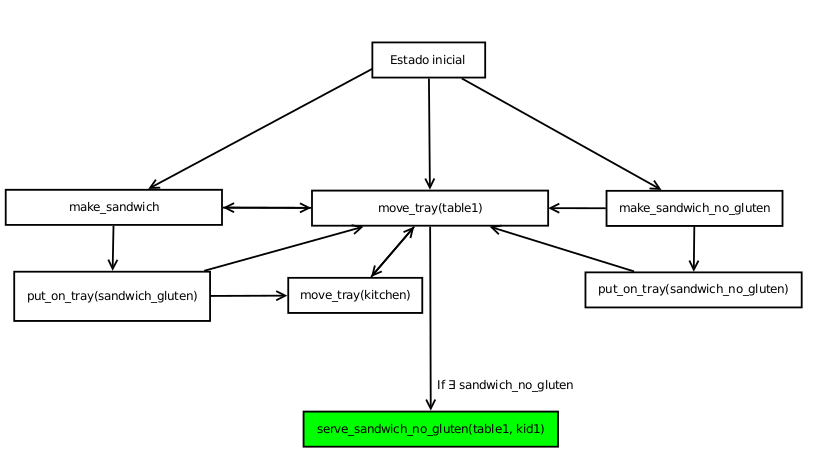
\includegraphics[width=\textwidth, height=9cm]{domain-02-1}
        \caption{Grafo de búsqueda con la versión original}
    \end{figure}
    
    \begin{figure}[H]
        \centering
        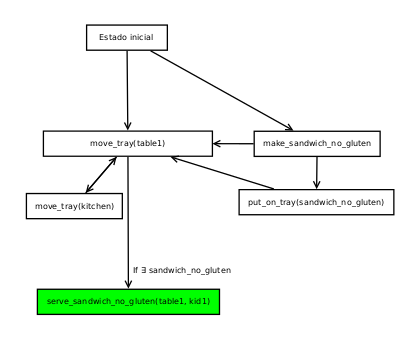
\includegraphics[width=\textwidth, height=9cm]{imgTr}
        \caption{Grafo de búsqueda con la versión 02}
    \end{figure}
    
    
    \paragraph{}
    Como se puede ver, el grafo de búsqueda de la versión 02 es un subconjunto del grafo de búsqueda del dominio original. Dicho de manera más genérica, este nuevo dominio sirve para podar el grafo de búsqueda original para el subconjunto de los problemas posibles en los que existen niños alérgicos al gluten y que por tanto con en el dominio original el planificador podría perder tiempo buscando en ramas del grafo de búsqueda que se sabe a priori que no van a conducir a la solución.
    
    \paragraph{}
    Esto quiere decir que este nuevo dominio es completo y óptimo, pues lo único que se ha hecho ha sido una poda de una rama del grafo de búsqueda que sólo conduce a soluciones erróneas.
    
    \subsubsubsection{Versión 03}
    
    \paragraph{}
    Esta versión mantiene la definición de los problemas original, variando exclusivamente la definición del dominio. Esta versión, al igual que la versión 01 se basa en la utilización de macro-operadores, pero llevando su uso hasta el extremo. En este dominio, se han implementado los macro-operadores \\ \cool{ make\_sandwich\_move\_tray\_serve\_sandwich\_move\_tray\_kitchen}, \\ \cool{make\_sandwich\_move\_tray\_serve\_sandwich\_no\_gluten\_move\_tray\_kitchen} y \\ \cool{move\_tray\_kitchen} que sustituirían a todos los demás operadores. Como se ha mencionado en la versión 01, al ser esta una versión que utiliza macrooperadores, hace uso también de la función numérica con dígitos \cool{total\_cost}, incrementando su coste en cuatro unidades tras la ejecución de los dos macrooperadores y en uno al ejecutar el operador \cool{move\_tray\_kitchen}. La lógica subyacente a la inclusión de esta función es idéntica que en el caso de la versión 01; en la sección que se explica esta versión se puede encontrar también la explicación de la utilización de \cool{total\_cost}.
    
    \paragraph{}
    Volviendo a los operadores, los dos primeros tendrían como precondiciones que existiese al menos un componente y un trozo de pan con o sin gluten (según cuál de los dos operadores sea), que haya una bandeja en la cocina y que exista un niño alérgico o no al gluten (igualmente, según el operador que corresponda) esperando a ser servido. En caso de que se dé este supuesto, estos operadores producirían un sándwich, lo cargarían en una bandeja, lo transportarían hasta donde está el niño, servirían al niño y traerían la bandeja de vuelta a la cocina. Por otro lado, en caso de que no haya ninguna bandeja en la cocina en el estado inicial, se ejecutaría el operador \cool{move\_tray\_kitchen}.
    
    \paragraph{}
    Este macrooperador reduce el árbol de búsqueda en tanto que existen únicamente tres operadores que se pueden utilizar. Sin embargo, el árbol de búsqueda contiene un estado por cada instancia posible del operador, valor directamente proporcional al número de parámetros de entrada de dicho operador, que en este caso es muy elevado. La relación entre la pérdida de estados del árbol de búsqueda debido a la disminución de operadores encapsulados en nuevos macro-operadores y la ganancia de estados en el árbol de búsqueda debido al incremento de instancias del nuevo operador se llama utilidad y será analizada en la sección de resultados de ejecución.
    
    \paragraph{}
    Si no se incluyesen los operadores originales, esta versión sería completa pero no óptima, puesto que no se podría servir a más de un niño sin tener que pasar por la cocina. Por tanto, en esta versión se conservan los operadores originales para no perder la optimalidad.
    
    \subsubsubsection{Versión 05}
    
    \paragraph{}
    En esta versión, varía tanto la definición del problema como la definición del dominio. Se trata de un dominio numérico con proposiciones, en las que se definen de manera numérica el número de panes, contenidos, sándwiches con y sin gluten. Los niños no son definidos de manera numérica ya que en la definición original en la meta se especifica los niños concretos (con su respectiva localización) que deben ser servidos, por lo que si fuesen definidos de manera numérica los niños servidos con un operador como \cool{served\_childs ?num - num} se perdería esta capacidad para especificar no sólo el número sino los niños concretos dentro de todos los definidos en el problema que deben ser servidos para la correcta resolución del problema. Existe sin embargo la posibilidad de hacer contadores que incluyan a los niños pero estos planes deben después ser post-procesados. Sin ir más lejos, esto se puede lograr con \textit{Baggy}.
    
    \paragraph{}
    Los nuevos predicados utilizados son: \\ \cool{(at\_kitchen\_bread ?gluten - num ?no-gluten - num)},  \cool{(at\_kitchen\_content ?gluten - num ?no-gluten - num)}, \\ \cool{(at\_kitchen\_sandwich ?gluten - num ?no-gluten - num)} y \cool{(ontray ?gluten - num ?no-gluten - num ?t - tray)} que definen respectivamente el número de panes, contenidos y sándwiches en la cocina y los sándwiches que se encuentran en las bandejas que tengan o no gluten. A su vez, se ha añadido el predicado \cool{(next ?minor - num ?major - num)} que sirve para incrementar y decrementar en una unidad los valores numéricos de los predicados definidos anteriormente. Los predicados del dominio original \cool{(allergic\_gluten ?c - child)}, \cool{(not\_allergic\_gluten ?c - child)}, \cool{(waiting ?c - child ?p - place)}, \cool{(at ?t - tray ?p - place)} y \cool{(served ?c - child)} se han mantenido.
    
    \paragraph{}
    Aunque la apariencia es totalmente distinta, la lógica de los operadores es la misma que en el caso original pero adaptada a estas nuevas definiciones numéricas con proposiciones. Únicamente ha sido necesario incluir el operador \\ \cool{make\_sandwich\_bread\_no\_gluten} y \cool{make\_sandwich\_content\_no\_gluten} que crea sándwiches con gluten con el pan o el contenido sin gluten.
    
    \paragraph{}
    Los operadores numéricos comprueban la existencia de lo que serían los parámetros necesarios en el dominio original no a través de la comprobación de la existencia de por ejemplo el nuevo parámetro \cool{(at\_kitchen\_bread ?gluten - num ?no-gluten - num)}, pues siempre va a existir, sino de los valores numéricos contenidos en estos parámetros que en este caso determinan cuántos panes con y sin gluten existen en la cocina. Es decir, en la definición del nuevo problema se definen la lista de sucesión de valores numéricos mediante parámetros como \cool{(next number\_0 number\_1)} o \cool{(next number\_1 number\_2)}, lo que permite tanto sumar y restar una unidad como saber cuál es el menor valor posible que se puede definir (en este caso, el cero). Así, la comprobación que habría que hacer en este dominio para poder decrementar o incrementar un valor de un parámetro es si existe dicho sucesor o predecesor de dicho valor entre las definiciones del problema. Si no tienes predecesor de un número por ejemplo, sabes que el valor que tiene es cero.
    
    \paragraph{}
    Para que esto se entienda mejor se va a explicar el funcionamiento de uno de los operadores, por ejemplo de \textit{make\_sandwich\_no\_gluten}. Las precondiciones que tiene este operador son que existan los hechos \cool{(at\_kitchen\_bread ?bread-gluten ?bread-no-gluten)}, \\ \cool{(at\_kitchen\_content ?content-gluten ?content-no-gluten)} y \\ \cool{(at\_kitchen\_sandwich ?sandwich-gluten ?sandwich-no-gluten)}, que exista el predecesor del pan y el contenido para saber que existe al menos una unidad de cada uno de los componentes que se van a utilizar \cool{(next ?bread-no-gluten-minor ?bread-no-gluten)} y \cool{(next ?content-no-gluten-minor ?content-no-gluten)} y que exista el sucesor del sándwich que se va a generar para que se pueda incrementar el número de sándwiches \\ \cool{(next ?sandwich-no-gluten ?sandwich-no-gluten-major)}. El número máximo de sándwiches por tanto está definido por el mayor número definido en un parámetro \cool{(next ?n ?maximo)}, siendo el valor de \cool{?maximo} el número de cláusulas \textit{notexist} del problema original. Finalmente, este operador elimina los hechos \cool{(at\_kitchen\_bread ?bread-gluten ?bread-no-gluten)}, \\ \cool{(at\_kitchen\_content ?content-gluten ?content-no-gluten)} y \\ \cool{(at\_kitchen\_sandwich ?sandwich-gluten ?sandwich-no-gluten)} mediante la negación de los mismos en los efectos de este operador para así poder incrementar o decrementar sus valores \cool{?bread-no-gluten}, \cool{?content-no-gluten} y \\ \cool{?sandwich-no-gluten-major)}). Es decir, con los hechos definidos inicialmente el el problema \cool{(next ?num ?numPlusOne)} se obtiene la escala de valores cuantitativos, pero al no ser esta definición numérica con dígitos, no es posible modificar los hechos para incrementar o decrementar su valor si no es mediante el borrado del hecho inicial y la declaración de un nuevo hecho que contenga el nuevo valor. 
    
    \paragraph{}
    Por último, esta solución es completa y óptima, puesto que es una redefinición de los operadores originales para adaptarlos a la lógica de un dominio numérico con proposiciones que sin embargo conserva por completo la lógica inicial del problema, por lo que a diferencia de otras versiones como en la 01 en que es necesario conservar los operadores originales para no perder la optimalidad, en este caso no es necesario, pues todas las acciones del dominio original se pueden realizar de manera atómica en este dominio (a diferencia de lo que ocurre con los dominios que usan macro-operadores, que es necesario aplicar varias acciones de las acciones agrupadas en el nuevo dominio para la aplicación de acciones individuales del dominio original). A continuación se incluye la definición de uno de los problemas.
    
    \subsubsubsection{Dominio 08}
    \paragraph{}
    Esta versión sería la equivalente realizada a mano a la versión del dominio numérico con dígitos generado automáticamente. A diferencia de lo que ocurre con las versiones numéricas con palabras, en este caso la representación generada automáticamente y la representación manual son muy similares. De hecho, los nombres de los predicados utilizados en esta versión han sido cambiados para que coincidiesen con los obtenidos en la versión automática ya que de esta manera ambas versiones tienen una representación común de los problemas. Respecto a la representación del dominio, existen algunas variaciones tanto en relación con la versión numérica con palabras realizada a mano como con la versión automática numérica con dígitos.
    
    \paragraph{}
    En relación con la versión 05 del problema, el número de acciones, sus precondiciones y efectos son idénticos. Lo único que cambia entre ambas versiones es que la representación numérica de los predicados en este caso es con dígitos y en el anterior es con palabras.
    
    \paragraph{}
    Respecto al dominio numérico con dígitos generado automáticamente, lo único que varía entre ambos es que en el dominio automático se ha fragmentado en dos operadores el operador de este dominio \cool{serve\_sandwich\_no\_gluten}. Este operador sirve indistintamente un sándwich sin gluten a niños alérgicos al gluten y a niños no alérgicos al gluten, puesto que se ha eliminado de las precondiciones del operador si el niño es alérgico o no al gluten. Por otro lado, en el dominio generado automáticamente este operador ha sido dividido en otros dos al incluir en las precondiones si el niño es o no alérgico al gluten, teniendo por tanto un operador para cada uno de estos dos supuestos.
    
    \subsubsubsection{Dominio 09}
    
    \paragraph{}
    En esta versión se modifican tanto los problemas como el dominio. La modificación realizada consiste en eliminar el parámetro \cool{(waiting ?c - child ?p - place)} para incluir la posición de los niños en \cool{(allergic\_gluten ?c - child ?p - place)} y \cool{(not\_allergic\_gluten ?c - child ?p - place)}. La idea de esta modificación es que los parámetros \cool{waiting} y \cool{allergic\_gluten} o \\ \cool{not\_allergic\_gluten} siempre aparecen juntos en los mismos operadores para referirse al mismo valor de \cool{child}, por lo que con esta modificación se intenta comprobar si este tipo de uniones de parámetros cuyo uso coincide en los mismos operadores reduce o no el tiempo de búsqueda.
    
    \paragraph{}
    Los únicos operadores que ha sido necesario modificar son \cool{serve\_sandwich} y \\ \cool{serve\_sandwich\_no\_gluten}, sustituyendo \cool{(waiting ?c ?p)} y \cool{(allergic\_gluten ?c)} o \cool{(not\_allergic\_gluten ?c)} por los nuevos parámetros \cool{(allergic\_gluten ?c - child ?p - place)} y \cool{(not\_allergic\_gluten ?c - child ?p - place)}. A continuación se incluye un problema definido para esta versión.
    
    \paragraph{}
    Esta versión es completa y óptima puesto que sólo se ha cambiado la representación de los parámetros de algunos operadores pero no se ha modificado la funcionalidad original de los mismos.
    
    \subsubsubsection{Dominio 11}
    
    \paragraph{}
    Esta versión requiere de la modificación de tanto los dominios como de los problemas, y la modificación consiste en eliminar el predicado \cool{(not\_allergic\_gluten ?c - child)} para tratarlo en los operadores como la negación del predicado \\ \cool{(allergic\_gluten ?c - child)}, es decir, como \cool{(not(allergic\_gluten ?c - child))}. Esto implica eliminar en los problemas los parámetros \cool{(allergic\_gluten ?c - child)} y modificar únicamente el operador \cool{serve\_sandwich} para definir al niño no alérgico al gluten que se le va a servir el sándwich de la manera que se ha decrito en la oración anterior. Un ejemplo de problema definido de esta forma sería el siguiente.
    
    \paragraph{}
    Esta versión es completa y óptima, puesto que es un cambio en la representación de la lógica, pero permanece la lógica de la versión original.
    
    \subsubsubsection{Dominio 12}
    
    \paragraph{}
    Esta es con diferencia la versión con mayor conocimiento del dominio. Para la creación de este dominio se ha buscado el método resolutivo que permite obtener siempre la solución óptima para cualquier tipo de problema de entrada para después crear una versión de los dominios y problemas que se acercase lo máximo posible a esta solución. A continuación se  encuentra el algoritmo de resolución óptimo para cualquier tipo de problema.
    
    \begin{enumerate}
        \item Contar el número de niños a los que hay que servir que son alérgicos al gluten y guardar ese valor en \textit{a}.
        \item Contar el número de niños a los que hay que servir que no son alérgicos al gluten y guardar ese valor en \textit{b}.
        \item Hacer \textit{a} sándwiches sin gluten.
        \item Hacer \textit{b} sándwiches con o sin gluten.
        \item Si no existe ninguna bandeja en la cocina, mover una bandeja a la cocina \textit{c}.
        \item Mover (\textit{a} + \textit{b}) sándwiches a la misma bandeja \textit{c}.
        \item Para cada localización \textit{d} en la que exista al menos un niño que tiene que ser servido:
        \begin{enumerate}
            \item Mover la bandeja \textit{c} a \textit{d}.
            \item Para cada niño \textit{e} que se encuentre en \textit{d} y no haya sido servido:
            \begin{enumerate}
                \item Servir el sándwich correspondiente (según sea o no alérgico al gluten) al niño \textit{e} en \textit{d} de la bandeja \textit{c}. 
            \end{enumerate}
        \end{enumerate}
    \end{enumerate}
    
    \paragraph{}
    En esta versión se ha conseguido replicar este algoritmo realizando las modificaciones en el dominio original que se expresan a continuación.
    
    \paragraph{}
    En cuanto a los \textbf{predicados}, el único predicado que se ha suprimido es \cool{(notexist ?s - sandwich)}, ya que su función es limitar el número de sándwiches que se pueden producir y este concepto ya está incluído en los nuevos predicados \\ \cool{(num\_sandwich\_no\_gluten ?n - num)} y \cool{(num\_sandwich\_gluten ?n - num)}. Estos dos predicados son parámetros introducidos por el usuario con el número de sándwiches (definidos en numérico con proposiciones) con y sin gluten que es necesario hacer y que debe coincidir con el número de niños alérgicos o no al gluten que deben ser servidos. Ambos parámetros no sólo limitan el número de sándwiches que se pueden hacer, ya que en los operadores de creación de sándwiches se verifica que el número de sándwiches restante de cada tipo sea mayor que cero, sino que también limitan los sándwiches con gluten que se pueden hacer y permiten separar los operadores en varias fases, impidiendo por ejemplo que se mueva una bandeja si antes no se han creado todos los sándwiches con y sin gluten que son necesarios. A su vez, se han incluido los predicados \cool{(next ?minor - num ?major - num)}, que sirve para la creación de variables numéricas con proposiciones tal y como se especifica en el dominio 05, \cool{(not\_trays\_kitchen)} es simplemente un operador creado para suplir la ausencia de comparaciones de tipo \cool{forall} en \textit{PDDL}, que permitiría saber si existen bandejas en la cocina y que en caso de que la posición inicial de ninguna de las bandejas esté en la cocina, será necesario añadir este predicado en el problema para indicar al dominio que es necesario ejecutar el operador \cool{move\_tray\_kitchen}. El predicado \cool{(first\_load)} se incluye siempre en la definición del problema y sirve para poder saber cuándo se ha realizado la primera carga ya que así a partir de la segunda carga se va a exigir que la bandeja en la que se cargue el sándwich ya contenga al menos un sándwich (consiguiendo con ello que todos los sándwiches se carguen en la misma bandeja, ya que el operador para la primera carga \cool{put\_on\_tray\_first\_load} que permite cargar el sándwich en cualquier bandeja sólo se va a poder ejecutar una única vez). Finalmente, el predicado \cool{(num\_sandwich\_ontray ?n - num)} es inicializado con el número de sándwiches totales con y sin gluten que tienen que realizarse para así poder disminuir en una unidad cada sándwich cargado en la bandeja para que así se pueda poner como limitador de movimiento de las bandejas que ninguna se puede mover hasta que estén cargados todos los sándwiches.
    
    \paragraph{}
    Como en esta versión se han realizado importantes modificaciones en los \textbf{operadores}, por lo que van a ser explicados uno a uno como se realizó en el dominio original.
    
    \begin{itemize}
        \item \textbf{make\_sandwich\_no\_gluten (porción de pan sin gluten, porción de contenido sin gluten, número de sándwiches actuales sin gluten, siguiente número de sándwiches sin gluten)}
            \begin{itemize}
                \item \textbf{Precondiciones}: que exista al menos un contenido y un trozo de pan donde ambos sean sin gluten y exista un predecesor del número de sándwich sin gluten por hacer.
                \item \textbf{Efectos}: eliminación de los dos componentes utilizados, decremento del número de sándwiches sin gluten que quedan por hacer y creación de un sandwich sin gluten.
            \end{itemize}
        \item \textbf{make\_sandwich (porción de pan, porción de contenido, número de sándwiches actuales con gluten, siguiente número de sándwiches con gluten)}
            \begin{itemize}
                \item \textbf{Precondiciones}: que exista al menos un contenido y un trozo de pan donde cualquiera o ambos de ellos pueden contener o no gluten, que exista un predecesor del número de sándwich con gluten por hacer y que se hayan hecho todos los sándwiches necesarios sin gluten.
                \item \textbf{Efectos}: eliminación de los dos componentes utilizados, decremento del número de sándwiches con gluten que quedan por hacer y creación de un sandwich etiquetado como con gluten.
            \end{itemize}
        \item \textbf{move\_tray\_kitchen (bandeja portátil, posición inicial, hecho auxiliar)}
            \begin{itemize}
                \item \textbf{Precondiciones}: que exista el hecho que indica que no hay ninguna bandeja en la cocina y se hayan hecho todos los sándwiches con y sin gluten que había que hacer.
                \item \textbf{Efectos}: mueve una bandeja a la cocina y eliminación del hecho que indica que no hay ninguna bandeja en la cocina para que así no se pueda repetir esta acción con más bandejas y así se pierda la optimalidad.
            \end{itemize}
        \item \textbf{put\_on\_tray\_first\_load (número de sándwiches en la cocina, bandeja que se encuentra en la cocina, número de sándwiches en la bandeja anterior, hecho de que es la primera carga)}
            \begin{itemize}
                \item \textbf{Precondiciones}: que se hayan hecho todos los sándwiches con y sin gluten que había que hacer, que haya al menos una bandeja en la cocina y que sea la primera carga en una bandeja.
                \item \textbf{Efectos}: carga en una bandeja un sándwich.            
            \end{itemize}
        \item \textbf{put\_on\_tray (número de sándwiches en la cocina, bandeja que se encuentra en la cocina, número de sándwiches en la bandeja anterior, hecho de que no es la primera carga)}
            \begin{itemize}
                \item \textbf{Precondiciones}: que se hayan hecho todos los sándwiches con y sin gluten que había que hacer, que haya al menos una bandeja en la cocina y que la bandeja sobre la que se va a cargar tenga ya al menos un sándwich.
                \item \textbf{Efectos}: carga un sándwich en una bandeja previamente cargada.
            \end{itemize}        
        \item \textbf{move\_tray (bandeja, posición inicial, hecho de que se han cargado todos los sándwiches, posición niño en espera no alérgico al gluten)}
            \begin{itemize}
                \item \textbf{Precondiciones}: que se hayan hecho todos los sándwiches que había que hacer con y sin gluten, que se hayan cargado todos los sándwiches en la bandeja y que en la posición actual no quede ningún niño al que se le pueda servir un sándwich con gluten.
                \item \textbf{Efectos}: mueve la bandeja a una nueva posición.
            \end{itemize}                
        \item \textbf{move\_tray\_no\_gluten (bandeja, posición inicial, hecho de que se han cargado todos los sándwiches, posición niño en espera alérgico al gluten)}
            \begin{itemize}
                \item \textbf{Precondiciones}: que se hayan hecho todos los sándwiches que había que hacer con y sin gluten, que se hayan cargado todos los sándwiches en la bandeja y que en la posición actual no quede ningún niño al que se le pueda servir un sándwich sin gluten.
                \item \textbf{Efectos}: mueve la bandeja a una nueva posición.
            \end{itemize}                
        \item \textbf{serve\_sandwich\_no\_gluten (niño no alérgico al gluten, niño esperando, posición niño, posición bandeja)}
            \begin{itemize}
                \item \textbf{Precondiciones}: que al menos una de las bandejas portátiles esté en la misma posición que uno de los niños, que la bandeja que cumpla la precondición anterior tenga al menos un sándwich sin gluten, que un niño no alérgico al gluten esté en la misma localización que la bandeja que cumple las precondiciones anteriores y que este mismo niño esté esperando un sándwich.
                \item \textbf{Efectos}: el niño pasa a estar servido y se elimina el sándwich utilizado en la operación.
            \end{itemize}
        \item \textbf{serve\_sandwich (niño alérgico al gluten, niño esperando, posición niño, posición bandeja)}
            \begin{itemize}
                \item \textbf{Precondiciones}: que al menos una de las bandejas portátiles esté en la misma posición que uno de los niños, que la bandeja que cumpla la precondición anterior tenga al menos un sándwich con o sin gluten, que un niño no alérgico al gluten esté en la misma localización que la bandeja que cumple las precondiciones anteriores y que este mismo niño esté esperando un sándwich.
                \item \textbf{Efectos}: el niño pasa a estar servido y se elimina el sándwich utilizado en la operación.
            \end{itemize}
    \end{itemize}
    
    
    
    \subsection{Versiones generadas automáticamente}
    \paragraph{}
    En esta sección se explicará brevemente la composición de las versiones generados automáticamente mediante software independiente de dominio de terceros. Para todos estos dominios se ha utilizado exclusivamente como entrada el problema y el dominio original.
    
    \paragraph{}
    Como la lógica de estas modificaciones es de otros propietarios, las explicaciones serán bastante menos detalladas que las que aparecen en la sección de los dominios modificados a mano.
    
    \subsubsection{Versión PTT}
    \paragraph{}
    Este modificador debería transformar el dominio mediante la inclusión de macrooperadores, que como se ha mostrado en la sección de dominios hechos a mano, existen varias alternativas para dicha implementación. Sin embargo, el software de \textit{PTT} ha sido incapaz de encontrar un solo macrooperador, por lo que tanto la definición del dominio como los problemas generados son los mismos que los introducidos como entrada, por lo que en lo referente a la comparación de los tiempos obtenidos con las distintas versiones esta versión de los problemas va a ser descartada, al ser exactamente igual que la versión original del problema.\footnote{En ejecuciones de este software con otras versiones de este dominio, se ha comprobado que este software es capaz de encontrar macrooperadores. Sin embargo, al centrar el estudio en la comparación de las distintas versiones que tienen como punto de partida el dominio original, estas modificaciones han sido descartadas.}
    
    \subsubsection{Versión numérica con proposiciones}
    \paragraph{}
    Esta versión ha sido generada automáticamente mediante el software \textit{Baggy}, que transforma los dominios en representaciones numéricas con proposiciones. Baggy añade una gran cantidad de predicados que hacen difícil de seguir su lógica para explicar en detalle su motivación, como es el caso cuando tiene por entrada el dominio y los problemas originales. Respecto a las acciones, estas incororan estos nuevos predicados tanto en las precondiciones como en los efectos así como también sucede tanto en la inicialización como en los efectos de los problemas.
    
    \paragraph{}
    Por último, al ser únicamente un cambio de representación, los operadores iniciales han sido conservados no así los predicados que estos contenían.
    
    \subsubsection{Versión numérica con dígitos}
    \paragraph{}
    Esta versión modifica la representación del dominio para que sea numérica con dígitos. Respecto a la versión modificada a mano que es también numérica con dígitos, la representación de los problemas es la misma puesto que se han cambiado el nombre de los predicados de la versión manual para que así sea. En lo que atañe al dominio, todos los operadores son idénticos entre sí entre ambas versiones a excepción del operador para servir sándwiches sin gluten. Mientras que en la versión manual se ha quitado de las precondiciones si el niño que va a recibir el sándwich es alérgico o no para que así este operador sea válido para los dos casos, en el caso de la versión generada automáticamente este operador se ha desglosado en dos incluyendo en cada uno la precondición de si el niño que va a recibir el sándwich es alérgico o no al gluten.
    
    \paragraph{}
    Este desdoblamieto de operadores respecto al dominio generado a mano no aporta ningún beneficio, ya que el hecho de que el niño sea o no alérgico al gluten se encuentra en ambos casos exclusivamente en las precondiciones y no en los efectos. Es decir, se está incrementando respecto a la versión hecha a mano el número de precondiciones de un operador así como se está añadiendo un nuevo operador innecesario, siendo el resto de operadores idénticos entre ambas versiones (y que por ello no van a volver a ser explicados). Esta modificación por tanto incrementa el factor de ramificación sin ninguna contrapartida, por lo que por lo menos el tiempo de búsqueda debería ser igual o mayor que la versión manual. Esta hipótesis será comprobada experimentalmente en la sección de evaluación de resultados.
    
    \pagebreak
    
    \section{Resultados obtenidos}
    \paragraph{}
    En esta sección se van a detallar las pruebas realizadas así como los resultados obtenidos con su correspondiente interpretación. La tendencia de estos resultados debería ser la misma independientemente de las características del hardware y del sistema operativo utilizado, sin embargo los resultados absolutos varían según estas dos características, motivo por el cual se incluyen estos datos.
    
    \paragraph{}
    Todas las pruebas a las que se va a mentar en esta sección son pruebas de eficiencia de los distintos planificadores con las distintas versiones de los problemas. No se ha realizado ninguna prueba funcional para comprobar la correctitud de los scripts ya que resulta más fiable y requiere menos tiempo verificar que el resultado de alguna prueba aleatoria de su ejecución coincide con la ejecución manual que diseñar pruebas funcionales que verifiquen lo que ya se ha hecho a mano.
    
    \subsection{Especificaciones del ordenador utilizado}
    \paragraph{}
    Como ya se ha comentado, el hardware y el sistema operativo utilizado influyen en los resultados obtenidos en las pruebas de eficiencia realizadas. Por este motivo, se incluye a continuación estas características.
    
    \begin{itemize}
        \item Tipo de dispositivo: ordenador de sobremesa
        \item Modelo: Hewlett Packard 550-244NS A\footnote{https://support.hp.com/es-es/document/c05045080}
        \item Procesador: AMD A10 8750 
        \item Frecuencia: 3.6GHz
        \item Memoria RAM: 16GB
        \item Sistema operativo: GNU-Linux Debian 8.7
    \end{itemize}
    
    \subsubsection{Planificadores utilizados}
    \paragraph{}
    Los planificadores utilizados para las pruebas realizadas son \textit{Metric-FF} en su versión 2.1 y \textit{LPG} en su versión \textit{td}. Inicialmente también se incluyó el planificador FastDownward utilizando Lama2011 como heurística, pero se descartó este planificador al resolver menos del 10\% del total de problemas para todas las versiones por debajo de los 30 minutos de tiempo límite de búsqueda del planificador por cada problema, lo que impide poder extraer conclusiones sólidas de la mejora entre las distintas representaciones de los problemas. Por otro lado, con los dos planificadores utilizados para estas pruebas el 100\% de los problemas de alguna de esas versiones eran resueltos en su totalidad por ambos planificadores.. El funcionamiento interno de estos tres planificadores queda descrito en la sección del estado del arte.
    
    \paragraph{}
    Podría haberse aumentado el número de planificadores utilizados para la sección de pruebas. Sin embargo, teniendo en cuenta que una estimación muy benévola de la sección de planificación del proyecto se estimaba el número de horas de ejecución de las pruebas funcionales en 139 horas de ejecución, la inclusión de pruebas con nuevos planificadores implicarían un gasto de tiempo considerable. Si se hubiese dispuesto de más tiempo, se podrían haber incluído pruebas con más planificadores. Estas pruebas posteriores se cree que podrían haber servido para entender la relación de las modificaciones realizadas con un entorno más amplio de planificadores para así quizá poder sacar conclusiones apriorísticas sobre el tipo de modificaciones que pueden beneficiar a un tipo concreto de planificador. Esto por falta de tiempo no ha podido ser realizado por lo que se encuentra entre las líneas de trabajo por las que se podría continuar este proyecto.
    
    \paragraph{}
    Existe también otra alternativa que es realizar las pruebas exclusivamente con un único planificador. Esta opción podría hacer que se extrajesen conclusiones equivocadas o muy limitadas respecto a las modificaciones realizadas en los dominios, puesto que la mejora en la planificación que se puede obtener con dichas modificaciones depende del planificador y de la heurística que éste utilice.
    
    \paragraph{}
    Los parámetros de ejecución utilizados para estos planificadores son:
    
    \begin{itemize}
        \item \textbf{Metric-FF}: -s 0 (\textit{FF} estándar: \textit{EHC+H} y \textit{BFS}).
        \item \textbf{LPG-td}: -n 1 (genera únicamente una solución).
    \end{itemize}
    
    \paragraph{}
    Respecto al coste de las acciones, la ejecución de las acciones de todas las versiones tienen coste 1 salvo en el caso de los dominios con macrooperadores, en cuyo caso los macrooperadores tienen el coste del número de operadores del dominio original que estén sustituyendo.
    
    \subsubsection{Métricas utilizadas}
    \paragraph{}
    Los problemas han sido ejecutados por cada planificador con un tiempo máximo de 30 minutos por cada problema, que es el tiempo límite utilizado en las competiciones de la \textit{IPC}. En caso de no encontrar una solución en ese lapso de tiempo, el problema contabiliza como no resuelto.
    
    \paragraph{}
    Las métricas utilizadas para la comparación de los resultados han sido estas tres:
    \begin{itemize}
        \item Tiempo necesario para encontrar la solución.
        \item Longitud del plan (en caso de encontrar solución).
        \item Calidad relativa de la solución según la métrica de la \textit{IPC}.
    \end{itemize}
    
    
    \subsection{Pruebas realizadas}
    \paragraph{}
    Las pruebas que se han realizado tenían como fin demostrar una hipótesis surgida de una mezcla de intuición y de la revisión del estado del arte: que tanto el tiempo de búsqueda de un planificador como la calidad de la solución de un mismo problema podía variar con la modificación de la representación del dominio y/o del problema. El software utilizado de otros investigadores que ha sido utilizado para estas pruebas, como se explicó en la sección de la solución propuesta, tiene sus limitaciones y no es capaz de encontrar siempre las mejores modificaciones que por otra parte sí son posibles encontrar a mano. Esto es algo que intuitivamente era de esperar. En esta sección se intentará cuantificar el coste que supone la automatización de estas modificaciones.
    
    \subsection{Resultados obtenidos}
    
    \paragraph{}
    En las siguientes secciones, va a a intentar medir la calidad de cada una de las versiones para cada uno de los dos planificadores analizados en relación a estas tres métricas mencionadas en el apartado anterior.
    
    \paragraph{}
    Para evitar saturar las gráficas con demasiadas funcione que impidan ver con claridad los resultados obtenidos, se han separado las distintas versiones a comparar en grupos de 1 a 4 versiones según la similitud de los cambios realizados. A su vez, se ha incluido en todos ellos la representación de la función de la versión original para poder ver el grado de mejora o pérdida respecto a ésta.
    
    \subsubsection{Comparación de las versiones 01 y 03}
    \paragraph{}
    En esta sección, se van a comparar los resultados obtenidos al ejecutar las siguientes versiones de los problemas que se han generado utilizando macrooperadores (es decir, la versión 01 y 03 de los problemas realizados a mano).
    
    \paragraph{}
    Como ya se comentó en la sección de la solución propuesta, en esta sección no se van a incluir los tiempos de ejecución de la versión obtenida mediante las modificaciones de \textit{PTT} puesto que este software no fue capaz de realizar una sola modificación del dominio original, por lo que todos los resultados funcionales serían idénticos a los del dominio original puesto que es el mismo.
    
    \begin{figure}[H]
        \centering
        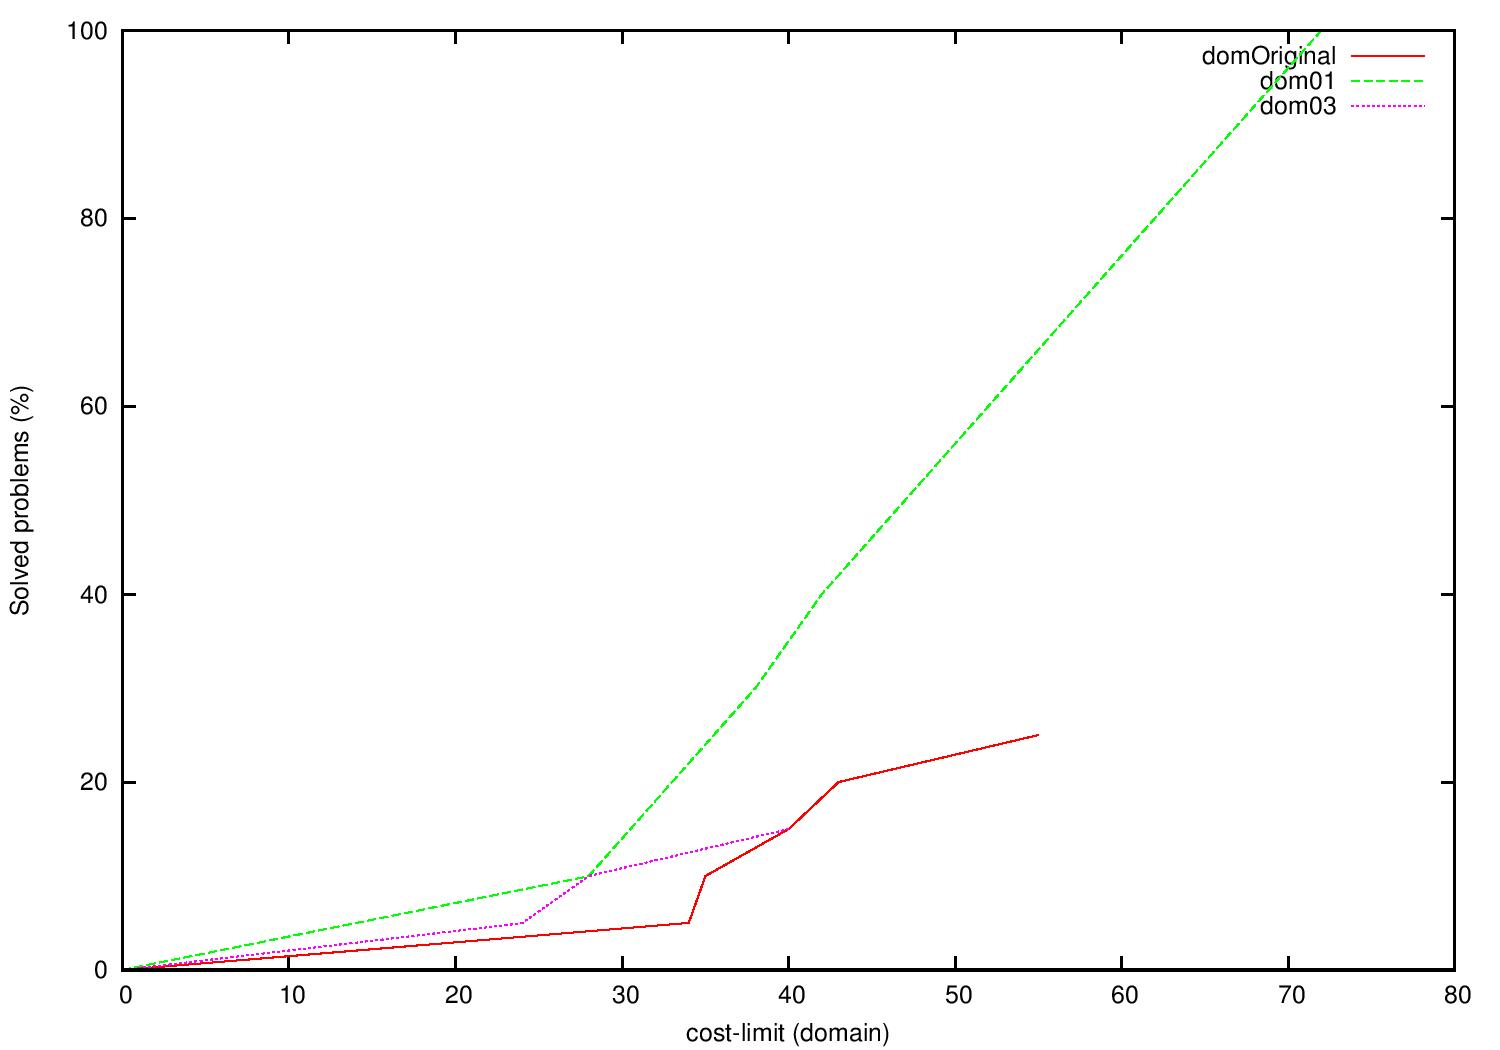
\includegraphics[width=12cm, height=8cm]{mff-or-01-03-cost}
        \caption{MFF-original-01-03-coste}
    \end{figure}
    
    \begin{figure}[H]
        \centering
        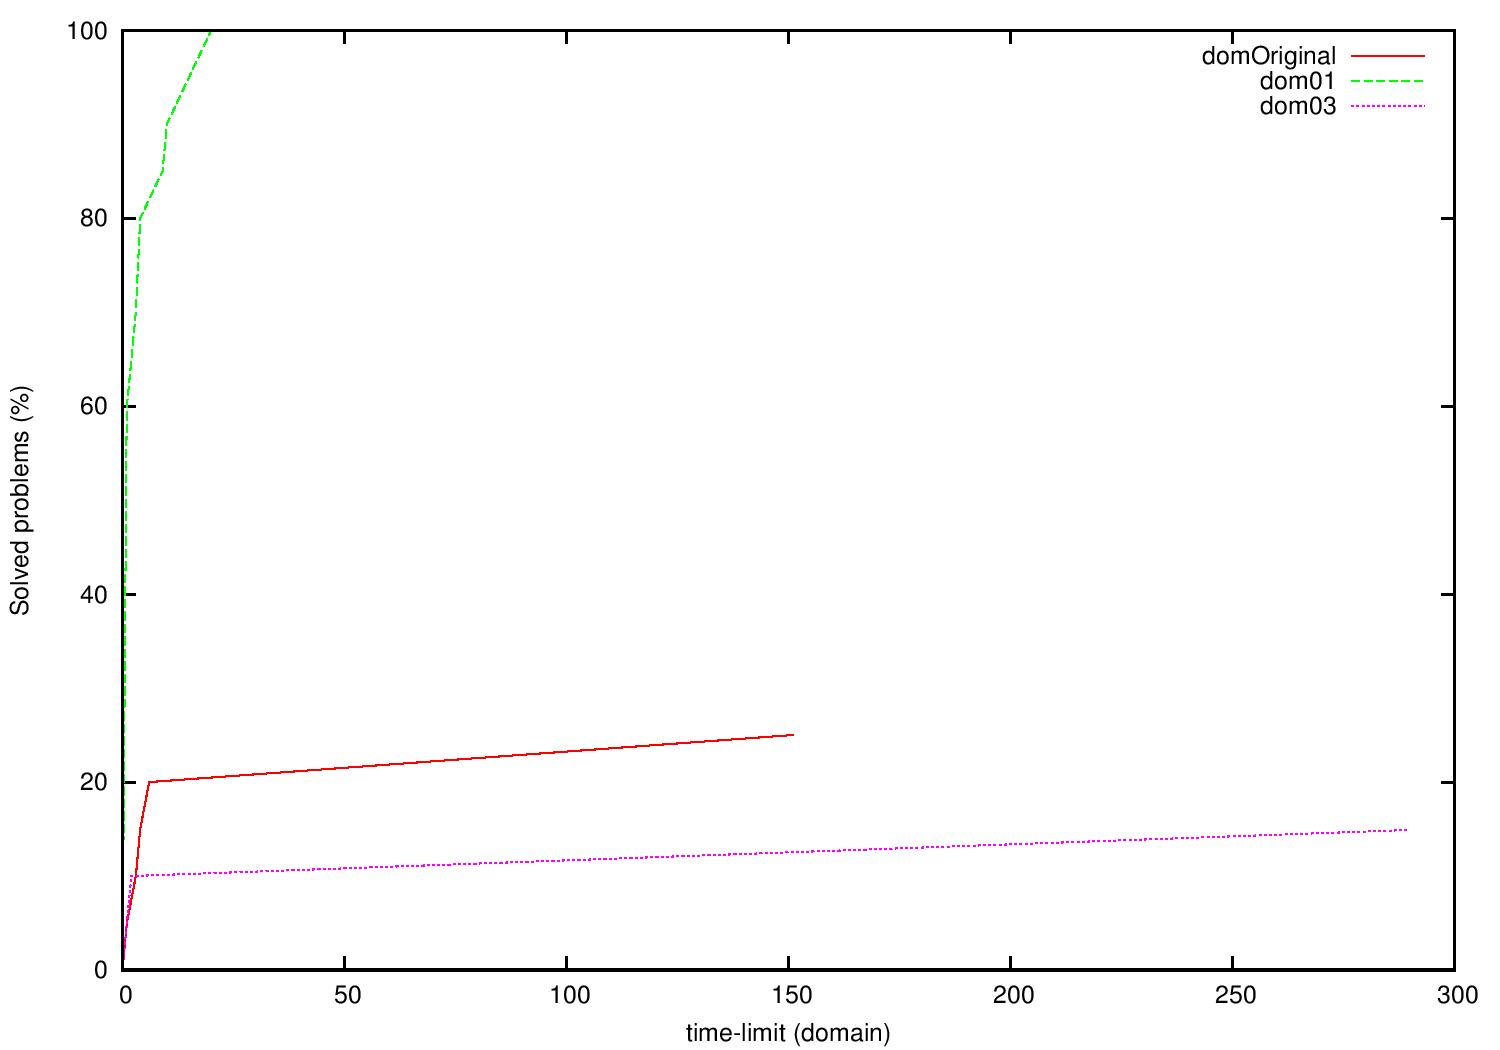
\includegraphics[width=12cm, height=8cm]{mff-or-01-03-time}
        \caption{MFF-original-01-03-tiempo}
    \end{figure}
    
    \begin{figure}[H]
        \centering
        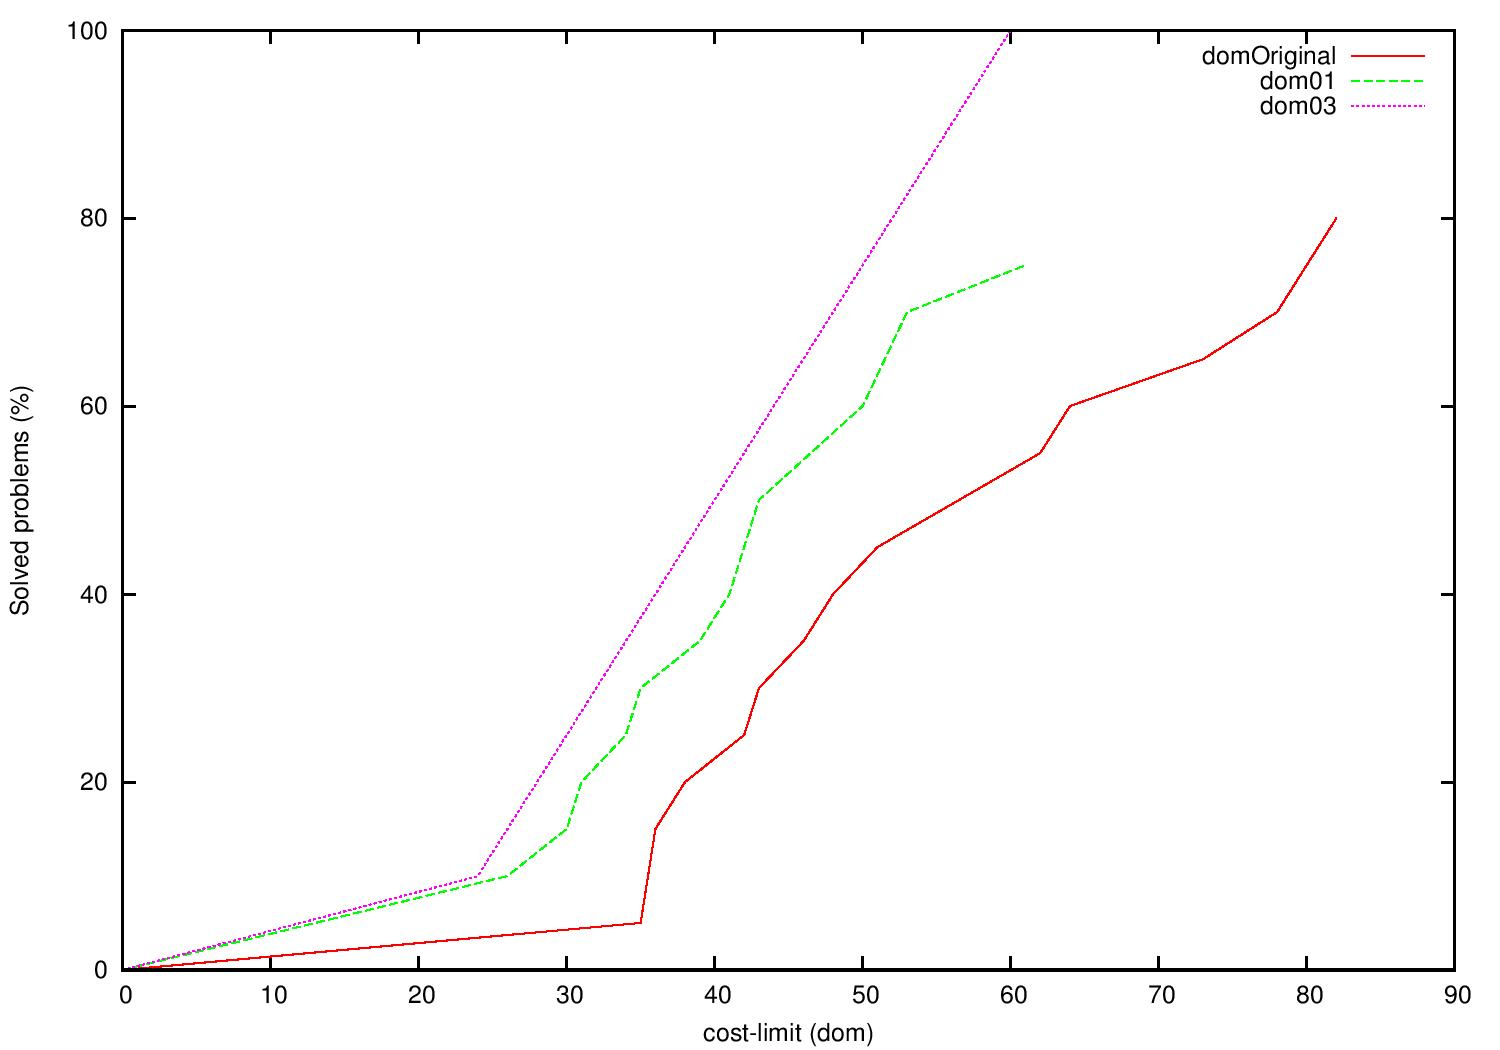
\includegraphics[width=12cm, height=8cm]{lpg-or-01-03-cost}
        \caption{LPG-original-01-03-coste}
    \end{figure}
    
    \begin{figure}[H]
        \centering
        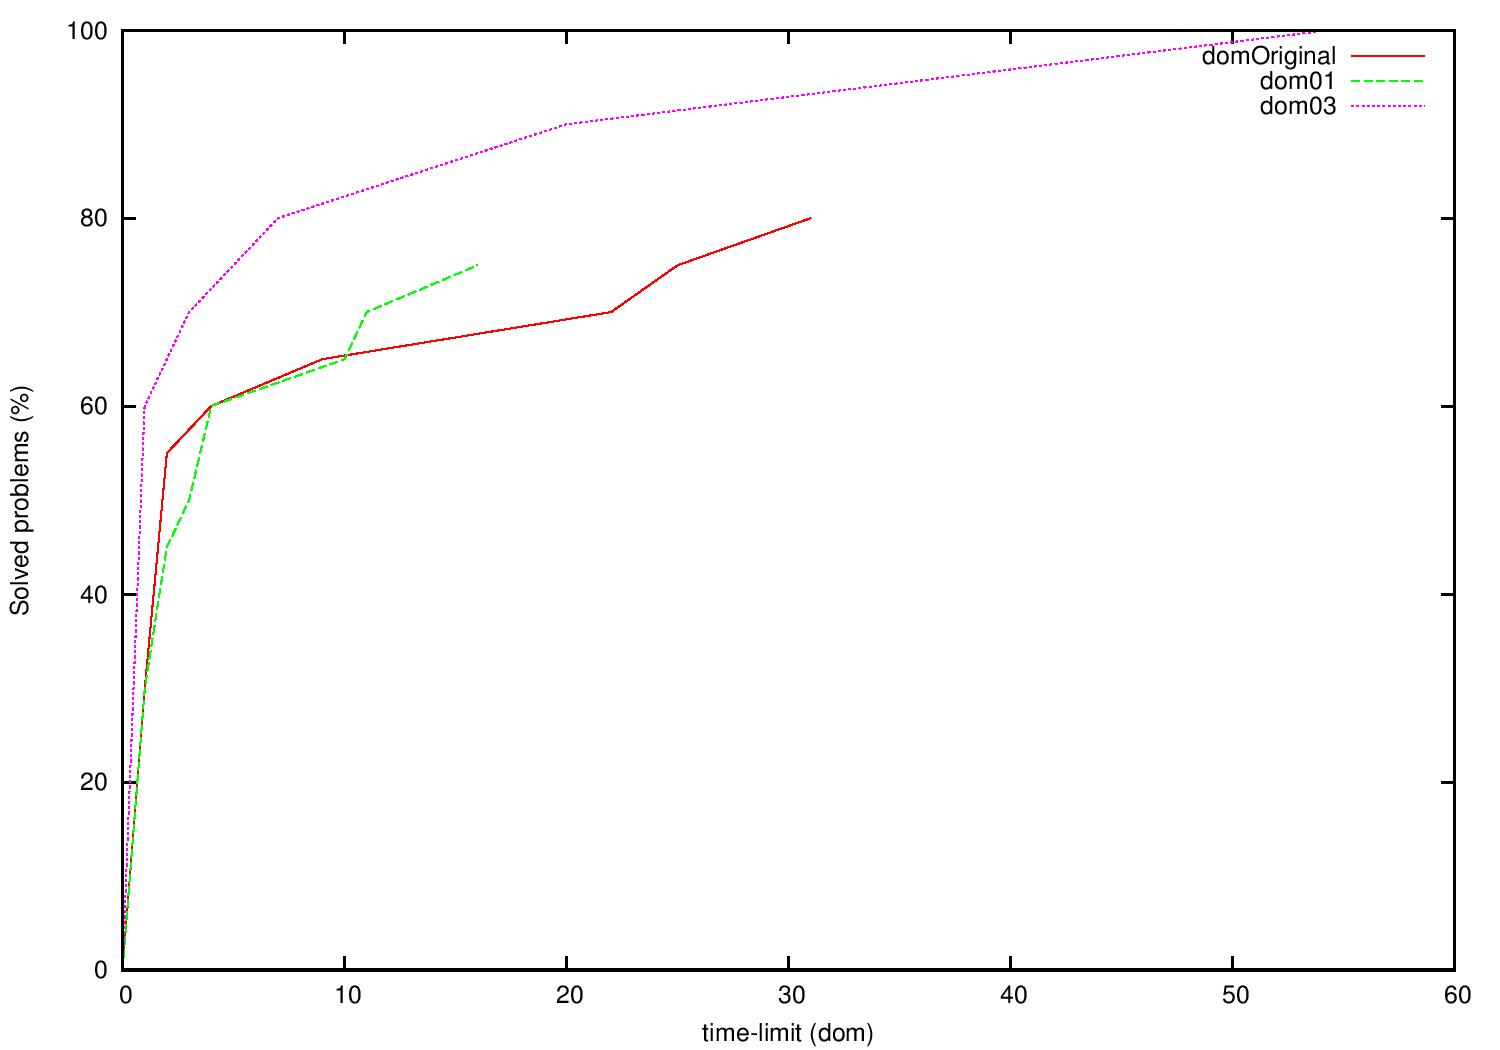
\includegraphics[width=12cm, height=8cm]{lpg-or-01-03-time}
        \caption{LPG-original-01-03-tiempo}
    \end{figure}
    
    \paragraph{}
    En los resultados obtenidos con \textit{MFF} se puede ver en la figura 4 que el coste para resolver los mismos problemas es mayor en la versión 01 que tanto en la versión original como en la versión 03. De hecho, la que tiene un menor coste de las tres es la versión original. Por otro lado, en la versión 01 consigue resolver todos los problemas, a diferencia de lo que ocurre en la versión 03 que resuelve además menos problemas que la versión original. A esto hay que añadir que el tiempo de ejecución para la resolución de los problemas es muy inferior en el caso de la versión 01 y es superior en el caso de la versión 03, tal y como se observa en la figura 5.
    
    \paragraph{}
    La interpretación que se hace de estos resultados es que mientras que en el primero la \textit{utilidad} del macrooperador está ajustada para que contrarreste los efectos negativos que produce por ejemplo un mayor coste para obtener la solución, este no es el caso de la versión 03. La versión 03 se ha hecho explícitamente para mostrar el resultado que se obtiene cuando se genera un macrooperador con un número de operadores demasiado grande que hace que la utilidad de dicho macrooperador sea negativa, como se puede ver en los resultados. Por otro lado, en la versión 01 se obtiene la ventaja de que al unir dos operadores que frecuentemente se suelen suceder (el operador de movimiento del carrito y el operador de de servir el sándwich), como se han retirado los operadores iniciales, esto reduce el factor de ramificación del árbol de búsqueda pero a su vez implica obtener soluciones más costosas puesto que si por ejemplo dos niños están en la misma posición, en lugar de conseguir la solución óptima que sería cargar los dos sándwiches en una bandeja (2), mover la bandeja a la localización de los niños (1) y servirles (2), lo que supone un gasto de 5 unidades, con esta solución habría que cargar un sándwich en la bandeja (1), mover el carro y servir a un niño (2), mover el carro de vuelta a la cocina (1), cargar un sándwich (1) en la bandeja, mover la bandeja y servir el sándwich (2), lo que supone un gasto de 7 unidades, dos más que en la solución original.
    
    \paragraph{}
    Respecto a los resultados obtenidos con \textit{LPG-td} que se muestran en las figuras 6 y 7, tal y como se puede observar en la figura 7, con la versión 03 se consiguen resolver todos los problemas en el menor de los tiempos posibles de las tres versiones. En este caso, la versión 01 resuelve menos problemas que en la versión original pero los problemas que resuelve lo hace en menos tiempo que en la versión original.
    
    \subsubsection{Comparación del dominio02}
    
    \paragraph{}
    En esta sección, se va a comparar la pequeña modificación realizada en uno de los operadores del dominio original respecto a la versión original. La modificación únicamente deja de etiquetar como que tuviesen gluten los sándwiches generados con dos componentes sin gluten que aparezcan como entrada del operador \cool{make\_sandwich}. Este es un caso muy concreto en el que como se comentó en la sección de la solución propuesta, debería reducir el tiempo de búsqueda para encontrar la solución pero muy ligeramente, puesto que como se ha dicho no es un caso genérico, sino uno muy concreto para una única operación.
    
    \begin{figure}[H]
        \centering
        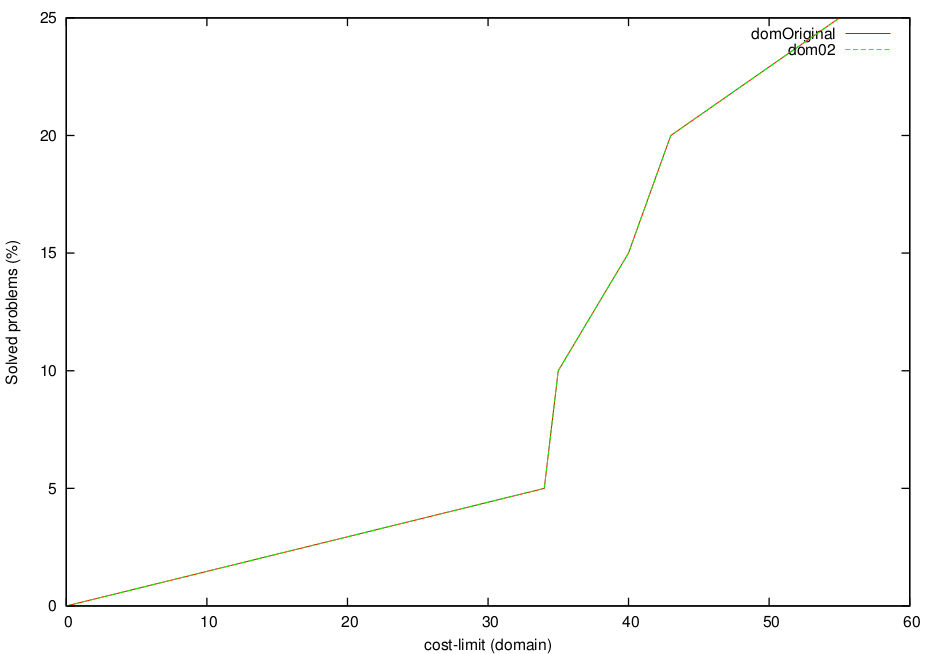
\includegraphics[width=12cm, height=8cm]{mff-or-02-cost}
        \caption{MFF-original-02-coste}
    \end{figure}
    
    \begin{figure}[H]
        \centering
        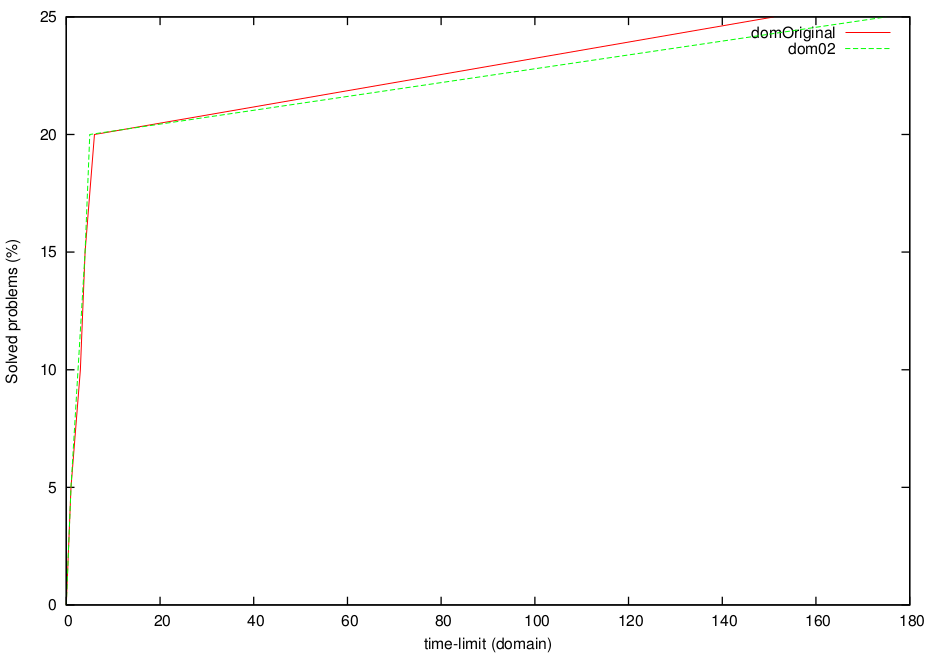
\includegraphics[width=12cm, height=8cm]{mff-or-02-time}
        \caption{MFF-original-02-tiempo}
    \end{figure}
    
    \begin{figure}[H]
        \centering
        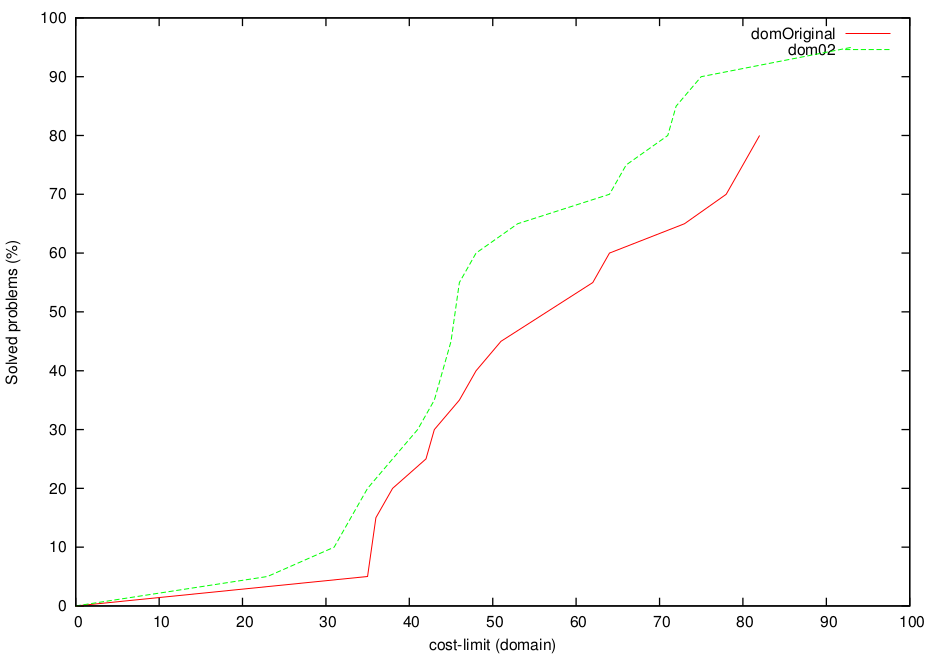
\includegraphics[width=12cm, height=8cm]{lpg-or-02-cost}
        \caption{LPG-original-02-coste}
    \end{figure}
    
    \begin{figure}[H]
        \centering
        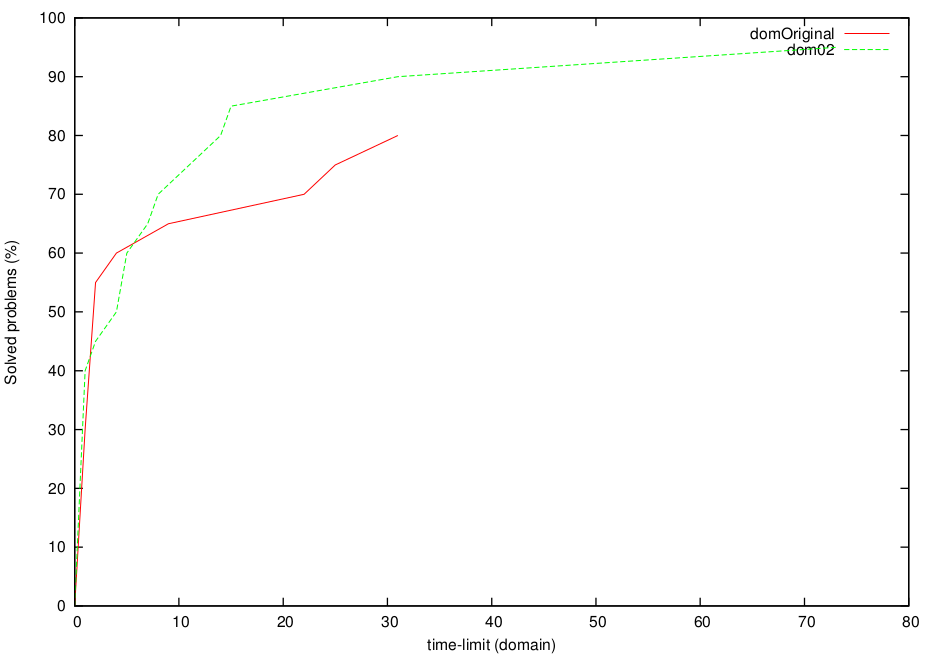
\includegraphics[width=12cm, height=8cm]{lpg-or-02-time}
        \caption{LPG-original-02-tiempo}
    \end{figure}
    
    \paragraph{}
    Como se puede ver en las figuras 8 y 9, esta versión reduce ligeramente el tiempo de búsqueda y esta mejora se va acrecentando a medida que aumenta el tamaño de los problemas. Esto es debido a que con el aumento del tamaño de los mismos, aumenta la probabilidad de que ocurra el caso particular en el que el segundo dominio provoca una reducción del tiempo de búsqueda. Respecto al coste, se puede ver en la figura 9 que es idéntico en ambos casos, puesto que realmente lo que se consigue con esta nueva versión es podar del árbol de búsqueda soluciones duplicadas (que podrían ser obtenidas mediante el otro operador de crear sándwiches con gluten), por lo que la solución final encontrada por ambas versiones es muy probable que acabe siendo la misma.
    
    \paragraph{}
    Las figuras 10 y 11 obtenidas con LPG-td son más difíciles de interpretar y no siguen el mismo patrón que en \textit{Metric-FF}. En estas, con la nueva versión sí se producen importantes modificaciones tanto en el tiempo consumido como en el coste de las soluciones obtenidas. Respecto al tiempo consumido, con la versión original se resuelven 3 problemas menos y los problemas resueltos requieren de más tiempo. Por otro lado, se puede ver en la figura 10 que el coste de resolución de estos problemas es también superior en la versión original.
    
    \subsubsection{Comparación del dominio09 y dominio11}
    \paragraph{}
    En estas versiones, se realiza exclusivamente la modificación de los predicados aumentando o disminuyendo su tamaño. En el caso de la versión 09, se aumenta dicho tamaño al juntar los predicados de \cool{allergic\_gluten} y \cool{not\_allergic\_gluten} con el predicado \cool{waiting}, ya que en ambas partes de los predicados originales se refiere a la misma variable \cool{child}. En la versión 11, se sustituye el predicado de negación \cool{not\_allergic\_gluten} por la negación del predicado \cool{allergic\_gluten} es decir, \cool{(not(allergic\_gluten))}.
    
    \begin{figure}[H]
        \centering
        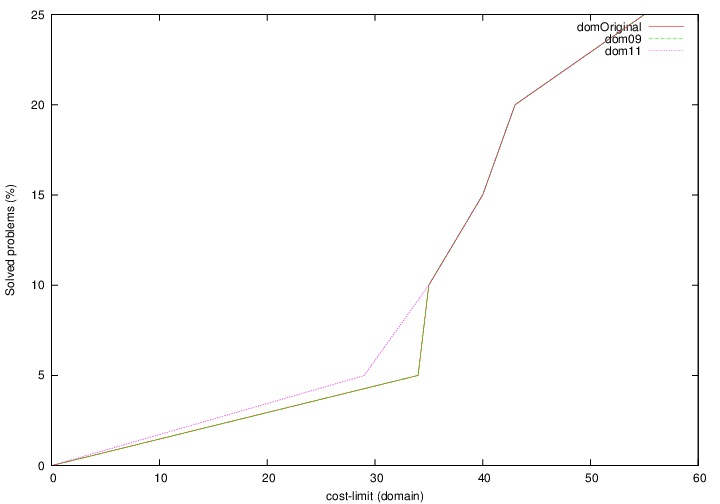
\includegraphics[width=12cm, height=8cm]{mff-or-09-11-cost}
        \caption{MFF-original-09-11-coste}
    \end{figure}
    
    \begin{figure}[H]
        \centering
        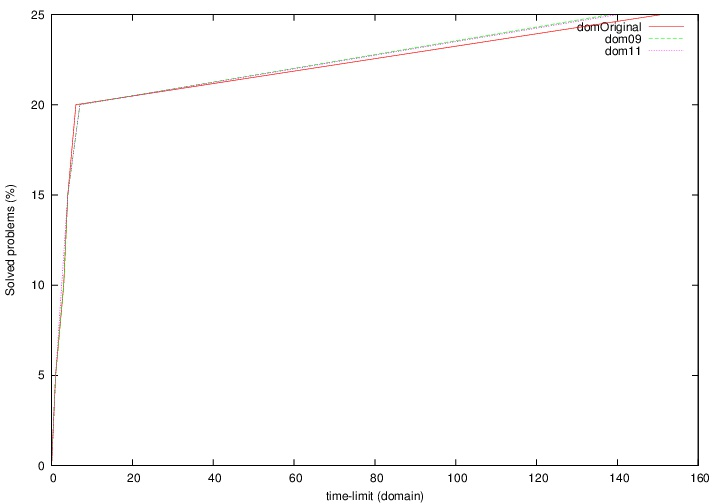
\includegraphics[width=12cm, height=8cm]{mff-or-09-11-time}
        \caption{MFF-original-09-11-tiempo}
    \end{figure}
    
    \begin{figure}[H]
        \centering
        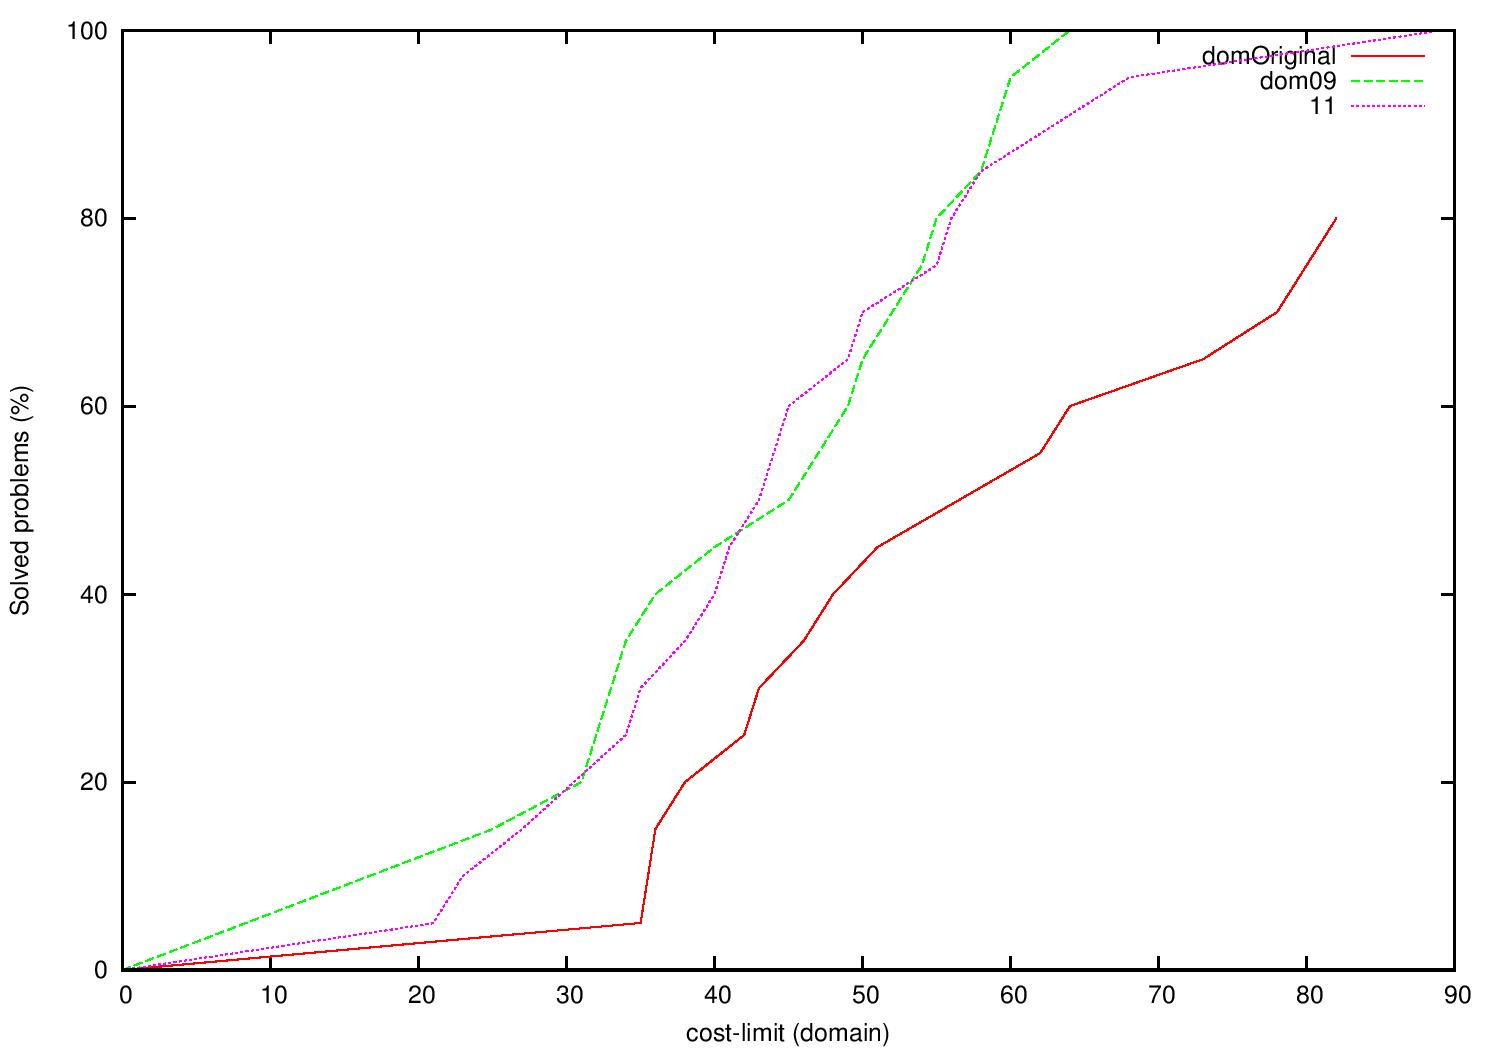
\includegraphics[width=12cm, height=8cm]{lpg-or-09-11-cost}
        \caption{LPG-original-09-11-coste}
    \end{figure}
    
    \begin{figure}[H]
        \centering
        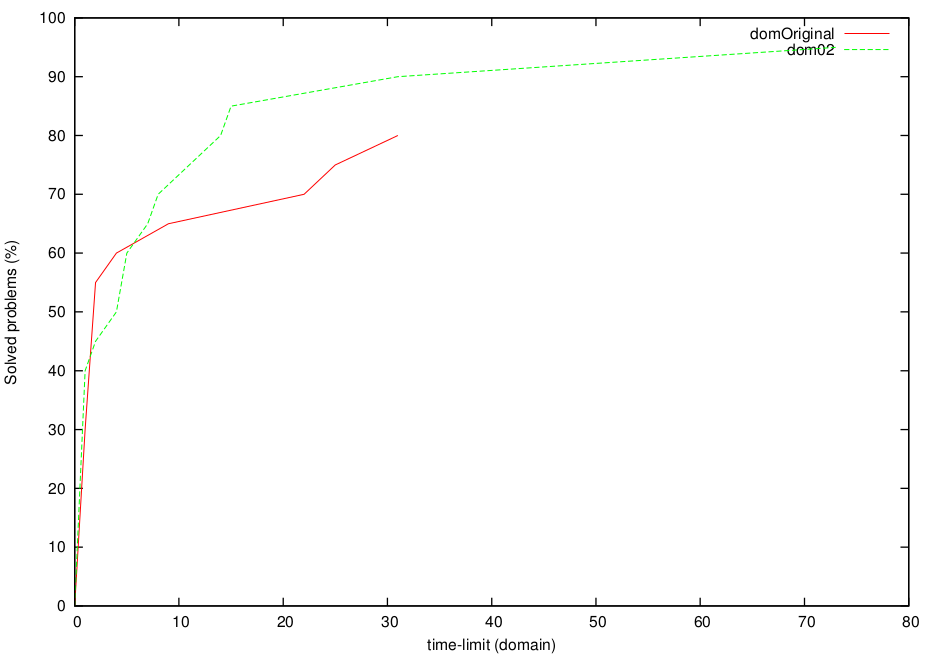
\includegraphics[width=12cm, height=8cm]{lpg-or-02-time}
        \caption{LPG-original-09-11-tiempo}
    \end{figure}
    
    \paragraph{}
    Respecto a los resultados obtenidos con MFF que se muestran en las figuras 12 y 13, con la versión 09 se obtienen soluciones con exactamente el mismo coste que en la versión original a diferencia de la versión 11, con la que se obtienen problemas con menor coste hasta llegar a problemas con una complejidad en la que convergen los costes de las tres versiones. Respecto a los problemas y el tiempo de resolución, todos convergen en la resolución de el 25\% de los problemas pero con una ligera reducción de tiempo de búsqueda en las dos versiones realizadas a mano, tal y como se puede observar en la figura 13. Al haberse realizado modificaciones pequeñas de los predicados, no se esperaban grandes cambios en la calidad y los tiempos de ejecución, por lo que era previsible que estos resultados fueran cercanos a los obtenidos con la versión original.
    
    \paragraph{}
    En relación a los resultados obtenidos con LPG-td que se muestran en las figuras 14 y 15, estos son mucho más impredecibles y difíciles de interpretar. Ambas versiones consiguen aumentar el porcentaje de problemas resueltos de en torno al 80\% al 100\%. Se puede apreciar en la figura 14 que el coste de dichas resoluciones es inferior que en el caso original y dependiendo del tramo es mayor o menor el coste entre ambas versiones. Finalmente, respecto al tiempo de ejecución, se puede apreciar en la figura 15 que los menores tiempos se obtienen con la versión 09, aunque con la versión 11 también se reducen los tiempos de ejecución respecto a la versión original.
    
    \subsubsection{Comparación de los dominios numéricos}
    \paragraph{}
    En esta sección, se van a comparar tanto los dominios numéricos realizados a mano como los dominios numéricos obtenidos obtenidos mediante software independiente de dominio de otros desarrolladores. Respecto a los dominios numéricos realizados a mano, la versión 05 corresponde a la versión numérica con proposiciones mientras que la versión 08 corresponde a la versión numérica con dígitos.
    
    \begin{figure}[H]
        \centering
        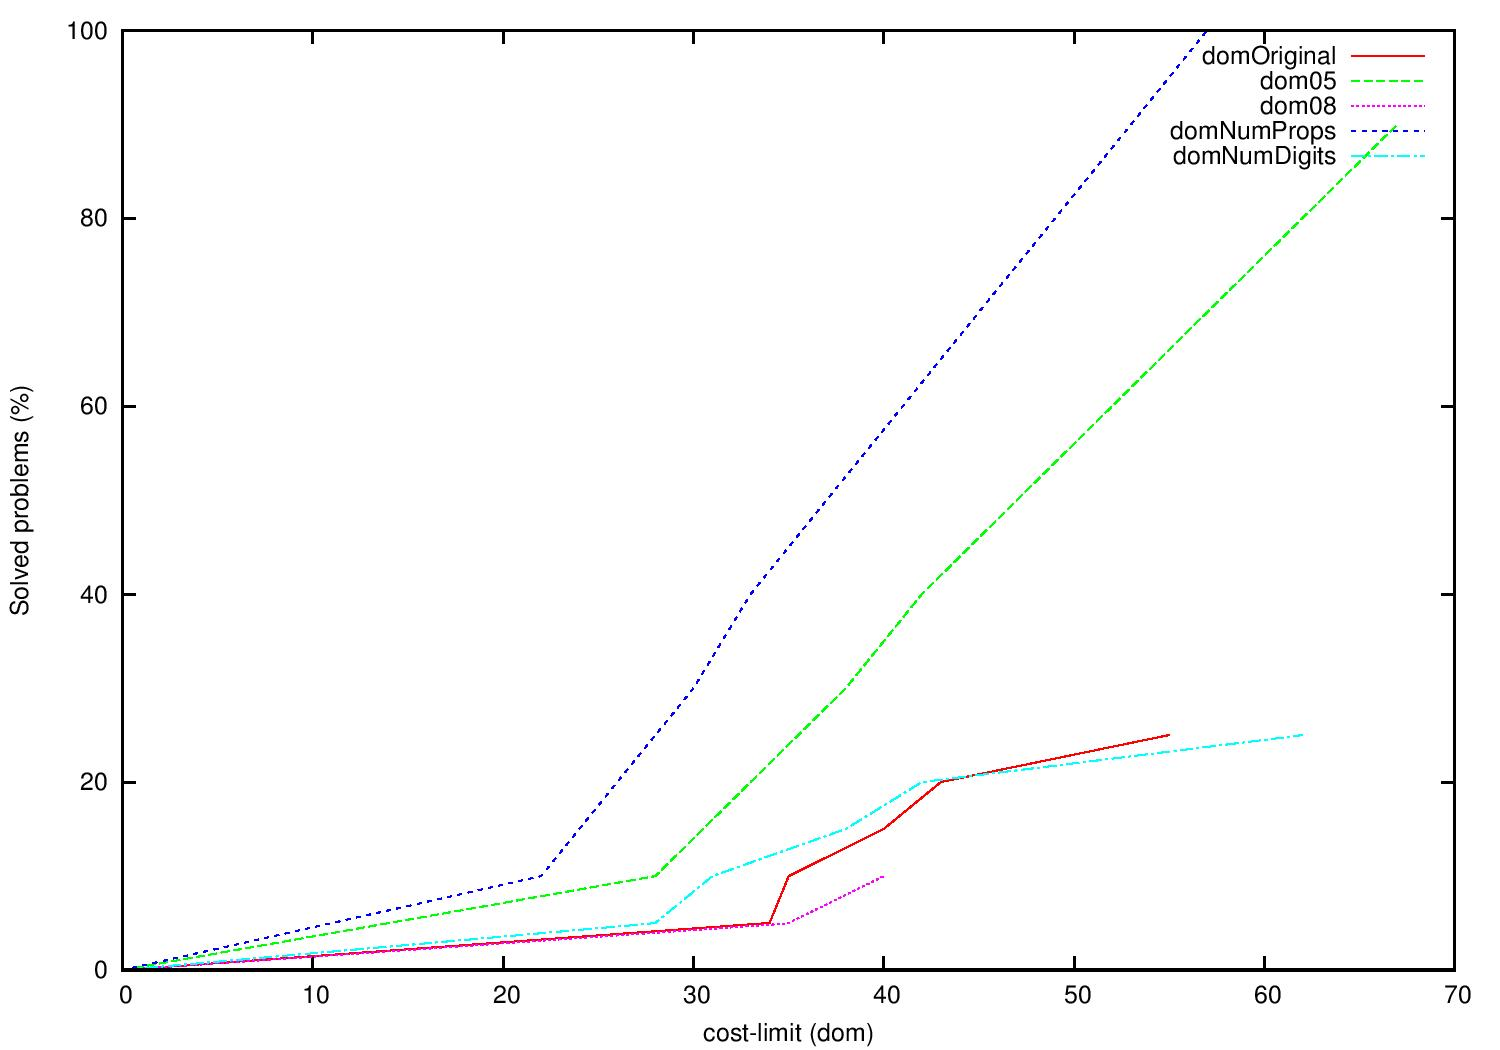
\includegraphics[width=12cm, height=8cm]{mff-or-05-08-prop-digit-cost}
        \caption{MFF-original-02-coste}
    \end{figure}
    
    \begin{figure}[H]
        \centering
        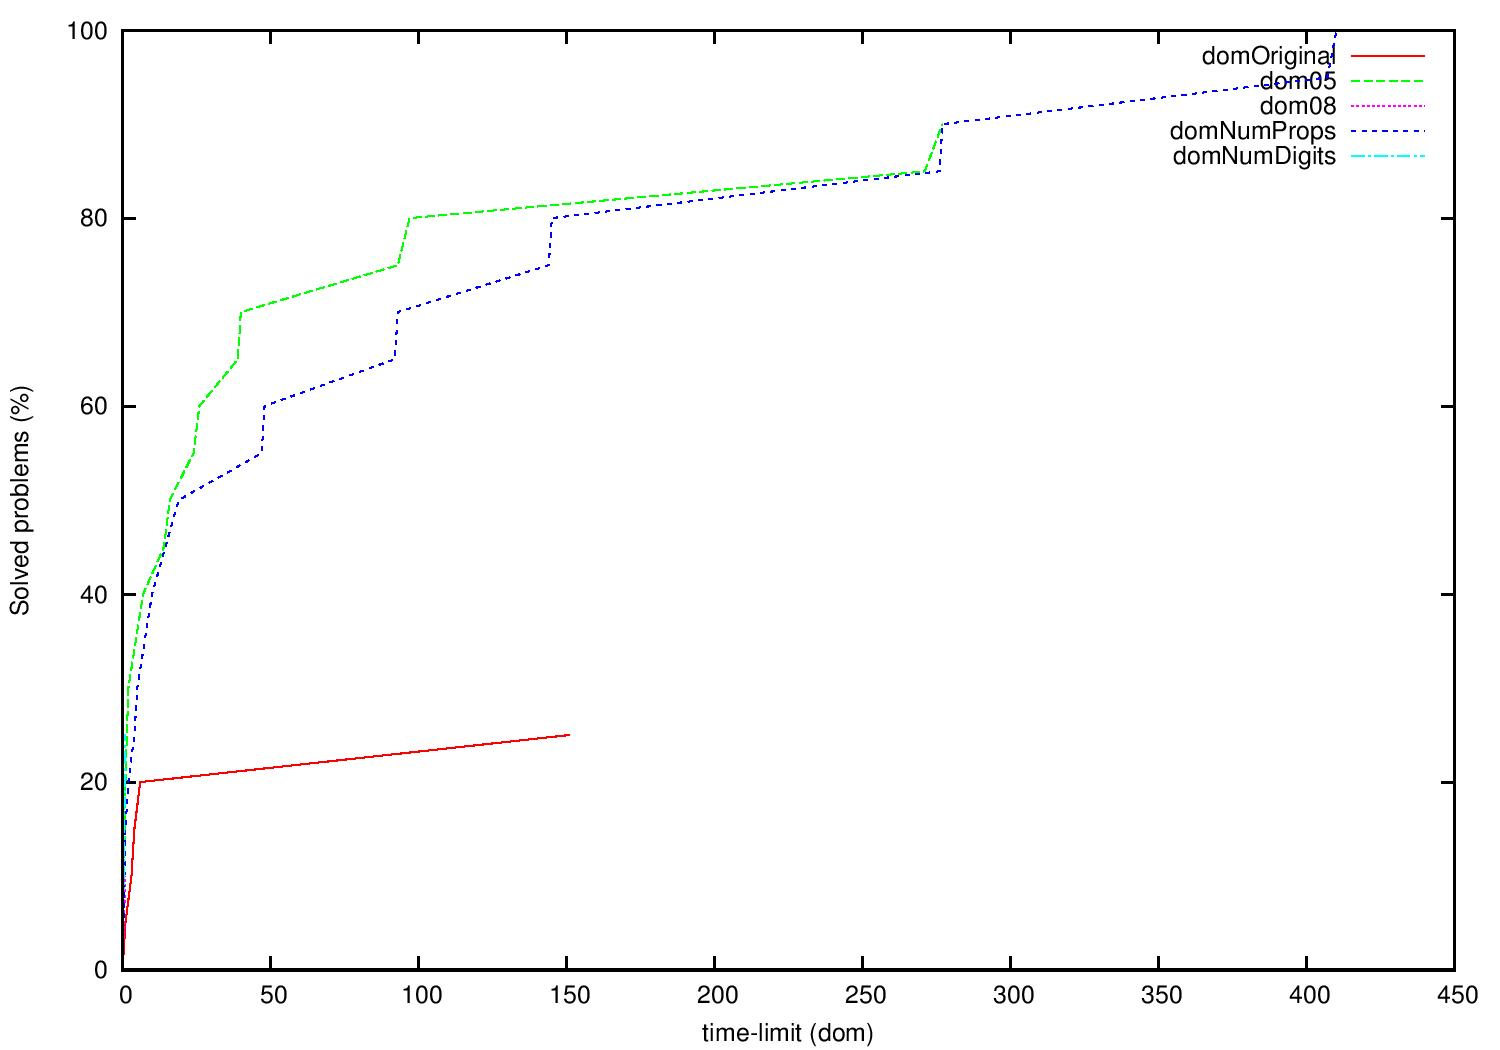
\includegraphics[width=12cm, height=8cm]{mff-or-05-08-prop-digit-time}
        \caption{MFF-original-02-tiempo}
    \end{figure}
    
    \begin{figure}[H]
        \centering
        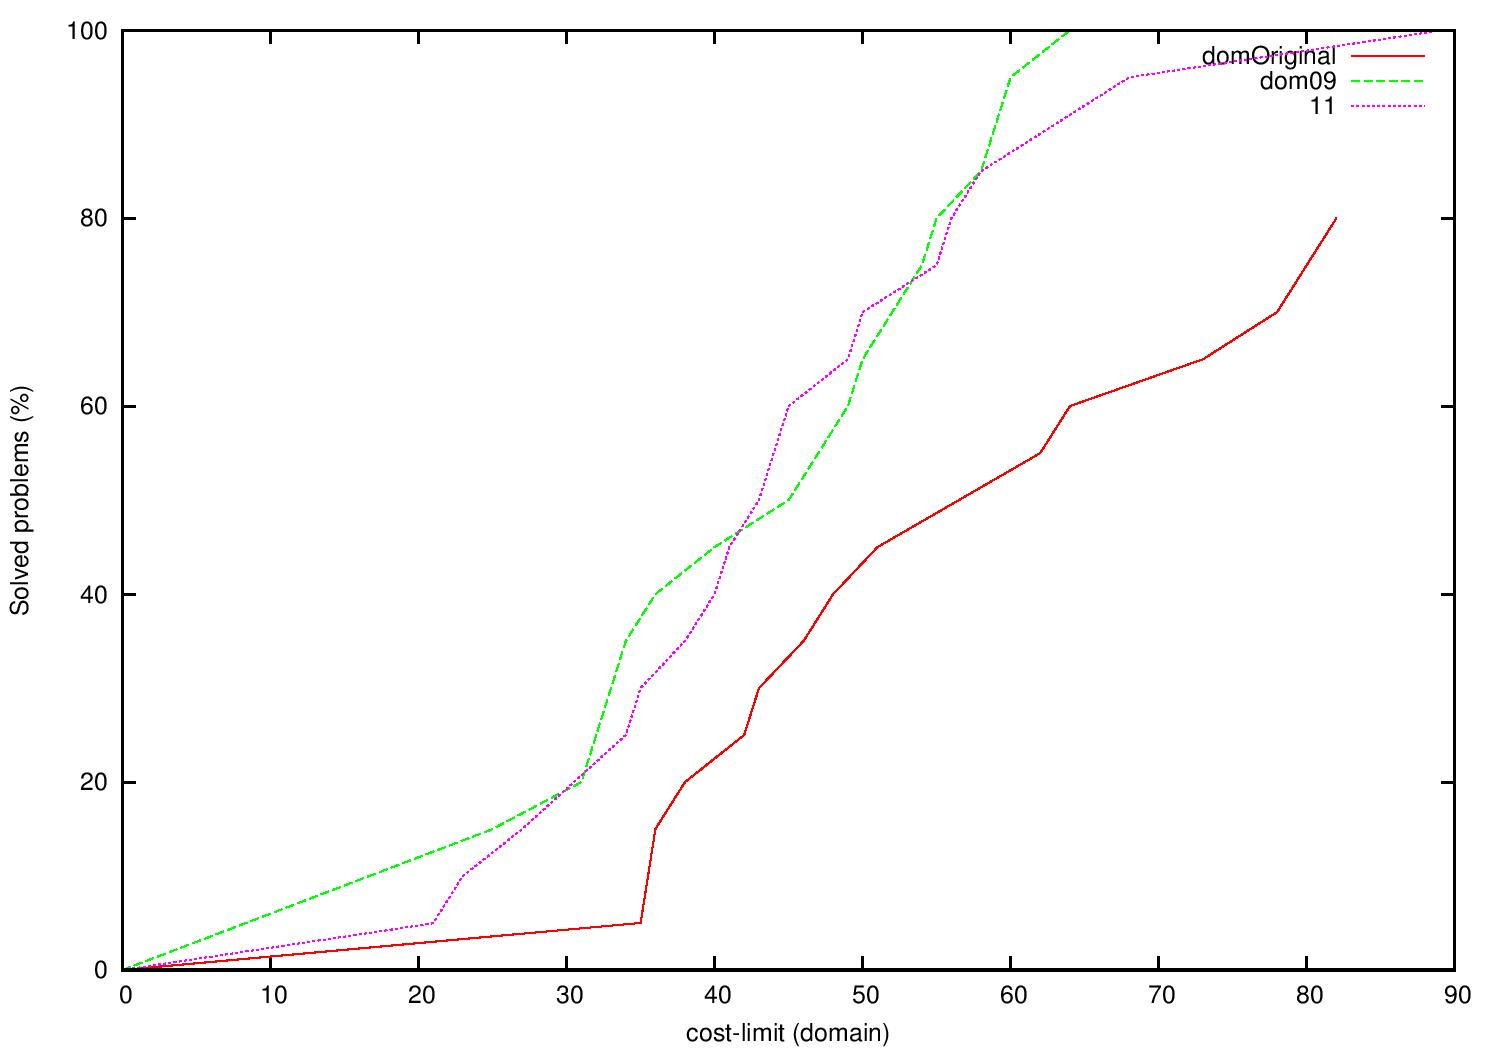
\includegraphics[width=12cm, height=8cm]{lpg-or-05-08-prop-digit-cost}
        \caption{LPG-original-02-coste}
    \end{figure}
    
    \begin{figure}[H]
        \centering
        \includegraphics[width=12cm, height=8cm]{lpg-or-05-08-prop-digit-time}
        \caption{LPG-original-02-tiempo}
    \end{figure}
    
    \begin{figure}[H]
        \centering
        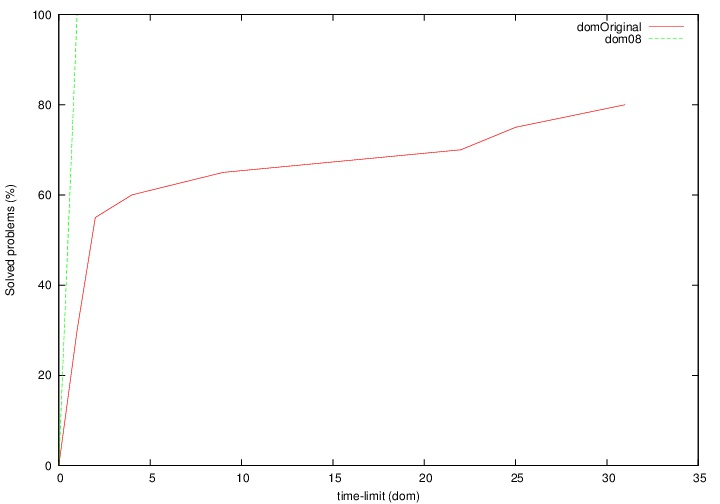
\includegraphics[width=12cm, height=8cm]{lpg-or-08-time}
        \caption{LPG-original-08-tiempo}
    \end{figure}
    
    \paragraph{}
    En la figura 17, prácticamente no se ve el resultado de la versión numérica con dígitos generada automáticamente. Esto se debe a que está superpuesta con el principio de la versión 05. Al quedarse la gráfica en un valor de resolución de problemas del 25\% de los problemas de entrada, queda patente que esta versión comparada con el resto de versiones no es la mejor de las soluciones. Sin embargo, este resultado coincide con el porcentaje de problemas resueltos por la versión original requiriendo por otro lado mucho menos tiempo. Por otro lado, supera en el número de problemas resueltos y en un coste similar a la versión 08, tal y como se ve en la figura 16. A su vez, el coste de las soluciones obtenidas con la versión numérica con dígitos es similar al coste de la versión original, variando la versión con mayor coste entre estas dos versiones entre los distintos problemas resueltos.
    
    \paragraph{}
    Los mejores resultados obtenidos con el planificador MFF se obtienen con las versiones numérica con palabras y la versión 05, resolviendo más problemas y con menor coste con la versión automática numérica con palabras, pero requiriendo más tiempo que en la versión 05.
    
    \paragraph{}
    Respecto a la versión numérica con proposiciones generada automáticamente y la versión realizada manualmente (versión 05), se puede observar en los resultados de las figuras 16 y 17 que con el planificador \textit{MFF} que en términos generales la versión generada automáticamente obtiene mejores resultados. En este caso, es difícil intentar desgranar los motivos subyacentes puesto que la versión automática genera bastantes nuevos predicados que son complicados de interpretar y la versión final que se genera tiene una estructura totalmente distinta de la que aparece en la versión manual.
    
    \paragraph{}
    Por otro lado, en las versiones numéricas con dígitos, los resultados son muy similares puesto que los problemas de entrada tienen una representación común y en lo único que varían los dominios es en uno de los operadores (toda la información referente a este cambio se puede encontrar en la sección de solución propuesta). En los resultados, se puede ver en las figuras 16 y 17 que con la versión automática se resuelven más problemas en la versión automática, teniendo esta un coste mayor pero obteniendo estas soluciones en un tiempo similar.
    
    \paragraph{}
    Respecto a los resultados de \textit{LPG-td} que aparecen en las figuras 18, 19 y 20, la versión automática numérica con proposiciones vuelve a resolver la totalidad de los problemas, al igual que también lo hace la versión numérica con proposiciones generada manualmente (la versión 08). Esto quiere decir que sin lugar a dudas la transformación automática para generar un dominio con proposiciones es beneficiosa para ambos planificadores.
    
    \paragraph{}
    Respecto a los costes para resolver los problemas, se puede ver en la figura 18 que los menores costes se obtienen con la versión 08, que en su tramo de problemas iniciales se superpone con el coste de la versión original. En lo que concierne a los tiempos, se puede ver en la figura 19 que la versión más rápida en la gráfica en la que aparecen representados los tiempos de las 5 versiones pudiera parecer que es la versión original. Sin embargo, en realidad la versión más rápida es la versión 08, como se puede ver en la figura 20 que se ha añadido incluyendo exclusivamente las gráficas de tiempo de la versión que aparenta ser la más rápida (la original) y la que realmente es significativamente más rápida (la versión 08). En la figura 19 no se puede ver nítidamente el tiempo de la versión 08 debido a que como la diferencia de tiempos es tan grande respecto al resto de versiones, este tiempo está tan próximo a cero que es muy complicado ver estos tiempos en esta gráfica.
    
    \subsubsection{Comparación del dominio12}
    
    \paragraph{}
    Este es un dominio por etapas en el que se ha intentado obtener la mejor versión posible respecto a tanto el tiempo de búsqueda como al coste de obtención de las soluciones. Para crear este dominio, han sido necesarios añadir nuevos operadores, que como se comentará a continuación, han aumentado el coste de las soluciones.
    
    \paragraph{}
    Como este es el dominio que ha sido diseñado específicamente para ser la mejor versión de todas, no solo se va a comparar el resultado con la versión original, sino que se va a comparar el coste de la solución de los problemas con el coste óptimo de la solución de cada uno de los problemas.
    
    \paragraph{}
    La solución óptima para cualquier problema de \textit{Childsnack} (cuya lógica es en la que se ha basado esta versión del dominio) consiste en aprovechar que las bandejas tienen una capacidad infinita para únicamente utilizar una bandeja para la resolución del problema, puesto que utilizar más bandejas implica realizar al menos el mismo número de desplazamientos que con una única bandeja, por lo que para simplificar el árbol de búsqueda se va a acotar las soluciones obtenidas a aquellas en las que únicamente se hace uso de una bandeja. A su vez, para cada niño que haya que servir hará falta: realizar un sándwich, cargarlo en la bandeja y servirlo. Considerando que la bandeja está en la cocina y todos los niños están en la misma localización, como mínimo será necesario el desplazamiento desde la cocina a la localización en la que estén todos los niños que haya que servir (salvo en el caso de que todos los niños estén en la cocina, en cuyo caso no hace falta desplazamiento). Por otra, parte, en el peor de los casos, ninguna de las bandejas estará colocada inicialmente en la cocina (lo que supondrá el coste de una acción para desplazarla a la cocina para poder cargar los śandwiches) y cada niño estará en una posición distinta, por lo que a las acciones anteriores será necesario añadir una acción de desplazamiento de la bandeja por cada niño a servir. Por tanto, el número de pasos óptimo o coste para resolver cualquien problema de Childsnack queda definido por la siguiente fórmula: \\
    
    $#niños\times3 \leq Coste \´optimo \leq niños\times4+1$
    
    \paragraph{}
    A partir de esta fórmula genérica, se puede acotar hasta saber directamente el coste exacto de la solución óptima si se cuenta con la información referente al número de localizaciones distintas en las que están los niños sin contar aquellos que puedan estar en la cocina ($a$) y si existe alguna bandeja en la cocina ($b$). Así, el coste exacto de la solución óptima para cualquier problema de Childsnack en su versión original es:
    
    $Coste \´optimo = #niños\times3 + a + b$
    
    \paragraph{}
    Con esta fórmula se obtienen los resultados de los costes óptimos para cada problema de entrada que se encuentra en la tabla 2. Por poner un ejemplo de cómo se obtienen este valor así como un plan que demuestre que existe una solución con el coste óptimo obtenido con esta fórmula, se va a obtener el coste óptimo y un plan óptimo para el problema 01-2 de la versión original.
    
    \paragraph{}
    En el problema 01-2, los datos que observamos que son necesarios meter como entrada para la obtención del coste óptimo son los siguientes:
    \begin{itemize}
        \item #niños = 6
        \item a = 3 (los niños que hace falta servir están en las localizaciones \cool{table1}, \cool{table2} y \textit{table3}.
        \item b = 0 (las bandejas portátiles \cool{tray1} y \cool{tray2} están en la cocina).
    \end{itemize}
    
    Por tanto, se obtendría que el coste óptimo para el problema 01-2 de la versión original es de $coste \´optimo = 6*3+3+0=21$.
    
    \paragraph{}
    Una posible solución con este coste para este problema sería la siguiente: \\
    
    \noindent{}\cool{
    0: MAKE\_SANDWICH\_NO\_GLUTEN  SANDW1 BREAD2  CONTENT3 \\
    1: MAKE\_SANDWICH\_NO\_GLUTEN  SANDW2 BREAD5  CONTENT6 \\
    2: MAKE\_SANDWICH              SANDW3 BREAD1  CONTENT1 \\
    3: MAKE\_SANDWICH              SANDW4 BREAD3  CONTENT2 \\
    4: MAKE\_SANDWICH              SANDW5 BREAD4  CONTENT4 \\
    5: MAKE\_SANDWICH              SANDW6 BREAD6  CONTENT5 \\
    6: PUT\_ON\_TRAY               SANDW1 TRAY1 \\
    7: PUT\_ON\_TRAY               SANDW2 TRAY1 \\
    8: PUT\_ON\_TRAY               SANDW3 TRAY1 \\
    9: PUT\_ON\_TRAY               SANDW4 TRAY1 \\
    10:PUT\_ON\_TRAY               SANDW5 TRAY1 \\
    11:PUT\_ON\_TRAY               SANDW6 TRAY1 \\
    12:MOVE\_TRAY                  TRAY1  KITCHEN TABLE1 \\
    13:SERVE\_SANDWICH\_NO\_GLUTEN SANDW1 CHILD5  TRAY1  TABLE1 \\
    14:SERVE\_SANDWICH             SANDW3 CHILD2  TRAY1  TABLE1 \\
    15:SERVE\_SANDWICH             SANDW4 CHILD6  TRAY1  TABLE1 \\
    16:MOVE\_TRAY                  TRAY1  TABLE1  TABLE2 \\
    17:SERVE\_SANDWICH\_NO\_GLUTEN SANDW2 CHILD1  TRAY1  TABLE2 \\
    18:SERVE\_SANDWICH             SANDW5 CHILD4  TRAY1  TABLE2 \\
    19:MOVE\_TRAY                  TRAY1  TABLE2  TABLE3 \\
    20:SERVE\_SANDWICH             SANDW6 CHILD3  TRAY1  TABLE3} \\
    
    \paragraph{}
    Por último, si se observa detenidamente esta solución, se podrá ver que no hay ningún conjunto de acciones que se pueda realizar en un menor número de pasos. Todos los sándwiches tienen que hacerse, por lo que hasta el paso 5 no hay ninguna reducción de costes posibles. Todos los sándwiches tienen que ser cargados en alguna bandeja, porque sólo se pueden servir sándwiches cargados, por lo que los pasos 6-11 no pueden ser simplificados. Es necesario una acción por cada sándwich que se sirva y no se puede servir un sándwich si no se encuentra la bandeja que contiene ese sándwich en la misma localización que el niño al que se va a servir, por lo que tampoco existe ninguna manera de reducir el número de acciones en el tramo 13-20. Por tanto, con este ejemplo empírico queda patente que la fórmula utilizada es correcta.
    
    
    \begin{figure}[H]
        \centering
        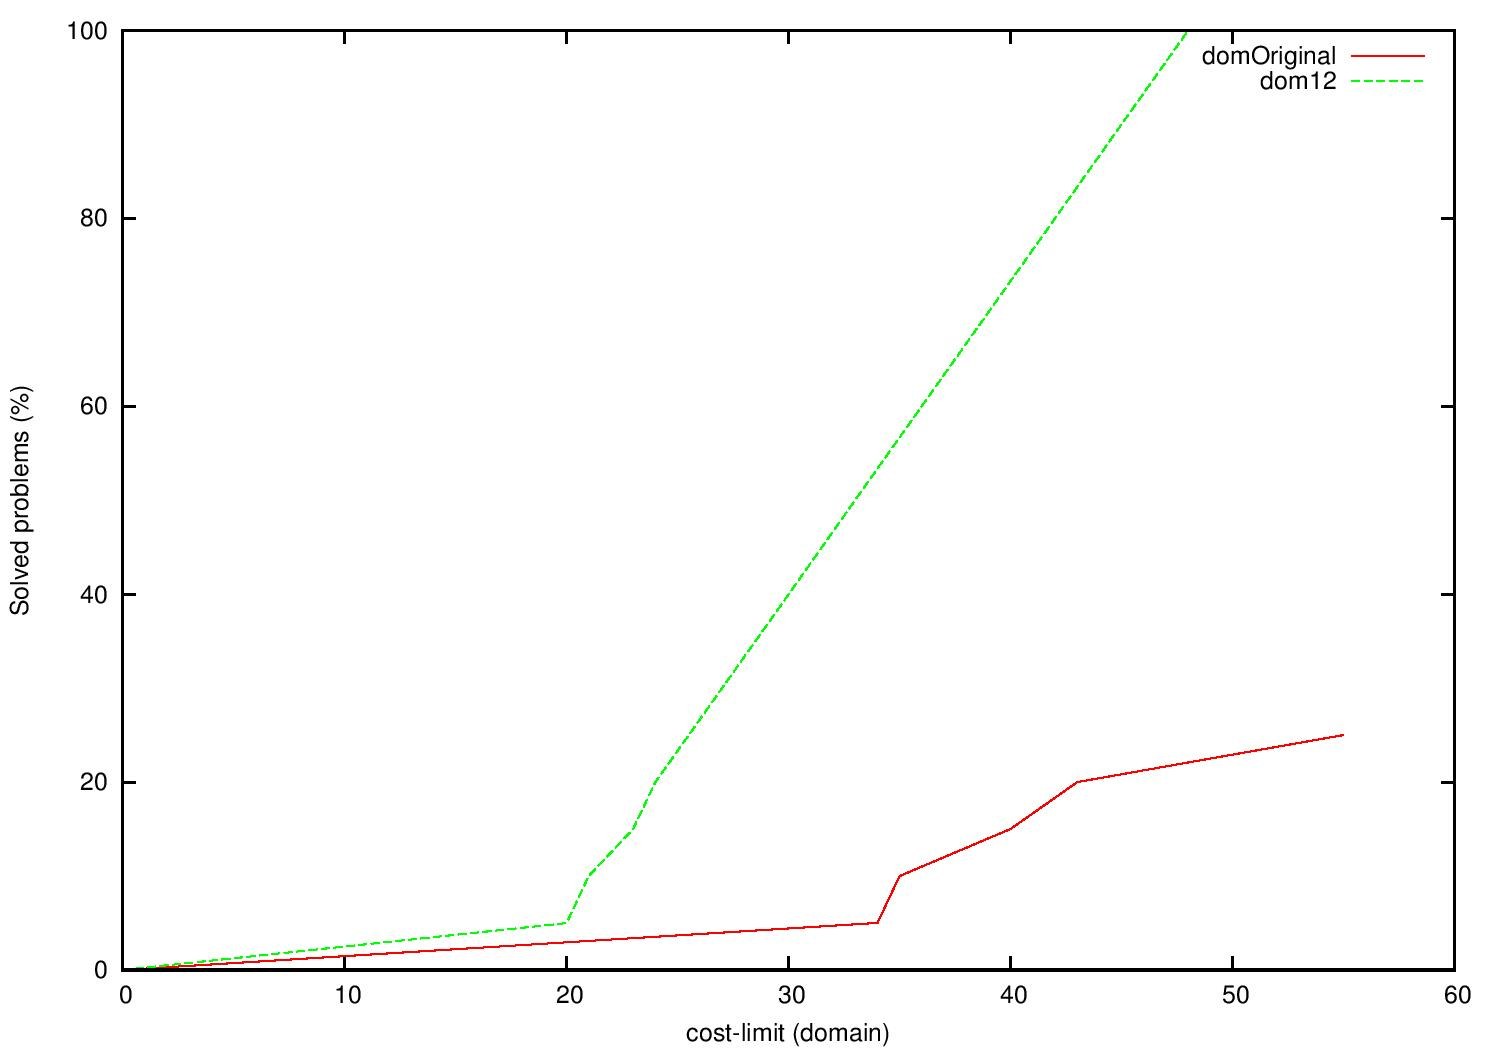
\includegraphics[width=12cm, height=8cm]{mff-or-12-cost}
        \caption{MFF-original-12-coste}
    \end{figure}
    
    \begin{figure}[H]
        \centering
        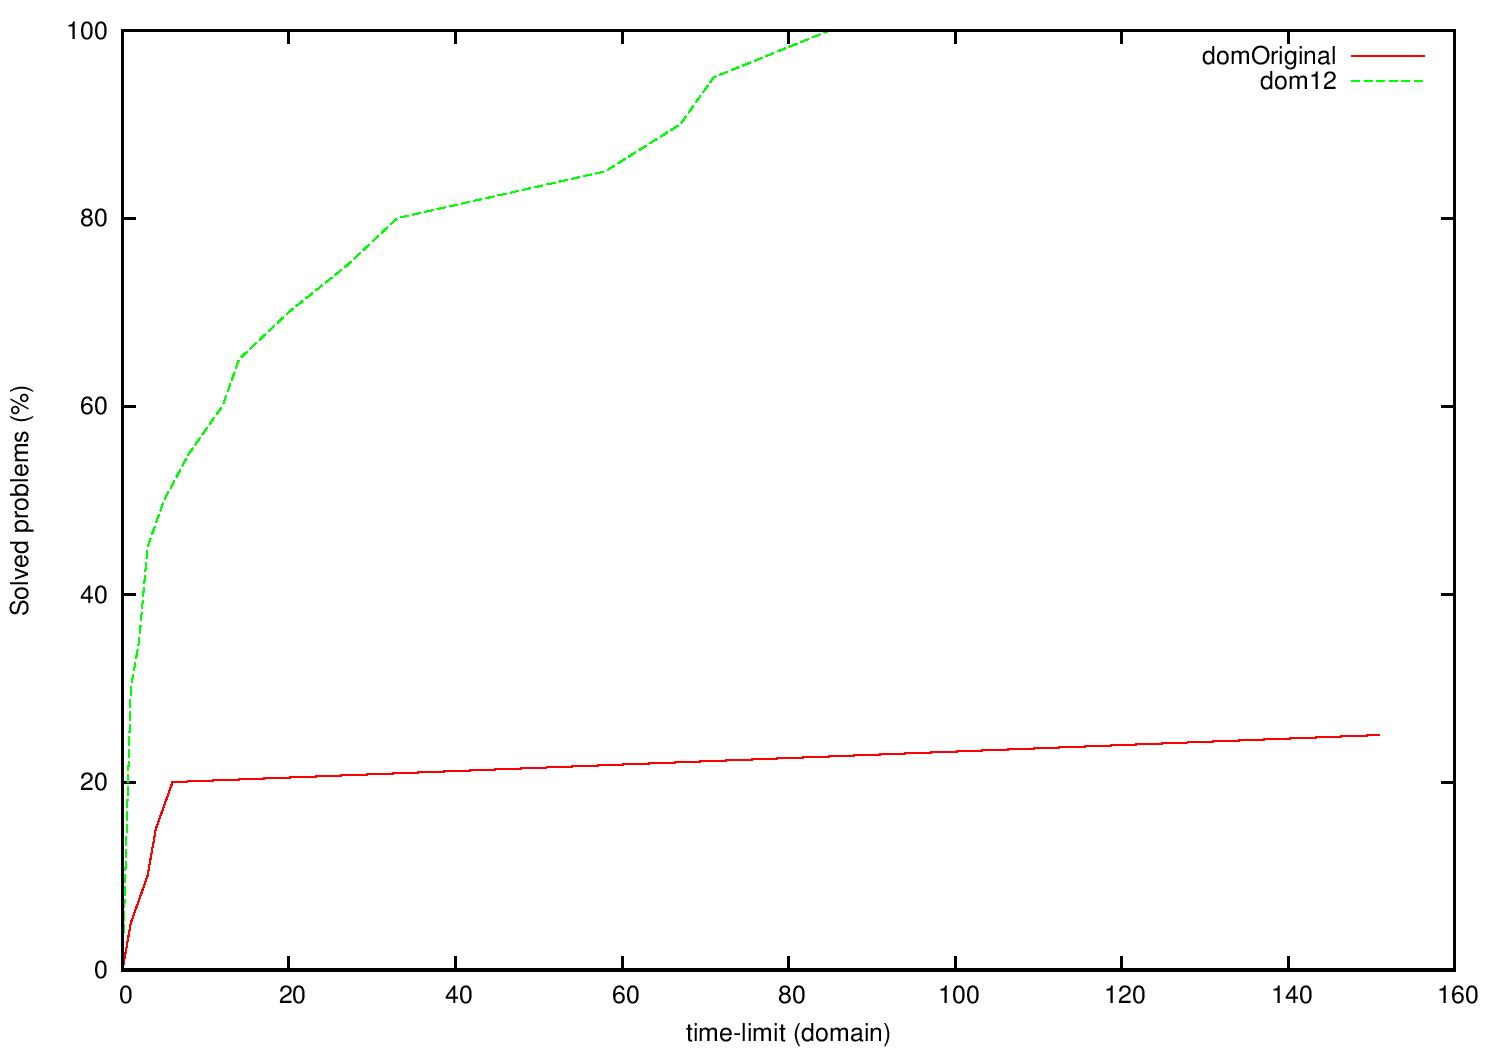
\includegraphics[width=12cm, height=8cm]{mff-or-12-time}
        \caption{MFF-original-12-tiempo}
    \end{figure}
    
    \begin{figure}[H]
        \centering
        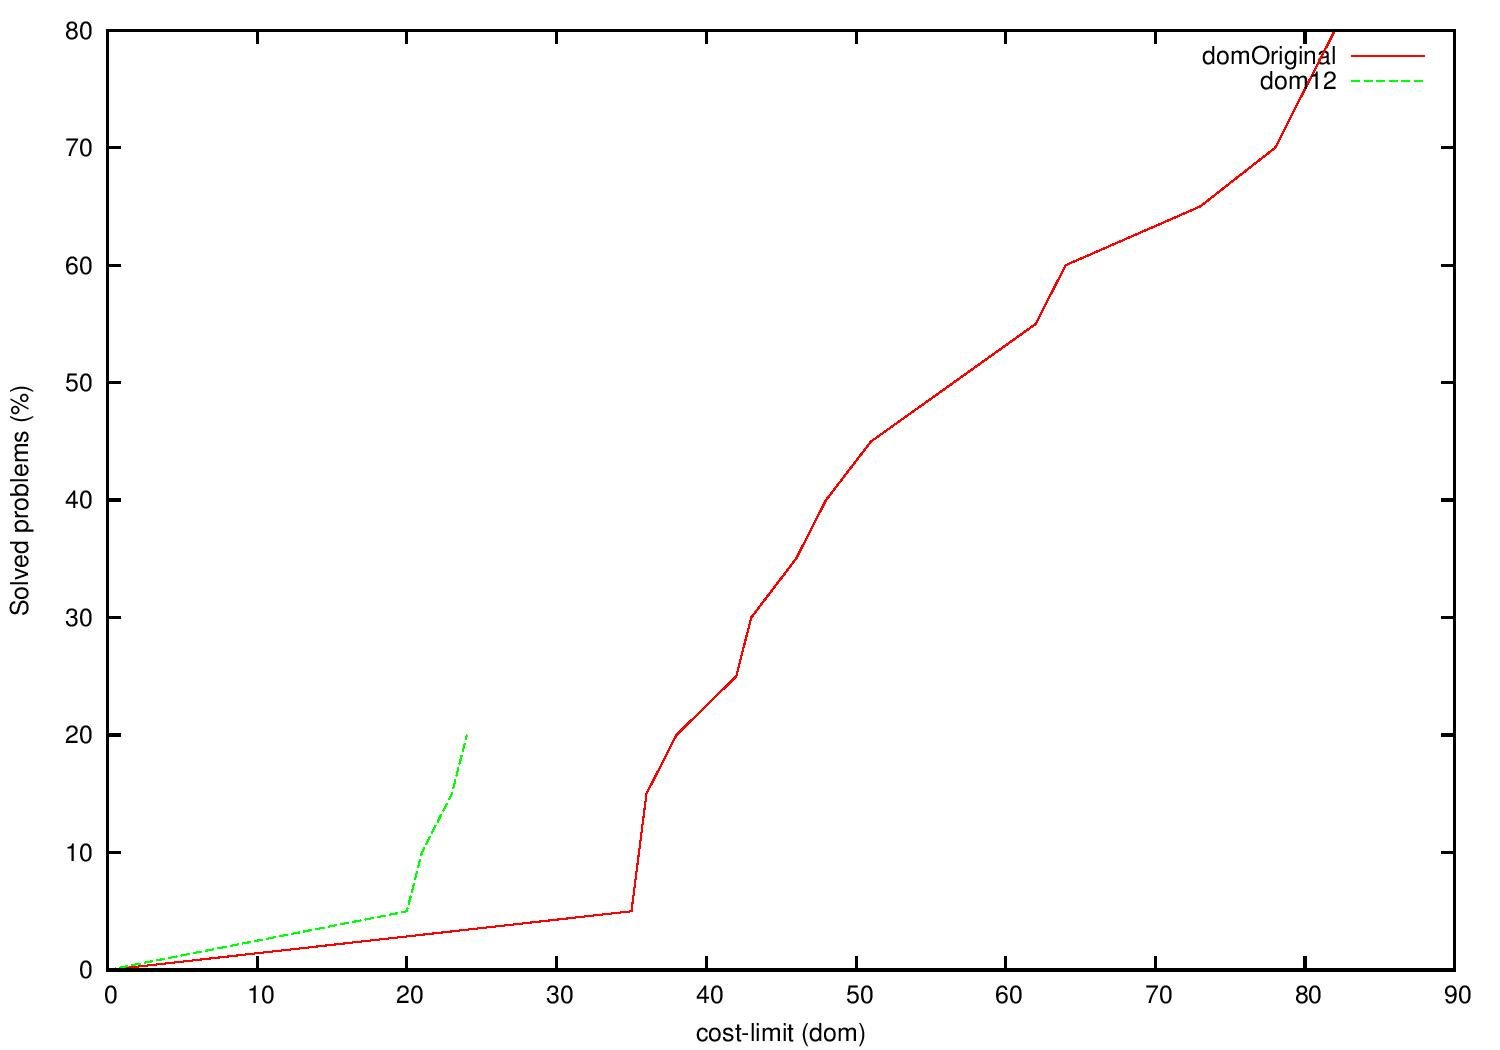
\includegraphics[width=12cm, height=8cm]{lpg-or-12-cost}
        \caption{LPG-original-12-coste}
    \end{figure}
    
    \begin{figure}[H]
        \centering
        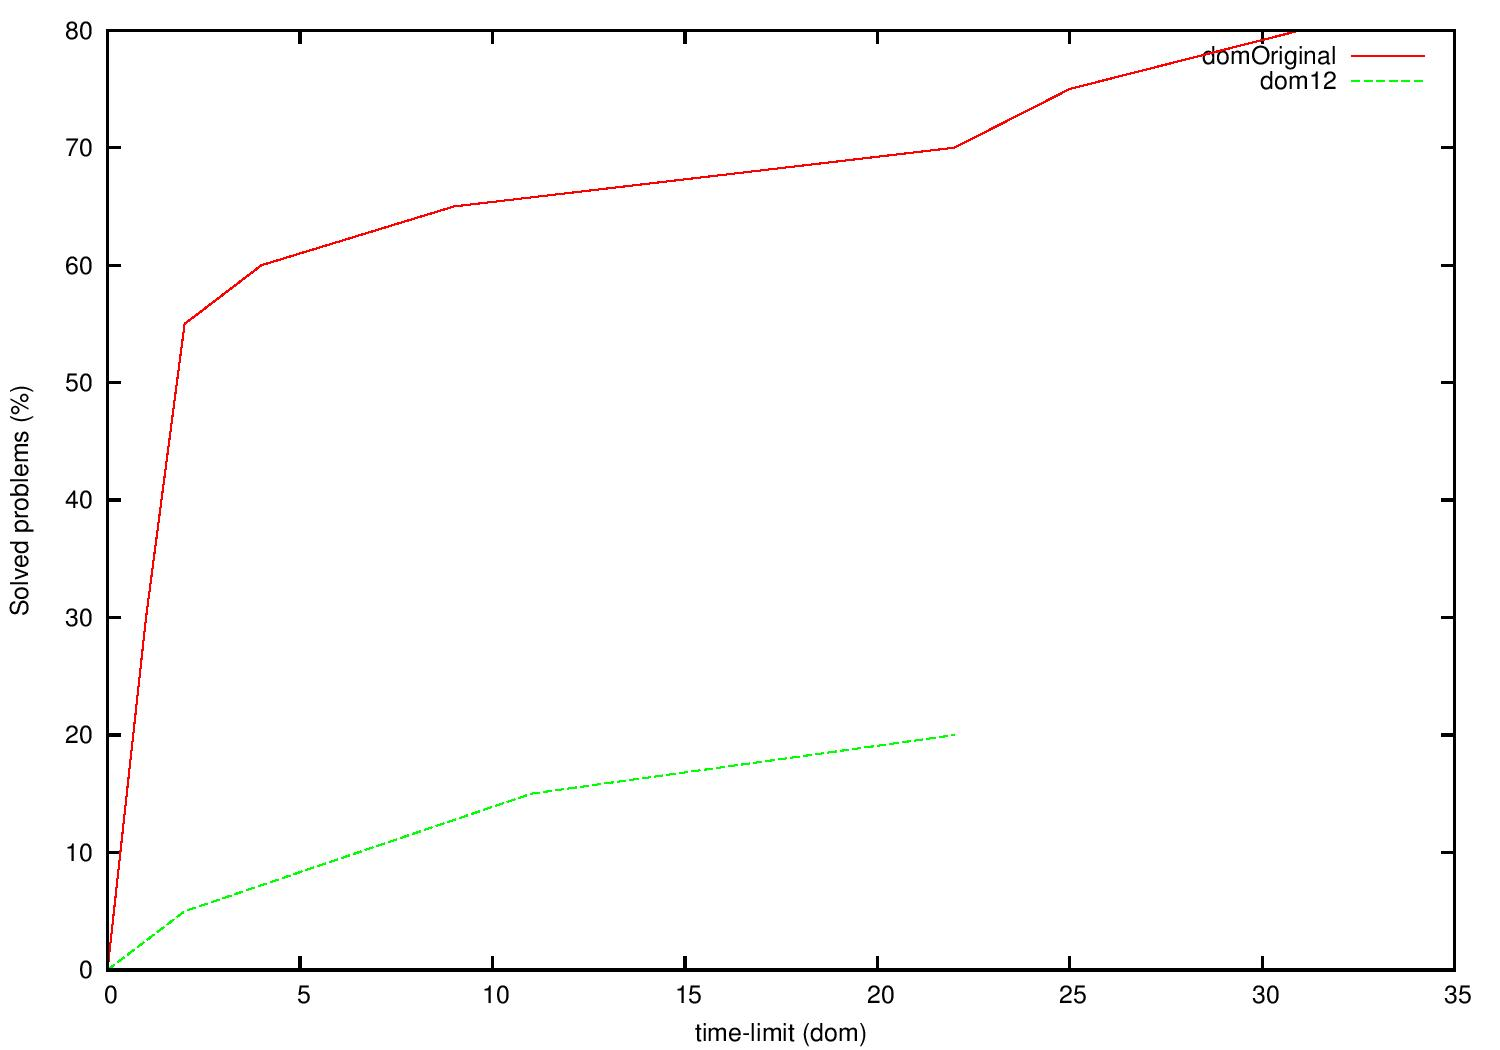
\includegraphics[width=12cm, height=8cm]{lpg-or-12-time}
        \caption{LPG-original-12-tiempo}
    \end{figure}
    
    \begin{table}[H]
    \centering
    \caption{Coste óptimo y coste de MFF}
    \label{my-label}
    \begin{tabular}{|c|c|c|}
    \hline
    \textbf{Problema} & \textbf{Coste óptimo} & \textbf{Coste MFF} \\ \hline
    01-2              & 21                    & \textbf{21}        \\ \hline
    01                & 20                    & \textbf{20}        \\ \hline
    02-2              & 24                    & \textbf{24}        \\ \hline
    02                & 22                    & 23                 \\ \hline
    03-2              & 27                    & \textbf{27}        \\ \hline
    03                & 27                    & \textbf{27}        \\ \hline
    04-2              & 30                    & \textbf{30}        \\ \hline
    04                & 30                    & \textbf{30}        \\ \hline
    05-2              & 33                    & \textbf{33}        \\ \hline
    05                & 33                    & \textbf{33}        \\ \hline
    06-2              & 36                    & \textbf{36}        \\ \hline
    06                & 36                    & \textbf{36}        \\ \hline
    07-2              & 39                    & \textbf{39}        \\ \hline
    07                & 39                    & \textbf{39}        \\ \hline
    08-2              & 39                    & 42                 \\ \hline
    08                & 39                    & 42                 \\ \hline
    09-2              & 45                    & \textbf{45}        \\ \hline
    09                & 45                    & \textbf{45}        \\ \hline
    10-2              & 48                    & \textbf{48}        \\ \hline
    10                & 48                    & \textbf{48}        \\ \hline
    \end{tabular}
    \end{table}
    
    \paragraph{}
    Como se puede ver en las figuras 21, 22, 23 y 24, vuelve a haber una gran diferencia entre las gráficas obtenidas con \textit{MFF} y con \textit{LPG-td}. En el caso de las figuras 21 y 22, se puede ver que esta modificación mejora muy significativamente tanto los tiempos de búsqueda como la calidad de las soluciones encontradas, hasta el punto de que como se puede observar en la tabla superior, en 17 de los 20 problemas originales el coste de la solución obtenida es el mismo que el menor que se podría obtener en cualquier versión que se hiciese de este problema, lo que convierte a esta versión en la mejor de todas las creadas.
    
    \paragraph{}
    Por contra, se puede observar en las figuras 23 y 24 que los resultados obtenidos utilizando el planificador \textit{LPG-td} son bastante peores que los obtenidos por la versión original en coste, tiempo de resolución y porcentaje de problemas resueltos. Una vez más, sería interesante poder analizar con mayor profundidad los motivos por los que se han obtenido estos resultados con el planificador \textit{LPG-td}, pero al no haber sido capaz de entender bien el funcionamiento de este planificador, no se puede explicar mejor los resultados que se han obtenido tras ejecutar este planificador
    
    \subsubsection{Comparaciones globales}
    \paragraph{}
    En esta sección, se va a incluir una comparativa de los resultados referentes a los tiempos y los costes de resolución de cada uno de los problemas para cada planificador por cada una de las versiones del dominio. De esta manera, se permitirá tener una visión más global de los resultados obtenidos. Las fórmulas que se utilizarán para esta comparativa son las mismas que la que se utilizan en las competiciones de la \textit{IPC} y son las siguientes: \\
    
    $puntuación_a(tiempo) = 
    \begin{cases}
        0      & \quad \text{si } a.E = -1\\
        \frac{1}{1 + log_{10}(\frac{a.D}{a.F})}  & \quad \text{si } a.E \neq -1 \\
    \end{cases}\\ \\ \\
     puntuación_a(calidad) = 
    \begin{cases}
        0      & \quad \text{si } a.E = -1\\
        \frac{1}{1 + log_{10}(\frac{a.E}{a.G})}  & \quad \text{si } a.E \neq -1 \\
    \end{cases}\\
    \text{
    Donde $a$ se define como la siguiente tupla:} \\
    a = (A, B, C, D, E, F, G) \\
    A = \text{problema actual.} \\
    B = \text{planificador utilizado.} \\
    C = \text{tiempo límite de la planificación.} \\ 
    D = \text{tiempo de búsqueda de la solución.} \\
    E = \text{coste de la solución (-1 si no ha sido resuelto).} \\
    F = \text{mejor tiempo de resolución del problema } A \text{ entre todas las versiones del problema.} \\
    G = \text{menor coste de resolución del problema } A \text{ entre todas las versiones del problema.} \\$
    
    \paragraph{}
    Aplicando esta fórmula para cada uno de los planificadores, obtenemos las tablas 3, 4, 5, 6 y 7 que observamos a continuación.
    
    \pagebreak
    
    \begin{landscape}
    \begin{table}[]
    \centering
    \caption{MFF tiempos \textit{IPC}}
    \label{my-label}
    \begin{tabular}{|c|c|c|c|c|c|c|c|c|c|c|c|}
    \hline
    \textbf{problema / versión} & \textbf{original} & \textbf{01}    & \textbf{02}    & \textbf{03}    & \textbf{05}    & \textbf{08}  & \textbf{09}    & \textbf{11}    & \textbf{12}    & \textbf{numProps} & \textbf{numDigits} \\ \hline
    \textbf{p01-2}  &  0,677  &  1      &  0,624  &  1      &  1      &  0      &  0,624  &  0,624  &  1      &  1      &  1     \\ \hline
    \textbf{p01}    &  0,677  &  1      &  0,624  &  0      &  1      &  0      &  0,624  &  0,624  &  1      &  1      &  0     \\ \hline
    \textbf{p02-2}  &  0,624  &  1      &  0,624  &  0,235  &  1      &  0      &  0,677  &  0,624  &  1      &  1      &  0     \\ \hline
    \textbf{p02}    &  0,315  &  1      &  0,308  &  0      &  1      &  0,235  &  0,318  &  0,318  &  1      &  1      &  0,235 \\ \hline
    \textbf{p03-2}  &  0      &  1      &  0      &  0      &  1      &  0      &  0      &  0      &  1      &  0,769  &  0     \\ \hline
    \textbf{p03}    &  0,235  &  1      &  0,235  &  0      &  0,769  &  0,235  &  0,235  &  0,235  &  1      &  0,589  &  0,235 \\ \hline
    \textbf{p04-2}  &  0      &  1      &  0      &  0      &  0,769  &  0      &  0      &  0      &  1      &  0,624  &  1     \\ \hline
    \textbf{p04}    &  0      &  1      &  0      &  0      &  0,542  &  0      &  0      &  0      &  0,677  &  0,500  &  0     \\ \hline
    \textbf{p05-2}  &  0      &  1      &  0      &  0,235  &  0,542  &  0      &  0      &  0      &  0,769  &  0,500  &  0     \\ \hline
    \textbf{p05}    &  0      &  1      &  0      &  0      &  0,466  &  0      &  0      &  0      &  0,589  &  0,439  &  0     \\ \hline
    \textbf{p06-2}  &  0      &  1      &  0      &  0      &  0,454  &  0      &  0      &  0      &  0,677  &  0,439  &  0     \\ \hline
    \textbf{p06}    &  0      &  1      &  0      &  0      &  0,420  &  0      &  0      &  0      &  0,481  &  0,373  &  0     \\ \hline
    \textbf{p07-2}  &  0      &  1      &  0      &  0      &  0,414  &  0      &  0      &  0      &  0,525  &  0,374  &  0     \\ \hline
    \textbf{p07}    &  0      &  1      &  0      &  0      &  0,473  &  0      &  0      &  0      &  0,548  &  0,402  &  0     \\ \hline
    \textbf{p08-2}  &  0      &  1      &  0      &  0      &  0,435  &  0      &  0      &  0      &  0,542  &  0,375  &  0     \\ \hline
    \textbf{p08}    &  0      &  1      &  0      &  0      &  0,423  &  0      &  0      &  0      &  0,547  &  0,391  &  0,274 \\ \hline
    \textbf{p09-2}  &  0      &  0,624  &  0      &  0      &  0,335  &  0      &  0      &  0      &  0,397  &  0,316  &  0     \\ \hline
    \textbf{p09}    &  0      &  1      &  0      &  0      &  0,409  &  0      &  0      &  0      &  0,548  &  0,409  &  0     \\ \hline
    \textbf{p10-2}  &  0      &  1      &  0      &  0      &  0      &  0      &  0      &  0      &  0,553  &  0,402  &  0     \\ \hline
    \textbf{p10}    &  0      &  1      &  0      &  0      &  0      &  0      &  0      &  0      &  0,614  &  0,433  &  0     \\ \hline
    \textbf{Media}  &  \textbf{0,126}  &  \textbf{0,981}  &  \textbf{0,121}  &  \textbf{0,074}  &  \textbf{0,572}  &  \textbf{0,024}  &  \textbf{0,124}  &  \textbf{0,121}  &  \textbf{0,723}  &  \textbf{0,567}  &  \textbf{0,137} \\ \hline
    \end{tabular}
    \end{table}
    \end{landscape}
    
    \begin{landscape}
    \begin{table}[]
    \centering
    \caption{MFF calidad \textit{IPC}}
    \label{my-label}
    \begin{tabular}{|c|c|c|c|c|c|c|c|c|c|c|c|}
    \hline
    \textbf{problema/versión} & \textbf{original} & \textbf{01}    & \textbf{02}    & \textbf{03}    & \textbf{05}    & \textbf{08} & \textbf{09}    & \textbf{11}    & \textbf{12}    & \textbf{numProps} & \textbf{numDigits} \\ \hline
    \textbf{p01-2}  &  0,751  &  0,885  &  0,751  &  1,000  &  0,873  &  0,000  &  0,751  &  0,751  &  0,979  &  0,960  &  0,873 \\ \hline
    \textbf{p01}    &  0,813  &  0,885  &  0,813  &  0,000  &  0,873  &  0,000  &  0,813  &  0,861  &  1,000  &  0,960  &  0,000 \\ \hline
    \textbf{p02-2}  &  0,735  &  0,889  &  0,735  &  1,000  &  0,879  &  0,000  &  0,735  &  0,735  &  1,000  &  0,966  &  0,000 \\ \hline
    \textbf{p02}    &  0,846  &  0,875  &  0,846  &  0,000  &  0,864  &  0,846  &  0,846  &  0,846  &  1,000  &  0,949  &  0,885 \\ \hline
    \textbf{p03-2}  &  0,000  &  0,880  &  0,000  &  0,000  &  0,871  &  0,000  &  0,000  &  0,000  &  1,000  &  0,956  &  0,000 \\ \hline
    \textbf{p03}    &  0,854  &  0,880  &  0,854  &  0,000  &  0,871  &  0,854  &  0,854  &  0,854  &  1,000  &  0,956  &  0,871 \\ \hline
    \textbf{p04-2}  &  0,000  &  0,881  &  0,000  &  0,000  &  0,873  &  0,000  &  0,000  &  0,000  &  1,000  &  0,960  &  0,873 \\ \hline
    \textbf{p04}    &  0,000  &  0,881  &  0,000  &  0,000  &  0,873  &  0,000  &  0,000  &  0,000  &  1,000  &  0,960  &  0,000 \\ \hline
    \textbf{p05-2}  &  0,000  &  0,874  &  0,000  &  0,964  &  0,867  &  0,000  &  0,000  &  0,000  &  1,000  &  0,953  &  0,000 \\ \hline
    \textbf{p05}    &  0,000  &  0,874  &  0,000  &  0,000  &  0,867  &  0,000  &  0,000  &  0,000  &  1,000  &  0,953  &  0,000 \\ \hline
    \textbf{p06-2}  &  0,000  &  0,869  &  0,000  &  0,000  &  0,862  &  0,000  &  0,000  &  0,000  &  1,000  &  0,947  &  0,000 \\ \hline
    \textbf{p06}    &  0,000  &  0,869  &  0,000  &  0,000  &  0,862  &  0,000  &  0,000  &  0,000  &  1,000  &  0,947  &  0,000 \\ \hline
    \textbf{p07-2}  &  0,000  &  0,864  &  0,000  &  0,000  &  0,859  &  0,000  &  0,000  &  0,000  &  1,000  &  0,941  &  0,000 \\ \hline
    \textbf{p07}    &  0,000  &  0,864  &  0,000  &  0,000  &  0,859  &  0,000  &  0,000  &  0,000  &  1,000  &  0,941  &  0,000 \\ \hline
    \textbf{p08-2}  &  0,000  &  0,861  &  0,000  &  0,000  &  0,855  &  0,000  &  0,000  &  0,000  &  1,000  &  0,937  &  0,000 \\ \hline
    \textbf{p08}    &  0,000  &  0,861  &  0,000  &  0,000  &  0,855  &  0,000  &  0,000  &  0,000  &  1,000  &  0,937  &  0,855 \\ \hline
    \textbf{p09-2}  &  0,000  &  0,857  &  0,000  &  0,000  &  0,853  &  0,000  &  0,000  &  0,000  &  1,000  &  0,934  &  0,000 \\ \hline
    \textbf{p09}    &  0,000  &  0,857  &  0,000  &  0,000  &  0,853  &  0,000  &  0,000  &  0,000  &  1,000  &  0,934  &  0,000 \\ \hline
    \textbf{p10-2}  &  0,000  &  0,855  &  0,000  &  0,000  &  0,000  &  0,000  &  0,000  &  0,000  &  1,000  &  0,931  &  0,000 \\ \hline
    \textbf{p10}    &  0,000  &  0,855  &  0,000  &  0,000  &  0,000  &  0,000  &  0,000  &  0,000  &  1,000  &  0,931  &  0,000 \\ \hline
    \textbf{Media}  &  \textbf{0,200}  &  \textbf{0,871}  &  \textbf{0,200}  &  \textbf{0,148}  &  \textbf{0,778}  &  \textbf{0,085}  &  \textbf{0,200}  &  \textbf{0,202}  &  \textbf{0,999}  &  \textbf{0,948}  &  \textbf{0,218} \\ \hline
    \end{tabular}
    \end{table}
    \end{landscape}
    
    \begin{landscape}
    \begin{table}[]
    \centering
    \caption{LPG-td tiempos \textit{IPC}}
    \label{my-label}
    \begin{tabular}{|c|c|c|c|c|c|c|c|c|c|c|c|}
    \hline
    \textbf{problema/versión} & \textbf{original} & \textbf{01}    & \textbf{02}    & \textbf{03}    & \textbf{05}    & \textbf{08}    & \textbf{09}    & \textbf{11}    & \textbf{12}    & \textbf{numProps} & \textbf{numDigits} \\ \hline
    \textbf{p01-2}  &  1      &  1      &  1      &  1      &  0,250  &  1      &  1      &  1      &  0,490  &  0      &  0,331 \\ \hline
    \textbf{p01}    &  1      &  1      &  1      &  1      &  0,303  &  1      &  1      &  1      &  0,769  &  0,466  &  0,335 \\ \hline
    \textbf{p02-2}  &  1      &  1      &  1      &  1      &  0      &  1      &  1      &  1      &  0,427  &  0      &  0,319 \\ \hline
    \textbf{p02}    &  1      &  1      &  1      &  1      &  0      &  1      &  1      &  1      &  0,490  &  0      &  0,334 \\ \hline
    \textbf{p03-2}  &  1      &  1      &  1      &  1      &  0,244  &  1      &  1      &  1      &  0      &  0      &  0,320 \\ \hline
    \textbf{p03}    &  1      &  0,769  &  1      &  1      &  0,244  &  1      &  1      &  1      &  0      &  0      &  0,323 \\ \hline
    \textbf{p04-2}  &  0,769  &  0,769  &  0,769  &  0,677  &  0      &  1      &  1      &  1      &  0      &  0      &  0,317 \\ \hline
    \textbf{p04}    &  0,769  &  1      &  1      &  0,677  &  0      &  1      &  1      &  1      &  0      &  0      &  0,313 \\ \hline
    \textbf{p05-2}  &  0,769  &  0,624  &  0,542  &  0,542  &  0      &  1      &  1      &  1      &  0      &  0      &  0,312 \\ \hline
    \textbf{p05}    &  0,769  &  0,769  &  1      &  0,542  &  0      &  1      &  1      &  1      &  0      &  0      &  0,287 \\ \hline
    \textbf{p06-2}  &  0      &  0,500  &  0,460  &  0,435  &  0      &  1      &  1      &  1      &  0      &  0      &  0,326 \\ \hline
    \textbf{p06}    &  0,769  &  0,677  &  0,525  &  0,435  &  0      &  1      &  1      &  1      &  0      &  0      &  0,293 \\ \hline
    \textbf{p07-2}  &  0      &  0      &  0,624  &  0,366  &  0      &  1      &  1      &  1      &  0      &  0      &  0,289 \\ \hline
    \textbf{p07}    &  0,624  &  0,490  &  0,466  &  0,366  &  0      &  1      &  1      &  1      &  0      &  0      &  0,323 \\ \hline
    \textbf{p08-2}  &  0,401  &  0      &  0,401  &  1      &  0      &  1      &  1      &  1      &  0      &  0      &  0,297 \\ \hline
    \textbf{p08}    &  0,417  &  0,624  &  0,589  &  1      &  0      &  1      &  0,624  &  0,677  &  0      &  0      &  0,314 \\ \hline
    \textbf{p09-2}  &  0,427  &  0      &  0      &  1      &  0      &  1      &  0,624  &  0,677  &  0      &  0      &  0,250 \\ \hline
    \textbf{p09}    &  0,512  &  0,454  &  0,490  &  1      &  0      &  1      &  1      &  0,542  &  0      &  0      &  0,252 \\ \hline
    \textbf{p10-2}  &  0      &  0      &  0,349  &  1      &  0      &  1      &  0,677  &  1      &  0      &  0      &  0,282 \\ \hline
    \textbf{p10}    &  0      &  0      &  0,589  &  1      &  0      &  1      &  0,769  &  0,443  &  0      &  0      &  0,266 \\ \hline
    \textbf{Media}  &  \textbf{0,611}  &  \textbf{0,584}  &  \textbf{0,690}  &  \textbf{0,802}  &  \textbf{0,052}  &  \textbf{1}      &  \textbf{0,935}  &  \textbf{0,917}  &  \textbf{0,109}  &  \textbf{0,023}  &  \textbf{0,304} \\ \hline
    \end{tabular}
    \end{table}
    \end{landscape}
    
    \begin{landscape}
    \begin{table}[]
    \centering
    \caption{LPG-td calidad \textit{IPC}}
    \label{LPG-costs}
    \begin{tabular}{|c|c|c|c|c|c|c|c|c|c|c|c|}
    \hline
    \textbf{problema\versión} & \textbf{original} & \textbf{01}    & \textbf{02}    & \textbf{03}    & \textbf{05}    & \textbf{08}    & \textbf{09}    & \ textbf{11}    & \textbf{12}    & \textbf{numProps} & \textbf{numDigits} \\ \hline
    \textbf{p01-2}  &  0,810  &  0,915  &  0,855  &  0,945  &  0,902  &  0,781  &  0,930  &  0,962  &  1      &  0      &  0,845 \\ \hline
    \textbf{p01}    &  0,797  &  0,898  &  0,943  &  0,927  &  0,912  &  0,813  &  0,912  &  0,979  &  1      &  1      &  0,797 \\ \hline
    \textbf{p02-2}  &  0,769  &  0,912  &  0,859  &  0,937  &  0      &  0,818  &  0,900  &  0,834  &  1      &  0      &  0,826 \\ \hline
    \textbf{p02}    &  0,846  &  0,885  &  0,864  &  0,921  &  0      &  0,813  &  0,965  &  0,935  &  1      &  0      &  0,799 \\ \hline
    \textbf{p03-2}  &  0,931  &  0,974  &  0,931  &  1      &  0,987  &  0,838  &  0,974  &  0,974  &  0      &  0      &  0,903 \\ \hline
    \textbf{p03}    &  0,886  &  0,963  &  0,903  &  1      &  0,974  &  0,894  &  1      &  0,963  &  0      &  0      &  0,832 \\ \hline
    \textbf{p04-2}  &  0,884  &  0,925  &  0,907  &  0,976  &  0      &  0,793  &  0,976  &  1      &  0      &  0      &  0,798 \\ \hline
    \textbf{p04}    &  0,916  &  0,944  &  0,891  &  0,976  &  0      &  0,850  &  1      &  0,934  &  0      &  0      &  0,891 \\ \hline
    \textbf{p05-2}  &  0,905  &  0,979  &  0,943  &  1      &  0      &  0,891  &  0,935  &  0,989  &  0      &  0      &  0,879 \\ \hline
    \textbf{p05}    &  0,840  &  0,970  &  0,960  &  1      &  0      &  0,856  &  1      &  0,970  &  0      &  0      &  0,817 \\ \hline
    \textbf{p06-2}  &  0      &  0,947  &  0,964  &  1      &  0      &  0,865  &  0,947  &  1      &  0      &  0      &  0,860 \\ \hline
    \textbf{p06}    &  0,870  &  0,947  &  0,981  &  1      &  0      &  0,870  &  0,955  &  0,990  &  0      &  0      &  0,870 \\ \hline
    \textbf{p07-2}  &  0      &  0      &  0,867  &  0,973  &  0      &  0,907  &  1      &  0,956  &  0      &  0      &  0,787 \\ \hline
    \textbf{p07}    &  0,846  &  0,959  &  0,959  &  1      &  0      &  0,884  &  0,966  &  0,991  &  0      &  0      &  0,864 \\ \hline
    \textbf{p08-2}  &  0,835  &  0      &  0,876  &  1      &  0      &  0,793  &  0,955  &  0,955  &  0      &  0      &  0,839 \\ \hline
    \textbf{p08}    &  0,917  &  0,992  &  0,906  &  1      &  0      &  0,876  &  0,976  &  0,976  &  0      &  0      &  0,824 \\ \hline
    \textbf{p09-2}  &  0,866  &  0      &  0      &  1      &  0      &  0,829  &  0,978  &  1      &  0      &  0      &  0,887 \\ \hline
    \textbf{p09}    &  0,862  &  0,950  &  0,875  &  0,984  &  0      &  0,781  &  1      &  0,909  &  0      &  0      &  0,858 \\ \hline
    \textbf{p10-2}  &  0      &  0      &  0,840  &  1      &  0      &  0,876  &  1      &  0,979  &  0      &  0      &  0,861 \\ \hline
    \textbf{p10}    &  0      &  0      &  0,932  &  1      &  0      &  0,760  &  0,973  &  0,854  &  0      &  0      &  0,700 \\ \hline
    \textbf{Media}  &  \textbf{0,689}  &  \textbf{0,708}  &  \textbf{0,863}  &  \textbf{0,982}  &  \textbf{0,189}  &  \textbf{0,839}  &  \textbf{0,967}  &  \textbf{0,958}  &  \textbf{0,200}  &  \textbf{0,050}  &  \textbf{0,837} \\ \hline
    \end{tabular}
    \end{table}
    \end{landscape}
    
    
    \begin{landscape}
    \begin{table}[]
    \centering
    \caption{Puestos valores \textit{IPC}}
    \label{my-label}
    \begin{tabular}{|c|c|c|c|c|c|c|}
    \hline
    \textbf{Versión}   & \textbf{Puesto tiempo MFF} & \textbf{Puesto calidad MFF} & \textbf{Puesto total MFF\footnotemark[1]} & \textbf{Puesto tiempo LPG-td} & \textbf{Puesto calidad LPG-td} & \textbf{Puesto total LPG-td\footnotemark[1]} \\ \hline
    \textbf{Original}  & 6º                         & 7º                          & 6º                        & 6º                            & 8º                             & 6º                           \\ \hline
    \textbf{01}        & 1º                         & 3º                          & 1º                        & 7º                            & 7º                             & 7º                           \\ \hline
    \textbf{02}        & 8º                         & 7º                          & 9º                        & 5º                            & 4º                             & 5º                           \\ \hline
    \textbf{03}        & 10º                        & 10º                         & 10º                       & 4º                            & 1º                             & 4º                           \\ \hline
    \textbf{05}        & 3º                         & 4º                          & 4º                        & 10º                           & 10º                            & 10º                          \\ \hline
    \textbf{08}        & 11º                        & 11º                         & 11º                       & 1º                            & 5º                             & 3º                           \\ \hline
    \textbf{09}        & 7º                         & 7º                          & 7º                        & 2º                            & 2º                             & 1º                           \\ \hline
    \textbf{11}        & 8º                         & 6º                          & 7º                        & 3º                            & 3º                             & 2º                           \\ \hline
    \textbf{12}        & 2º                         & 1º                          & 2º                        & 9º                            & 9º                             & 9º                           \\ \hline
    \textbf{numProps}  & 4º                         & 2º                          & 3º                        & 11º                           & 11º                            & 11º                          \\ \hline
    \textbf{numDigits} & 5º                         & 5º                          & 5º                        & 8º                            & 6º                             & 8º                           \\ \hline
    \end{tabular}
    \end{table}
    \footnotetext[1]{Obtenido de la comparación de la suma de los valores de tiempo y calidad}
    \end{landscape}
    
    \paragraph{}
    Como se puede ver, existe gran diferencia entre los resultados obtenidos cuando el planificador varía. Para ser más precisos, esta variación se puede medir con el \textbf{coeficiente de correlación de Pearson}, que permite cuantificar la diferencia entre dos conjuntos numéricos independiente de la escala de medida de estos conjuntos. La fórmula para hallar la correlación de Pearson es la siguiente: \\
    
    $r = \frac{\sum_{i}^n(X_i - \overline{X})*((Y_i - \overline{Y}))}{\sqrt{\sum_i^n(X_i - \overline{X})^2 * \sum_i^n(Y_i - \overline{Y})^2}}$
    
    \paragraph{}
    Donde $X_i$ e $Y_i$ son los respectivos valores de cada una de las variables que se quiere comparar en cada posición de cada uno de estos conjuntos, $\overline{X}$ e $\overline{Y}$ el valor medio de cada uno de estos conjuntos. El valor $r$ que se obtiene está comprendido en $[-1, 0]$. Los valores que se acercan a $1$ implican una correlación positiva. Los valores que se acercan a $-1$ una correlación negativa. Los valores cercanos a $0$ implican una falta de correlación entre ambos conjuntos.
    
    \paragraph{}
    El coeficiente de correlación de Pearson obtenido entre los tiempos de búsqueda de las versiones ejecutadas con \textit{MFF} y y \textit{LPG-td} es de \textbf{-0,6256}. Esto implica una moderada correlación negativa entre los tiempos de búsqueda de ambos planificadores, es decir,  en términos generales, las versiones que obtienen buenos resultados temporales obtienen tiempos peores con el otro planificador sin llegar a tener una correlación en la que el mejor desempeño con una de las versiones signifique el peor desempeño con el otro planificador. Estos son resultados de una muestra de únicamente 11 representaciones, por lo que no es posible sacar conclusiones más genéricas respecto a la correlación en el desempeño temporal entre ambos planificadores. Sin embargo, sí es posible determinar que a priori va a resultar complicado encontrar para este dominio una versión que pueda ser resuelta en el menor tiempo posible por ambos planificadores. De hecho, la segunda versión más rápida obtenida con el planificador \textit{MFF} es la que obtiene el segundo peor resultado temporal con \textit{LPG-td}. A su vez, la versión que resuelve los problemas en un menor tiempo con \textit{LPG-td} obtiene el peor resultado temporal al cambiar el planificador a \textit{MFF}.
    
    \paragraph{}
    Respecto a los resultados globales, se puede ver que el acotamiento del árbol de búsqueda que supone la modificación del dominio 01 ha supuesto grandes ventajas en términos de tiempo de búsqueda con el planificador \textit{MFF}, sin que esto suponga grandes pérdidas en términos de calidad de las soluciones obtenidas. Esto sin embargo se debe a las particularidades de los problemas de entrada: si cada uno de los niños a los que fuera necesario servir se encontrase en una posición distinta y el número de ellos fuera elevado, la calidad de la solución se vería ampliamente afectada.
    
    \paragraph{}
    Por otro lado, la versión 12 ha sido creada explícitamente pensando tanto en el tiempo como en la calidad de la solución para el planificador \textit{MFF}. Es por ello que obtiene el mejor puesto en cuanto a la calidad (ya que como se ha comentado previamente, utiliza predicados que impiden que se realicen acciones que empeorarían la calidad de la solución) a la vez que se obtiene un segundo puesto en el tiempo de búsqueda, puesto que el hecho de que obtenga una solución de menor coste sin que el dominio le permita explorar otras ramas también implica un menor tiempo de búsqueda. De hecho, como se puede ver en los resultados tanto de \textit{MFF} como de \textit{LPG-td}, existe una correlación muy clara entre la calidad y el tiempo de búsqueda del planificador.
    
    \paragraph{}
    Por último, se puede ver que en ambos casos se ha conseguido obtener un conjunto de dominios que mayoritariamente ha tenido un desempeño mejor que la versión original, por lo que se puede determinar que existe un gran margen de mejora en este dominio con el fin de reducir los tiempos de búsqueda y mejorar la calidad de la solución con diversos planificadores.
    
    \pagebreak
    
    \section{Conclusiones y trabajo futuro}
    \paragraph{}
    Tras la realización de este trabajo, en esta sección se van a incluir las conclusiones que se han extraído y las futuras líneas de trabajo en las que se puede continuar el desarrollo de este proyecto.
    
    \subsection{Conclusiones}
    \paragraph{}
    En este trabajo se ha podido verificar que las hipótesis iniciales eran correctas: por un lado es posible generar varias representaciones para un mismo problema, y por otro, la manera en que se representan los problemas influyen significativamente en los resultados obtenidos en la planificación automática.
    
    \paragraph{}
    A su vez, como se ha visto, estos resultados son muy dependientes del tipo de planificador. Las modificaciones manuales se han adaptado mejor al planificador \textit{MFF}, pues es mucho más intuitivo y fácil de comprender que el otro planificador utilizado, \textit{LPG-td}.
    
    \paragraph{}
    Respecto a los resultados obtenidos con el software de terceros desarrolladores, los resultados obtenidos con aquellos que cambiaban la representación de los dominios a numérico con dígitos o con palabras han sido bastante aceptables, siendo la versión numérica con dígitos prácticamente idéntica a la versión realizada a mano. Por otro lado, el software \textit{PTT} que permite generar macrooperadores no ha sido capaz de encontrar ningún macroooperador a pesar de demostrar en las versiones realizadas a mano que existían múltiples opciones que además mejoran el proceso de planificación.
    
    \paragraph{}
    Como las pruebas se han realizado casi exclusivamente en un único dominio, la generalización de estos resultados debe realizarse con cautela. Estos resultados permiten extraer la conclusión de que la variación de la representación de los objetos influye en el proceso de planificación para cada tipo de planificador. Sin embargo, no es posible extraer conclusiones concluyentes referentes a la utilidad del software de terceros desarrolladores utilizados en este trabajo ya que para eso hubiese sido necesario realizar estas pruebas con un abanico mucho más amplio de dominios. Sin embargo, a la vista de los resultados obtenidos, sí es posible concluir que en algunos problemas como en \textit{Childsnack} existe un amplio margen de mejoras en relación a los dominios generados por el software utilizado, lo que lleva a sospechar que esto puede suceder en otros dominios.
    
    \paragraph{}
    Por último, los objetivos que se han marcado para este trabajo han sido alcanzados en tanto en cuanto se ha realizado el estudio tal y como se ha mencionado y se considera que este trabajo puede ayudar a la consecución de la obtención de mejores representaciones de problemas de planificación automática.
    
    \paragraph{}
    De manera más personal, este trabajo me ha permitido realizar una actividad enormemente estimulante como es poder estar en contacto con muchos investigadores de Europa que están actualmente trabajando en planificación automática y que me han resuelto bastantes dudas que tenía referentes al propio software que habían desarrollado. Sin ir más lejos, El software de PTT contenía una errata en la documentación según la cual uno de los parámetros de entrada era "-p" en lugar de "-q". Gracias al contacto con este desarrollador, él pudo actualizar la documentación para evitar que otras personas cayesen en el mismo error que yo y yo pude utilizar su software.
    
    \paragraph{}
    Creo que este trabajo a su vez me ha aportado la posibilidad de investigar lo que se está realizando en un área de estudio con el fin real de entender lo que se ha conseguido, a diferencia de lo que puede ocurrir en otros proyectos enfocados al desarrollo cuyo único fin puede ser rellenar una sección de la memoria llamada "estado del arte". Creo que esto ha sido una oportunidad para poder aportar un granito de arena a este área de investigación y por ello personalmente me alegro de haber podido desarrollar este trabajo en lugar de otros que tuviesen como único fin de tener aprobados los 12 créditos correspondientes a esta atípica asignatura.
    
    \subsection{Trabajo futuro}
    \paragraph{}
    En este trabajo, debido a la complejidad del planificador LPG-td, las conclusiones extraídas tienen bastante margen de mejora. Existe una gran diferencia entre las explicaciones de los resultados obtenidos con el planificador MFF respecto a las conclusiones de los resultados obtenidos con LPG-td. Por lo tanto, lo primero que se podría hacer para continuar con este proyecto sería entender mejor el funcionamiento de LPG-td para así poder dar mejores explicaciones de los resultados obtenidos.
    
    \paragraph{}
    Tras esto, se pueden añadir más planificadores con los que realizar pruebas a los dominios utilizados. Se han utilizado únicamente dos planificadores porque se ha intentado centrar los esfuerzos en la generación de distintas versiones de los problemas más que en los resultados obtenidos para cada tipo de planificador, por lo que este aspecto puede ser mejorado.
    
    \paragraph{}
    Por último, la parte más costosa pero a la vez la que más útil podría ser sería intentar extrapolar los resultados obtenidos por cada tipo de planificador que se tome en consideración para cada tipo de modificación del dominio que sea extrapolable a otros dominios completamente distinto. Esto permitiría generar unas pautas para la modificación de los dominios que permitiesen la mejora de los dominios para cada planificador. Inicialmente esto podría ser simplemente unas pautas para los creadores de problemas en \textit{PDDL} pero más adelante se podría transformar en un software independiente de dominio que identificase las pautas de las distintas modificaciones posibles del dominio y las ejecutase con el fin de acercarse a la versión más óptima del mismo para un tipo de planificador concreto midiendo la optimalidad en función del coste y del tiempo de búsqueda necesario del planificador.
    
    \paragraph{}
    Se es consciente de que esta última línea de investigación futura es de una enorme complejidad pero tal y como se ha demostrado con las modificaciones realizadas a mano en esta memoria, esta complejidad se podría ver recompensada con la generación de dominios que mejorasen sustancialmente tanto en el coste como principalmente en el tiempo de planificación.
    
    \pagebreak
    
    \section{Anexos}
    \subsection{Anexo I: Dominios utilizados y problemas de entrada}
    
    \paragraph{}
    En esta sección se va a incluir el código de cada una de las versiones de \textit{Childsnack} descritas en la sección de solución propuesta así como el problema de entrada 01-2 correspondiente a la versión original versionado para cada uno de los nuevos dominios. Como para muchas de las versiones las modificaciones que se realizan son bastante pequeñas respecto a alguna de las otras versiones, para evitar la reiteración en lugar de incluir el código completo de cada versión, se van a señalar las modificaciones realizadas entre las distintas versiones para así incluir sólo aquella parte en la que varíe la sección que se está exponiendo.
     
     \setcounter{subsubsubsection}{0}
    \subsubsection{Versión original}
    \subsubsubsection{Dominio}
    
    \lstinputlisting[style=MyListStyle, basicstyle=\scriptsize]{codigo/domain-original.pddl}
    
    \subsubsubsection{Problema}
    
    \lstinputlisting[style=MyListStyle, basicstyle=\scriptsize]{codigo/pfile01-2-original.pddl}
    
    \subsubsection{Versión 01}
    \setcounter{subsubsubsection}{0}
    \subsubsubsection{Dominio}
    \paragraph{}
    Los cambios de representación son los siguientes:
    \begin{itemize}
        \item Juntar operadores \cool{move\_tray} con los operadores \cool{serve\_sandwich} y \\ \cool{serve\_sandwich\_no\_gluten}, produciendo por tanto los macrooperadores \\ \cool{move\_tray\_serve\_sandwich\_no\_gluten} y \cool{move\_tray\_serve\_sandwich}.
        \item Incluir predicado numérico con dígitos \cool{total\_cost} que se incrementa en una unidad en cada operador inicial, menos en los macrooperadores citados en el punto anterior que se incrementan en dos unidades.
    \end{itemize} \\
    
    
    
    \parbox{2in}{\shadowbox{
        \lstinputlisting[basicstyle=\scriptsize, linerange={72-89}]{codigo/domain-01-noIdent.pddl}
    }} \\
    
    \parbox{2in}{\shadowbox{
        \lstinputlisting[basicstyle=\scriptsize, linerange={90-104}]{codigo/domain-01-noIdent.pddl}
    }} \\
    
    \subsubsubsection{Problema}
    
    \paragraph{}
    Lo único que ha cambiado en la definición del dominio respecto al dominio original es que se ha inicializado la variable \cool{total\_cost} a cero y se ha incluido como métrica minimizar el valor de \cool{total\_cost}. \\
    
    \parbox{2in}{\shadowbox{
        \lstinputlisting[basicstyle=\scriptsize, linerange={54-54}]{codigo/pfile01-2-01-noIdent.pddl}
    }} \\
    
    \parbox{2in}{\shadowbox{
        \lstinputlisting[basicstyle=\scriptsize, linerange={66-66}]{codigo/pfile01-2-01-noIdent.pddl}
    }} \\
     
     \setcounter{subsubsubsection}{0}
    \subsubsection{Versión 02}
    \subsubsubsection{Dominio}
    \paragraph{}
    La representación del dominio varía únicamente en la definición del operador \cool{make\_sandwich}. \\
    
    \parbox{2in}{\shadowbox{
        \lstinputlisting[basicstyle=\scriptsize, linerange={39-54}]{codigo/domain-02-noIdent.pddl}
    }} \\
    
    \subsubsubsection{Problema}
    
    \paragraph{}
    La definición de los problemas de esta versión es idéntica a la definición de la versión original.
    
     \setcounter{subsubsubsection}{0}
    \subsubsection{Versión 03}
    \subsubsubsection{Dominio}
    \paragraph{}
    El dominio de esta versión varía de manera notable respecto al de cualquiera de las otras versiones, por lo que se va a incluir el dominio íntegro.
    
    \lstinputlisting[style=MyListStyle, basicstyle=\scriptsize]{codigo/domain-03.pddl}
    
    \subsubsubsection{Problema}
    \paragraph{}
    La definición de los problemas de esta versión es idéntica a la definición de la versión 01.
    
     \setcounter{subsubsubsection}{0}
    \subsubsection{Versión 05}
    \subsubsubsection{Dominio}
    \paragraph{}
    El dominio de esta versión varía de manera notable respecto al de cualquiera de las otras versiones, por lo que se va a incluir el dominio íntegro de esta versión.
    
    \lstinputlisting[style=MyListStyle,, basicstyle=\scriptsize]{codigo/domain-05.pddl}
    
    \subsubsubsection{Problema}
    El problema de esta versión varía de manera notable respecto al de cualquiera de las otras versiones, por lo que se va a incluir el problema íntegro de esta versión.
    
    \lstinputlisting[style=MyListStyle,, basicstyle=\scriptsize]{codigo/pfile01-2-05.pddl}
    
     \setcounter{subsubsubsection}{0}
    \subsubsection{Versión 08}
    \subsubsubsection{Dominio}
    \paragraph{}
    El dominio de esta versión varía de manera notable respecto al de cualquiera de las versiones anteriores, por lo que se va a incluir el dominio íntegro de esta versión.
    
    \lstinputlisting[style=MyListStyle, basicstyle=\scriptsize]{codigo/domain-08.pddl}
    
    \subsubsubsection{Problema}
    \paragraph{}
    El problema de esta versión varía de manera notable respecto al de cualquiera de las versiones anteriores, por lo que se va a incluir el probema íntegro de esta versión.
    
    \lstinputlisting[style=MyListStyle, basicstyle=\scriptsize]{codigo/pfile01-2-8.pddl}
    
    \paragraph{}
    La definición de los problemas de esta versión es idéntica a la definición de la versión numérica con dígitos generada automáticamente.
    
     \setcounter{subsubsubsection}{0}
    \subsubsection{Versión 09}
    \subsubsubsection{Dominio}
    \paragraph{}
    Se elimina el predicado \cool{(waiting ?c ?p)} y en su lugar se indica el lugar del niño cambiando los predicados \cool{(allergic\_gluten ?c)}, \cool{(not\_allergic\_gluten ?c)} y \cool{(waiting ?c ?p)} por \cool{((allergic\_gluten ?c ?p))} y \cool{((not\_allergic\_gluten ?c ?p))}. \\
    
    \parbox{2in}{\shadowbox{
        \lstinputlisting[basicstyle=\scriptsize, linerange={85-98}]{codigo/domain-09-noIdent.pddl}
    }} \\
    
    \parbox{2in}{\shadowbox{
        \lstinputlisting[basicstyle=\scriptsize, linerange={100-112}]{codigo/domain-09-noIdent.pddl}
    }} \\
    
    \subsubsubsection{Problema}
    \paragraph{}
    Se aplica el mismo cambio sobre el predicado \cool{(waiting ?c ?p)} que se indica en la sección de dominio. \\
    
    \parbox{2in}{\shadowbox{
        \lstinputlisting[basicstyle=\scriptsize, linerange={34-39}]{codigo/pfile01-2-09-noIdent.pddl}
    }}
    
     \setcounter{subsubsubsection}{0}
    \subsubsection{Versión 11}
    \subsubsubsection{Dominio}
    \paragraph{}
    En este dominio, cambian el predicado \cool{(not\_allergic\_gluten ?c)} por \\ \cool{(not(allergic\_gluten ?c)} y el predicado \cool{(served ?c)} por \cool{(not(waiting ?c ?p))}. \\
    
    \parbox{2in}{\shadowbox{
        \lstinputlisting[basicstyle=\scriptsize, linerange={64-77}]{codigo/domain-11-noIdent.pddl}
    }} \\
    
    \parbox{2in}{\shadowbox{
        \lstinputlisting[basicstyle=\scriptsize, linerange={79-87}]{codigo/domain-11-noIdent.pddl}
    }} \\
    
    \subsubsubsection{Problema}
    \paragraph{}
    En el problema, cambian los predicados de los objetivos de \cool{(served ?c)} a \cool{(not (waiting ?c ?p))}. \\
    
    \parbox{2in}{\shadowbox{
        \lstinputlisting[basicstyle=\scriptsize, linerange={53-58}]{codigo/pfile01-2-11-noIdent.pddl}
    }} \\
    
     \setcounter{subsubsubsection}{0}
    \subsubsection{Versión 12}
    \subsubsubsection{Dominio}
    \paragraph{}
    El dominio de esta versión varía de manera notable respecto al de cualquiera de las otras versiones, por lo que se va a incluir el dominio íntegro de esta versión.
    
    \lstinputlisting[style=MyListStyle, basicstyle=\scriptsize]{codigo/domain-12.pddl}
    
    \subsubsubsection{Problema}
    \paragraph{}
    El problema de esta versión varía de manera notable respecto al de cualquiera de las otras versiones, por lo que se va a incluir el problema íntegro de esta versión.
    
    \lstinputlisting[style=MyListStyle, basicstyle=\scriptsize]{codigo/pfile01-2-12.pddl}
    
     
     \setcounter{subsubsubsection}{0}
    \subsubsection{Versión automática numérica con palabras}
    \subsubsubsection{Dominio}
    \paragraph{}
    El dominio de esta versión varía de manera notable respecto al de cualquiera de las otras versiones, por lo que se va a incluir el dominio íntegro de esta versión.
    
    \lstinputlisting[style=MyListStyle, basicstyle=\scriptsize]{codigo/domain-numeric-words.pddl}
    
    \subsubsubsection{Problema}
    \paragraph{}
    El problema de esta versión varía de manera notable respecto al de cualquiera de las otras versiones, por lo que se va a incluir el problema íntegro de esta versión.
    
    \lstinputlisting[style=MyListStyle, basicstyle=\scriptsize]{codigo/pfile01-2-words.pddl}
    
     \setcounter{subsubsubsection}{0}
    \subsubsection{Versión automática numérica con dígitos}
    \subsubsubsection{Dominio}
    \paragraph{}
    El dominio de esta versión es idéntico al dominio de la versión 08 a excepción de la definición del operador \cool{serve\_sandwich} que en este caso se ha dividido en los operadores \cool{serve\_sandwich\_1\_1} y \cool{serve\_sandwich\_2\_1}. \\
    
    \parbox{2in}{\shadowbox{
        \lstinputlisting[basicstyle=\scriptsize, linerange={143-155}]{codigo/domain-numeric-digits-noIdent.pddl}
    }} \\
    
    \parbox{2in}{\shadowbox{
        \lstinputlisting[basicstyle=\scriptsize, linerange={157-169}]{codigo/domain-numeric-digits-noIdent.pddl}
    }} \\
    
    \subsubsubsection{Problema}
    
    \paragraph{}
    La definición de los problemas de esta versión es idéntica a la definición de la versión 08.
    
    \pagebreak
    
    \subsection{Anexo II: planificación del proyecto}
    \paragraph{}
    En esta sección se abordará tanto la planificación temporal del proyecto como el coste económico estimado para el desarrollo de este proyecto.
    
    \subsubsection{Planificación temporal}
    \paragraph{}
    En el siguiente gráfico de Gantt se puede ver cómo se ha distribuído el tiempo necesario para desarrollar este proyecto. Tras este, se desglosa de manera resumida en qué ha consistido el trabajo desarrollado en cada una de las etapas expuestas en este diagrama.
    
    \newpage
    
    \begin{landscape}
    \begin{figure}[]
        
        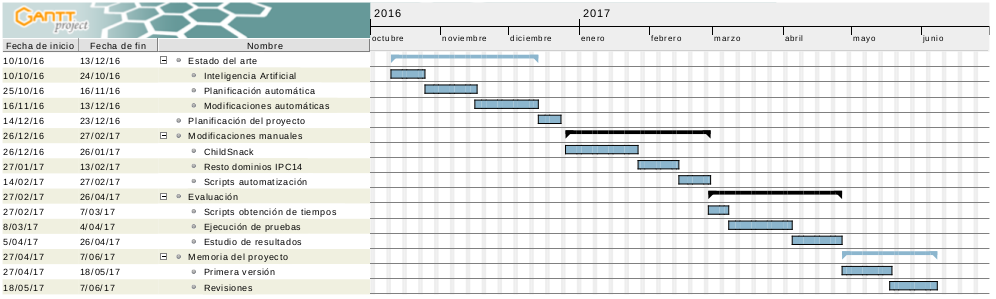
\includegraphics[width=20cm, height=11cm]{diagramaGantt}
        \caption{Diagrama de Gantt del proyecto}
    \end{figure}
    \newpage
    \end{landscape}
    
    \newpage
    
    
    \begin{itemize}
        \item \textbf{Estado del arte}: el primer paso que se ha dado ha sido investigar sobre lo que se ha hecho en el campo de estudio en el que se va a trabajar. En esta fase la mayor parte de la sección de la memoria que lleva este mismo título ha sido redactada mientras que en otra se ha dejado un pequeño esquema minimalista sobre la materia que sirviera simplemente para saber lo que se ha hecho en este campo para tenerlo en cuenta al implementar la solución. Estas partes que no han sido redactadas para poder ser incluidas directamente en este proyecto han sido luego desarrolladas en la fase de redacción de la memoria del proyecto. Como se puede ver el en órden cronológico de las subtareas, se ha seguido un órden que implique pasar de lo más genérico a cada vez lo más concreto en relación con el tema de este trabajo.
        
        \begin{itemize}
            \item \textbf{Inteligencia artificial}: como ya se tenían ciertas nociones sobre este área, la búsqueda ha ido encaminada a la parte histórica de la inteligencia artificial y sus diferentes secciones para así incluirlo en la memoria.
            \item \textbf{Planificación automática}: antes de empezar este proyecto, ya se había trabajado con planificadores automáticos de \textit{PDDL}. Sin embargo, en estos trabajos previos el planificador operaba como una caja negra. Por tanto, esta sección ha sido muy necesaria para así poder interpretar de manera más acertada los resultados obtenidos tras la planificación automática.
            \item \textbf{Modificaciones automáticas}: como se ha reflejado en la memoria, existe trabajo previo de otros investigadores que han realizado programas para automatizar la representación de dominios en \textit{PDDL}, siendo algunos de ellos independientes o dependientes de dominio. El código de las modificaciones independientes de dominio más prometedoras que se han conseguido ejecutar con éxito han sido incluidas en la sección de pruebas de esta memoria.
        \end{itemize}
        
        \item Modificaciones manuales: al estudiar un dominio, es posible encontrar la forma de modificar la representación del mismo para reducir la búsqueda del planificador para así obtener soluciones óptimas y completas en un menor tiempo de búsqueda respecto a la versión original.
        
        \begin{itemize}
            \item \textbf{ChildSnack}: este es el principal dominio con el que se han realizado todas las pruebas y por ello se ha dedicado más tiempo a este dominio que a la suma del tiempo dedicado a todos los demás dominios analizados.
            \item \textbf{Resto dominios \textit{IPC}14}: para intentar generalizar algunas de las conclusiones de este proyecto, se han analizado otros dominios de la misma edición en la que se presentó el dominio \textit{ChildSnack} a la \textit{IPC}. Finalmente se han descartado estos resultados debido a la complejidad de la inclusión de estos resultados con el fin inicial que se tenía de dar una visión más global. Sin embargo, este trabajo al haber sido realizado, se incluye en la planificación real del proyecto.
            \item \textbf{Scripts automatización}: algunas de las modificaciones realizadas a mano en el dominio de \textit{ChildSnack} se han automatizado mediante scripts para así poder transformar de manera automática los problemas del dominio original.
        \end{itemize}
        
        \item \textbf{Evaluación}: en esta fase se han evaluado las distintas versiones de \textit{ChildSnack} con varios planificadores automáticos.
        
        \begin{itemize}
            \item \textbf{Scripts de obtención de tiempos}: se ha creado un script que dado un dominio, una carpeta de problemas y uno de los planificadores para los que está diseñado el dominio, devuelve un archivo de texto plano con todos los tiempos de ejecución, la calidad de la solución así como guarda el plan en caso de haber encontrado la solución al problema.
            \item \textbf{Ejecución de pruebas}: esta fase ha consistido en la ejecución del script con los distintos parámetros de entrada y comprobación de una muestra de los resultados para verificar que no ha habido ningún problema en la ejecución.
            \item \textbf{Estudio de resultados}: una vez se ha verificado que los datos obtenidos son correcto, es necesario interpretarlos ya que la comparación de los mismos determinará su exposición en la memoria.
        \end{itemize}
        
        \item \textbf{Memoria del proyecto}: una vez se han realizado todas las pruebas, se han documentado todo el proceso seguido así como se ha dejado por escrito la interpretación de los resultados obtenidos y las líneas futuras de investigación. Antes de empezar esta fase, únicamente estaba redactada parte de la sección del estado del arte.
        
        
        \begin{itemize}
            \item \textbf{Primera versión}: se ha realizado una primera versión de todo el proyecto para entregar a la tutora y que a partir de esta realizase las anotaciones correspondientes de aquello que era necesario modificar.
            \item \textbf{Revisiones}: las posteriores versiones de la memoria han sido trabajadas tanto a partir de la totalidad de la memoria en distintas revisiones como mediante revisiones concretas de cada una de las secciones de la memoria.
        \end{itemize}
    \end{itemize}
    
    \paragraph{}
    Resumiendo, entre la fecha de inicio y la fecha de finalización del proyecto han trascurrido \\ $341 d\´ias = \ceil{\frac{241 d\´ias}{7 d\´ias/semana}} = 35 semanas$. Si estimamos una media de $13 horas/semana$ a este proyecto, el total de horas dedicadas al proyecto por el alumno es de \textbf{$35 semanas * 13 horas/semana=455 horas$}. Estas horas incluyen las horas invertidas en tutorías especificadas a continuación pero no las horas de ejecución de las pruebas automatizadas.
    
    \paragraph{}
    La planificación ha estado fuertemente influida por las diversas reuniones entre el alumno y la tutora. A continuación se incluye esta información que servirá tanto para plasmar la planificación de este proyecto como para la estimación ulterior de la estimación de gasto en recursos humanos para la realización de este proyecto.
    \begin{enumerate}
        \item 21 de septiembre de 2016.
        \item 10 de octubre de 2016.
        \item 25 de octubre de 2016
        \item 23 de noviembre de 2016
        \item 14 de diciembre de 2016
        \item 20 de febrero de 2017
        \item 14 de marzo de 2017
        \item 4 de abril de 2017
        \item 27 de abril de 2017
        \item 24 de mayo de 2017
        \item 29 de mayo de 2017 
    \end{enumerate}
    
    \paragraph{}
    La duración media de estas reuniones ha sido de en torno a 105 minutos, por lo tanto se estima el número de horas invertidas en estas tutorías en \\ $\ceil{1.75 horas/tutor\´ia * 11 tutor\´ias} = 20 horas$. Se estima a su vez que para 6 de estas tutorías ha sido necesario el trabajo previo de $2 horas$ por parte de la tutora, sumado a $12 horas$ dedicadas para las distintas revisiones de la memoria, lo que hace un total de \\ $20 + 6 * 2 + 12 = 44 horas$. Esta cifra será más adelante utilizada para estimar el coste económico de recursos humanos.
    
    \subsubsection{Estimación de costes económicos}
    
    \paragraph{}
    Esta sección versa sobre el coste económico de la realización de este proyecto en caso de haberse tenido que realizar sin contar con ningún material previo (como pueda ser un ordenador de sobremesa) ni con la idiosincracia de pago de personal académico en la universidad. Es decir, la estimación de costes que se muestra toma como marco de referencia la empresa privada así como la separación de trabajadores según las áreas de trabajo que se pueden encontrar en empresas tecnológicas grandes. Según las recomendaciones de Bruselas acatadas por España en el año 2013, se considera una empresa grande a partir de 250 trabajadores\cite{empresaGrande}.
    
    \setcounter{subsubsubsection}{0}
    \subsubsubsection{Recursos materiales}
    \begin{table}[H]
    \centering
    \caption{Recursos materiales}
    \begin{tabular}{|c|c|c|c|c|c|}
    \hline
    \textbf{Concepto}      & \textbf{Unidades} & \textbf{Coste/u} & \textbf{Total} & \textbf{Amortización/mes} & \textbf{Amortizado(8meses)} \\ \hline
    Ordenador & 1                           & 649\euro                     & 649\euro                  & 2,08\%                                      & 107,99\euro                                       \\ \hline
    Pantalla & 1                           & 79\euro                      & 79\euro                   & 2,08\%                                      & 13,15\euro                                        \\ \hline
    Router                 & 1                           & 22\euro                      & 22\euro                   & 2,08\%                                      & 3,66\euro                                         \\ \hline
    \textbf{Total}         & -                           & -                       & 750\euro                  & -                                           & 124,8\euro                                        \\ \hline
    \end{tabular}
    \end{table}
    
    \paragraph{}
    Antes de poder estimar el coste de materiales fungibles, es necesario calcular las horas de electricidad que han sido necesarias para que el ordenador estuviese encendido con el fin de realizar este proyecto. Para ello hay que añadir a las horas de trabajo del alumno frente al ordenador el número de horas de ejecución de las pruebas.
    
    \paragraph{}
    Teniendo en cuenta que todos los artículos y libros citados en la bibliografía han sido consultados a través del ordenador, las únicas horas del proyecto que no se ha utilizado este dispositivo es cuando el alumno se encontraba en una tutoría del proyecto. Por tanto, el número de horas en las que se ha hecho uso del ordenador sin contar las horas de pruebas es de $455 horas - 20 horas = 435 horas$.
    
    \paragraph{}
    Respecto a las horas necesarias para ejecutar las diversas pruebas, primero hay que tomar en cuenta que aunque en la versión que se ha presentado de este trabajo existan 12 dominios distintos de Childsnack, antes de cribar las versiones menos prometedoras el número de estos dominios era de 16 dominios. Estos 4 dominios descartados eran de baja calidad por lo que para esta estimación se asumirá que únicamente resolvían 2 de los 20 problemas en 30 segundos cada uno, por lo que para simplificar la estimación al ser un tiempo nimio esta cantidad no será tomada en cuenta. Teniendo en cuenta que el tiempo límite de búsqueda de los planificadores es de 30 minutos y que dichas pruebas se ejecutaron 2 veces, el tiempo consumido en la prueba de estos 4 dominios descartados es de $4 * (0.5 horas/problema * 18 problemas)/ejecuci\´on * 2 ejecuciones = 72 horas$. Esta cifra corresponde al número de horas de ejecución necesarias por cada planificador utilizado. Como se han utilizado dos planificadores, el número total será: $72 horas/planificador * 2 planificadores = 144 horas$.
    
    \paragraph{}
    De la versión final se han conservado los tiempos de ejecución para cada planificador, ya que dichos resultados han sido analizados en la sección de evaluación de resultados. Por tanto, teniendo en cuenta que estas pruebas también se han realizado 2 veces, que se han realizado las pruebas con 2 planificadores y tomando la simplificación de descartar el tiempo de las ejecuciones en las que se ha resuelto el problema y añadir un total de $3 horas/ejecuci\´on * 2 ejecuciones = 6 horas$ horas que es un tiempo superior al de la suma del tiempo necesario para la obtención de todas las soluciones para todos los problemas de todas las versiones, obtenemos: \\
    
    $97 problemas no resueltos MFF/iteraci\´on * 2 iteraciones + $ \\
    $42 problemas no resueltos LPG-td/iteraci\´on * 2 iteraciones$ \\
    $= 278 problemas no resueltos * 0.5horas/problema no resuelto = 139 horas$
    
    Por tanto, el número de horas de electricidad necesarias para alimentar el ordenador durante este proyecto será de $435 + 144 + 6 + 139 horas = 724 horas$ de luz necesarias.
    
    \paragraph{}
    El coste de materiales fungibles es el siguiente:
    
    \begin{table}[]
    \centering
    \caption{Coste de materiales fungibles}
    \label{my-label}
    \begin{tabular}{|c|c|c|c|}
    \hline
    \textbf{Concepto}                         & \textbf{Unidades}      & \textbf{Coste/u}          & \textbf{Total}              \\ \hline
    Material para escribir                    & 1                      & 9                         & 9                           \\ \hline
    Hora de electricidad                      & 724                    & 0.1358\euro/KWhora        & 98,32                       \\ \hline
    \multicolumn{1}{|c|}{Conexión a internet} & \multicolumn{1}{c|}{8} & \multicolumn{1}{c|}{19,2} & \multicolumn{1}{c|}{153,6}  \\ \hline
    \multicolumn{1}{|c|}{\textbf{Total}}      & \multicolumn{1}{c|}{-} & \multicolumn{1}{c|}{-}    & \multicolumn{1}{c|}{260,92} \\ \hline
    \end{tabular}
    \end{table}
    
    \paragraph{}
    Por tanto, la estimación de gastos materiales totales para este proyecto es de \\ $124,8€ + 260,92€ = 385,72€$. A esta cantidad habría que añadirle la cantidad no amortizada en los 8 meses de duración de proyecto que sin embargo sin necesarios para comprar el material para desarrollar este proyecto. Es decir, sería necesario disponer a su vez de $750€ - 124,8€  = 625,2€$ de inversión inicial.
    
    \paragraph{}
    Se quiere volver a insistir en que estos datos son estimatorios y simplificados. Otros gastos como el gasto de luz para la iluminación o la calefación durante el invierno han sido descartados.
    
    \subsubsubsection{Recursos humanos}
    \paragraph{}
    Para este proyecto se pueden dividir las tareas realizadas en tantos empleados como la imaginación pueda dar de sí. Estas distintas versiones podrían luego ser estimadas y con ello extraer el coste económico correspondiente a la remuneración de estos trabajadores. Sin embargo, para que esta estimación sea más realista, se va a asumir como coste de desarrollo de este proyecto la composición real que ha tenido (una tutora y un alumno) pero cambiando dichos roles por su equivalente en la empresa privada (como puede ser el project manager y el programador raso).
    
    \begin{table}[H]
    \centering
    \caption{Coste recursos humanos}
    \label{my-label}
    \begin{tabular}{|c|c|c|c|}
    \hline
    \textbf{Posición} & \textbf{Coste/hora} & \textbf{Horas} & \textbf{Total} \\ \hline
    Project manager   & 35                  & 44             & 1.540\euro           \\ \hline
    Programador       & 25                  & 455            & 11.375\euro          \\ \hline
    Total             & -                   & -              & 12.915\euro          \\ \hline
    \end{tabular}
    \end{table}
    
    \subsubsubsection{Coste total}
    
    \paragraph{}
    El coste total de este proyecto será igual al sumatorio de los costes de los materiales fungibles, físicos, el coste en recursos humanos así como el porcentaje de ganancia y el porcentaje de riesgos, como puede ser que el terminal utilizado deje de estar operativo. Este sumatorio se resume en la tabla que se muestra a continuación.
    
    \begin{table}[H]
    \centering
    \caption{Coste total del proyecto}
    \label{my-label}
    \begin{tabular}{|c|c|}
    \hline
    \textbf{Concepto}  & \textbf{Coste} \\ \hline
    Recursos físicos   & 124,8\euro          \\ \hline
    Recursos fungibles & 260,92\euro         \\ \hline
    Recursos humanos   & 12.915\euro         \\ \hline
    Beneficios         & 2.632,14\euro       \\ \hline
    Riesgos            & 1974,11\euro        \\ \hline
    Total              & \textbf{17.906,97\euro}       \\ \hline
    \end{tabular}
    \end{table}
    
    \pagebreak
    
    \subsection{Anexo III: Regulaciones}
    
    \paragraph{}
    En este capítulo se desglosan las regulaciones sociales, legales y económicas de este proyecto.
    
    \subsubsection{Regulaciones sociales}
    \paragraph{}
    Este proyecto está enmarcado dentro del estudio de la planificación automática en \textit{PDDL}. Las conclusiones de este trabajo son útiles principalmente para investigadores de este sector así como también para todo aquel que quiera definir manualmente dominios en \textit{PDDL}, ya que las conclusiones extraídas podrán ser de ayuda para que dicho dominio pueda ser resuelto en el menor tiempo de búsqueda posible.
    
    \subsubsection{Regulaciones legales}
    \paragraph{}
    Para este proyecto la totalidad de herramientas utilizadas han sido de software libre y gratuito. En el caso de los dominios utilizados, haciendo una lectura en diagonal de los artículos de \textit{PDDL} citados se puede ver que la competición \textit{IPC} es una piedra angular en el campo de la investigación de la planificación automática. Para poder testear los dominios presentados a esta competición debido al funcionamiento de \textit{PDDL}, estos necesariamente tienen que ser editables (es decir, la entrada de los problemas no son archivos binarios o de otro tipo que dificulten la edición manual de los mismos). A su vez, la mayoría de los planificadores presentados a esta competición son de software libre y gratuito. Esto permite que se produzca una constante retroalimentación entre investigadores ya que aquellos hallazgos referentes a la planificación son socializados entre los participantes. Esto ha permitido por ejemplo que el planificador de software libre \textit{FF} halla sido presentado por distintos investigadores en distintas versiones del mismo (por ejemplo, \textit{MacroFF} o \textit{Marvin} son implementaciones que parten de \textit{FF}).
    
    \paragraph{}
    Si los planificadores de \textit{PDDL} hubiesen funcionado de otra manera en el que la entrada de los problemas no tuviese que ser necesariamente fácilmente editables y estos dominios no hubiesen sido públicos y accesibles, es muy problable que este proyecto no hubiese existido. Por ello, es imprescindible que tanto esta memoria como los scripts y los dominios utilizados sigan necesariamente esta misma política de compartición de conocimiento para permitir así que otras personas que estén trabajando en la planificación automática puedan sacar el máximo provecho a este trabajo de la misma manera que ha sucedido para la realización de este proyecto. Por tanto, además de encontrar la memoria de este proyecto en formato \textit{PDF} en la biblioteca de la Universidad Carlos III de Madrid, será posible encontrar todo el código utilizado y la memoria en formato \LaTeX en el repositorio personal del alumno\footnote{https://github.com/asdrgil}.
    
    \paragraph{}
    Dicho esto, las licencias de la memoria y del código del proyecto son las siguientes:
    \begin{itemize}
        \item Todos los dominios y scripts creados que pueden encontrarse en el repositorio personal tienen la licencia \textbf{GPLv3}\footnote{https://choosealicense.com/licenses/gpl-3.0/}.
        \item Esta memoria está sujeta a la licencia de \textbf{Creative Commons \\ Reconocimiento-NoComercial-CompartirIgual} 4.0\footnote{http://creativecommons.org/licenses/by-nc-sa/4.0/}.
    \end{itemize}
    
    \subsubsection{Regulaciones económicas}
    \paragraph{}
    Este proyecto puede ayudar a definir mejores dominios en \textit{PDDL}. Sin embargo al no haber desarrollado ningún programa independiente de dominio que realice esta tarea, no es posible obtener rédito económico inmediato de manera directa a partir del trabajo desarrollado.
    
    \pagebreak
    
    \subsection{Anexo IV: Summary of this work}
    
    \paragraph{}
    This section includes an English global summary of the whole project.
    \subsubsection{Abstract}
    \paragraph{}
    This work is a study that tries to shed light on the possibility of reducing the search time and improve the solution's quality by means of variations of the representation of the domains and problems of automated planning. Hence, an empiric study has been made where several modified versions of domains and problems -some of them generated by hand, others generated by domain independent software from other developers- have been used as the input files for planning.
    
    \paragraph{}
    With this work it is expected to prove the relation between the results of planning and the representation of domains and problems, as well as the importance of the election of the planner, as the results of the same representation with different planners vary. In brief, the suitability of certain domain and problem representations could vary depending on the planner used.
    
    \paragraph{}
    The conclusions obtained from this work are that it confirms the initial hypothesis saying that the variation of the representation of the domains and problems could be the reason of substantial variations in both the search times and the quality of the solutions obtained; these results depend on the planner used. There is still a long path to be travelled regarding the domain independent software focused on modifying the representation of problems and domains as the results of the versions obtained from the execution of these programs where exceeded by some of the manual domains.\\ \\ \\
    
    \paragraph{}
    \textbf{Keywords}: \textbf{automated planning (AP)}, \textbf{representatation in AP}, \textbf{PDDL}
    
    \pagebreak
    
    
    \subsubsection{Introduction}
    \paragraph{}
    This is an investigation work that tries to find out the correlation in automated planning between different representation forms of the same problem to be solved and the results obtained after the execution of different planners for the different representations.
    
    \paragraph{}
    Within the next sections it can be found the state of the art of this problem, where it will be explained from the most generic section (artificial intelligence) to the most specific sections regarding the different types of domain independent software aimed to modify the representations of both problems and domains in \textit{PDDL}.
    
    \paragraph{}
    Once it has been explained the state of the art of the investigation of this subject, it will be introduced the domain and problems to be modified. This domain will be modified both by hand and using domain independent software. The different versions of the original domain and problems that will be obtained from these modifications will be then used as input for different planners and the result of the planification made by these planners will be collected.
    
    \paragraph{}
    The results obtained will be then compared an analyzed and some conclusions will be raised based on these results. It is known that due to the fact of the limitation of the number of planners used as well as the fact that only one type of problem is being tested, the generalization of the conclusions raised in this document are limited and could vary among different planners and problems. However, as it can be seen in the following sections, these limitations are taken into account in the conclusions obtained and therefore this could just mean that this work could be enlarged with a greater amount of tryouts of different domains, problems and planners.
    
    \pagebreak
    \setcounter{subsubsubsection}{0}
    \subsubsection{State of the art}
    
    \paragraph{}
    In this section, it will be explained the state of the art of the area where this work is encapsulated. It will be explained from the most generic area (artificial intelligence) to the most concrete, automated planning.
    \setcounter{subsubsubsection}{0}
    \subsubsubsection{Artificial intelligence}
    
    \paragraph{}
    This section includes the definition and some historical milestones of artificial intelligence. \\
    
    \textbf{9.4.3.1.1 Definition of artificial intelligence}
    
    \paragraph{}
    Commonly the Darthmounth conferences of 1956 are considered the germ of artificial intelligence as a research area. These conferences had the objective of studying all the aspects of the intelligence so that it could be described with an accuracy such that a computer could simulate it. The organizer of these conferences, J. McCarthy, coined the term \textit{artificial intelligence} as \textit{"the science and the engineering dedicated to the creation of intelligent machines, specially intelligent computer programs"}.
    
    \paragraph{}
    When the term became popular, several definitions aroused. Stuart J. Russel and Peter Norvig classified them in the following groups:
    \begin{itemize}
        \item Those who defined artificial intelligence as systems that \textbf{could think like humans}.
        \item Those who defined artificial intelligence as systems that \textbf{could act like humans}.
        \item Those who defined artificial intelligence as systems that \textbf{could think rationally}.
        \item Those who defined artificial intelligence as systems that \textbf{could act rationally}.
    \end{itemize} \\
    
    \textbf{9.4.3.1.2 Evolution of artificial intelligence}
    
    \paragraph{}
    Even though the Turing machine was an important preceeding for the development of artificial intelligence, the neural network model of 1943 developed by McCulloch and Pitt it is nowadays considered the first work enclosed in the artificial intelligence field. In this work, they proved that the Turing machine could be implemented using a finite neural network.
    
    The different achievements and phases of artificial intelligence could be summarized as follows:
    
    \begin{itemize}
        \item[\textbf{1957}] General Problem Solver is developed. It was designed to be an universal problem solver. It is the main aforegoing of automated planning.
        \item[\textbf{1959}] Creation of the simple perceptron.
        \item[\textbf{1972}] Creation of the programming language Prolog, which will be later proposed as the native language for the fifth generation machines.
        \item[\textbf{1980-1993}] Fifth generation project: project from the government of Japan aimed to lead the next computer revolution.
        \item[\textbf{1997}] A supercomputer developed by IBM, Deep Blue, wins a six games match against the chess world champion.
    \end{itemize}
    
    \subsubsubsection{Automated planning}
    
    \paragraph{}
    This section contains the basic information about automated planning.
    
    \textbf{9.4.3.2.1 Definition}
    \paragraph{}
    Succintly, automated planning could be defined as \textit{"the art and practise of thinking before acting"}. A more technical definition would be that automated planning is the discipline of artificial intelligence focused on the development of solutions of mathematical models, being theses ones solved by programs that take the description of a particular instance of a model and automatically compute it's solution.
    
    \textbf{9.4.3.2.2 Common elements of planners}
    
    \paragraph{}
    All the planners have these three components:
    \begin{itemize}
        \item \textbf{The conceptual model}, which is the formal definition of the task to be solved as well as the solution's structure.
        \item \textbf{The representation language}, which is the way the problem and the environment are defined.
        \item \textbf{The algorithm}, which is the technique used to solve the problem.
    \end{itemize}
    
    \textbf{9.4.3.2.3 Computational complexity of planning}
    
    \paragraph{}
    In this section, it will be exposed the minimum, maximum and average computational complexity of automated planning.
    
    \paragraph{}
    The minimum computational complexity of automated planning would be a problem with a single operator of size one which it's only effect would be modifying this input predicate (eliminating it or modifying it's value if it's numeric) and an input problem defining a single initial predicate and a single goal predicate. This problem will only have one possible action to do and a single predicate as input choice. All in all, the minimum computational complexity of the most basic input problem possible would be the minimum possible complexity. That is to say, \textbf{O(1)}.
    
    \paragraph{}
    As the possibilities of input problems, domains and their corresponding representations is infinite, it is not possible to define an average computational complexity for automated planning.
    
    \paragraph{}
    The maximum computational complexity for automated planning is the maximum possible complexity for any kind of problem, which is \textbf{NP-hard}.
    
    \textbf{Planners used} \\
    
    \paragraph{}
    The planners used in this project are:
    \begin{itemize}
        \item \textbf{Metric-FF}: is a domain independent planner that allows to operate with \textit{PDDL 2.1} sentences as well as numeric digits sentences. It is an extension from the planner \textit{FF} used to solve linear tasks. For the search process, it uses the \textit{Enforced Hill Climbing (EHC)} algorithm, which is a variation of \textit{Hill Climbing} algorithm based on local search, which in case of failing in the search of better successors (due to local minimums) it uses breadth first search algorithm.
        \item \textbf{Fast Downward}: its a domain independent progressive planner. It's heuristic it's called casual graph heuristic.
        \item \textbf{LPG}: the planner \textit{Local Search Planner (LPG)} it's a planner whose first version was launched in 2003. The core of this planner is based on stochastic local search and the temporal action graphs (\textit{TA_graphs}).
    \end{itemize}
    
    \textbf{9.4.3.2.4 Automatic domain and problems modificators} \\
    \paragraph{}
    In this section it will be explained the automatic modificators used for the tests. A more complete overview of the state of the art of these modificators can be found in the Spanish section of the state of the art included in this memory.
    
    The automatic modificators used in the tests are:
    \begin{itemize}
        \item \textbf{Automatic macrooperators generators}: they join several operators in a single operator in order to function as a shortcut for the planner. These macrooperators tend to be of a greater size than the original operators, which increases the branching factor. The balance of these beneficts and their losts is called the utility problem. The automatic macrooperator used in the tests is called \textit{Planning Task Transformer (PTT)}.
        \item \textbf{Representation of predicates with numeric digits}: in some of the predicates, it does not matter it's identificator, what it really matters for planning is the number of these predicates. If this is the case, these predicates can be substituted by numerical functions.
        \item \textbf{Representation of predicates with numeric predicates}: this representation is based on the same principle of the numeric representation with digits, the difference is that in this case the numeric representation is not with digits but with predicates. This provides the advantage that while not all planners allow numerical digit problems, all of them can process numerical predicates.
    \end{itemize}
    
    \pagebreak
    
    \subsubsection{Work developed}
    \setcounter{subsubsubsection}{0}
    \subsubsubsection{Technologies used}
    \paragraph{}
    It has been used software from third parties that in every phase of the development of this work it has always been free software. The programming languages used for the development of this project are:
    \begin{itemize}
        \item \textbf{Python}: used for some of the scripts.
        \item \textbf{Bash}: used for some the rest of the scripts.
        \item \textbf{PDDL}: used for the domain and problems representation.
    \end{itemize}
    
    \paragraph{}
    Additionally, \LaTeX{} was used for writing this document, Git was used for the control version of both the code and the memory, Sharelatex was used to edit this document and Gedit was the editor used for programming.
    
    \subsubsection{Domains developed}
    All the domains are modifications of the domain and problems presented to the \textit{IPC} 2014 under the name of \textit{Childsnack}. The summary of all the changes made by all the versions that will be tested is the following one:
    \begin{itemize}
        \item \textbf{Original version}: unmodified version of \textit{Childsnack}.
        \item \textbf{Version 01}: it uses macrooperators. It joins the operators \cool{move\_tray} with \cool{serve\_sandwich} and with \cool{serve\_sandwich\_no\_gluten}, it deletes the operator \cool{move\_tray} and includes the operator \cool{move\_tray\_kitchen} so that trays cannot move between tables.
        \item \textbf{Version 02}: it changes the operator \cool{make\_sandwich} so that it cannot accept as input a gluten free component and a gluten free bread in order to avoid labelling sandwich as if they contained gluten when they do not.
        \item \textbf{Version 03}: it uses macrooperators. The only operators that this version has are: \\ \cool{make\_sandwich\_move\_tray\_serve\_sandwich\_no\_gluten\_move\_tray\_kitchen}, \\ \cool{make\_sandwich\_move\_tray\_serve\_sandwich\_move\_tray\_kitchen} and \\ \cool{move\_tray\_kitchen}.
        \item \textbf{Version 05}: manual numeric version with propositions.
        \item \textbf{Version 08}: manual numeric version with digits.
        \item \textbf{Version 09}: it agglutinates several predicates in one. It deletes the predicate \cool{(waiting ?c ?p)} as now the child location it is stored in the predicates \cool{(not\_allergic\_gluten ?c ?p)} and \cool{(allergic\_gluten ?c ?p)}.
        \item \textbf{11 version}: it changes the negative predicates for the negation of the positive ones. The predicates \cool{(not\_allergic\_gluten ?c)} and \cool{(served ?c)} are now expressed as \cool{(not (allegic\_gluten ?c))} and \cool{(not (waiting ?c))} respectively.
        \item \textbf{Version 12}: this version slices the planning process into several phases which cannot be executed until the previous phases are finished.
        \item \textbf{Version PTT}: it is the same version as the original version, as \textit{PTT} was unable to find any macrooperator for this domain.
        \item \textbf{Automated numeric propositions version}: it is generated by \textit{Baggy}.
        \item \textbf{Automated numeric digits version}: it is a numeric digits version generated by a domain independent software whose domain varies slightly from the manual numeric version with digits.
    \end{itemize}
    
    \pagebreak
    
    \subsubsection{Obtained results}
    \paragraph{}
    The tests where made with the planners \textit{Metric-FF}, \textit{LPG-td} and \textit{Fast Downward}. However, the results of the execution of the last planner mentioned are not included in this memory as it did solve less than 10\% of the total number of all problems from all versions. Therefore, this made it almost impossible to interpret the obtained results.
    
    \paragraph{}
    The metrics used to determine the quality of each version are: the number of problems solved for each planner, the time taken for solving these problems and the quality of the plans. The time limit for each problem was 30 minutes, as it is stipulated in the \textit{IPC} competitions.
    
    \paragraph{}
    The results obtained with these metrics were compared separately among the different planners and these results were easily interpreted in the case of \textit{Metric-FF}, but as \textit{LPG-td} was not deeply understood, the explanations of these results are not so clear.
    
    \paragraph{}
    Finally, in order to prove that the results among these two planners are not correlated, the Pearson correlation index was used to compare the average \textit{IPC} time results of each of the version. The value obtained when performing this operation is \textbf{-0.6256}, which means that the versions which are good for one of the planners will outperform with the other one.
    
    \pagebreak
    
    \subsubsection{Conclusions and future work}
    
    \paragraph{}
    In this section, it will be explained the conclusions taken from this project and how this project could be continued.
    
    \setcounter{subsubsubsection}{0}
    \subsubsubsection{Conclusions}
    \paragraph{}
    The conclusions obtained from the development of this work could be summarized as follows:
    \begin{itemize}
        \item Variations of the representation of both problems and domains can make a great difference in the planning performance (understanding this performance as the number of problems solved, time taken and quality of these plans).
        \item There is still a long path to be traveled in the creation of software that automatically changes the representation of both domains and problems, as the results of the automatically modified versions where worse than some of the versions made by hand.
        \item The suitability of the different representations varies depending on the type of planner used.
    \end{itemize}
    
    \subsubsubsection{Future work}
    The future work to be done in this area would be to make the same type of tests but with more domains and more planners. Then, the long term future work goal would be to program software capable of finding the best representation for each planner.
    
    \pagebreak
    
    \bibliographystyle{unsrt}
    \addcontentsline{toc}{section}{Bibliografía}
    \bibliography{sample}
    
    \end{document}